% !TEX program = xelatex
\documentclass[UTF8,fontset=fandol,a4paper,11pt]{ctexart}
\usepackage[margin=21mm,top=23mm,bottom=22mm,headheight=16pt]{geometry}
\usepackage{amsmath,amssymb,mathtools,bm}
\usepackage{tikz}
\usetikzlibrary{arrows.meta,calc,angles,quotes,patterns}
\usepackage{xcolor,booktabs,array,longtable,enumitem,fancyhdr,needspace}
\usepackage[unicode,hidelinks]{hyperref}
\definecolor{ink}{HTML}{24343C}
\definecolor{accent}{HTML}{166A70}
\definecolor{muted}{HTML}{65747A}
\definecolor{rulegray}{HTML}{D4DDE0}
\definecolor{warm}{HTML}{966037}
\color{ink}
\setlength{\parindent}{2em}
\setlength{\parskip}{4pt}
\linespread{1.12}
\AtBeginDocument{\setlength{\abovedisplayskip}{6pt plus 2pt minus 1pt}
\setlength{\belowdisplayskip}{6pt plus 2pt minus 1pt}
\setlength{\abovedisplayshortskip}{0pt plus 1pt}
\setlength{\belowdisplayshortskip}{4pt plus 1pt}}
\setlist[enumerate]{label=(\arabic*),leftmargin=2.3em,itemsep=3pt,topsep=4pt}
\setlist[itemize]{leftmargin=2em,itemsep=2pt,topsep=4pt}
\allowdisplaybreaks[1]
\setlength{\emergencystretch}{2em}
\setcounter{secnumdepth}{0}
\providecommand{\tightlist}{\setlength{\itemsep}{0pt}\setlength{\parskip}{0pt}}
\ctexset{section={format=\Large\bfseries\color{accent},beforeskip=10pt,afterskip=9pt},
subsection={format=\normalsize\bfseries\color{accent},beforeskip=10pt,afterskip=4pt},
subsubsection={format=\normalsize\bfseries,beforeskip=8pt,afterskip=3pt}}
\pagestyle{fancy}
\fancyhf{}
\fancyhead[L]{\small\color{muted}物理学难题集萃}
% 页眉仅保留书名；版本名称只在封面显示。
\fancyfoot[L]{\small\color{muted}\chapterlabel}
\fancyfoot[R]{\small\thepage}
\renewcommand{\headrulewidth}{0.4pt}
\renewcommand{\footrulewidth}{0pt}
\newcommand{\dd}{\mathop{}\!\mathrm{d}}
\newcommand{\vect}[1]{\bm{#1}}
\newcommand{\tagline}[1]{\noindent{\small\color{muted}#1}\par}
\newcommand{\result}[1]{\begin{equation*}\boxed{#1}\end{equation*}}
\newcommand{\figcaption}[1]{\par\vspace{2pt}{\small\color{muted}#1}\par}
\newcommand{\teach}[2]{\Needspace{4\baselineskip}\subsection*{讲解要点与追问}#1\par\smallskip\noindent\textbf{追问：}#2\par}
\newcommand{\workarea}{\par\vspace{7mm}\noindent{\small\color{muted}作答区}\par\vspace{4mm}
\noindent\textcolor{rulegray}{\rule{\linewidth}{0.3pt}}\par\vspace{16mm}
\noindent\textcolor{rulegray}{\rule{\linewidth}{0.3pt}}\par\vspace{16mm}
\noindent\textcolor{rulegray}{\rule{\linewidth}{0.3pt}}\par\vspace{16mm}
\noindent\textcolor{rulegray}{\rule{\linewidth}{0.3pt}}}
\tikzset{axis/.style={-{Stealth[length=2mm]},thin,color=muted},
motion/.style={-{Stealth[length=2.3mm]},thick,color=accent},
force/.style={-{Stealth[length=2.3mm]},thick,color=warm},
traj/.style={thick,color=accent},guide/.style={dashed,thin,color=muted},
object/.style={thick,color=ink},every node/.style={font=\small}}\widowpenalty=10000\clubpenalty=10000\displaywidowpenalty=10000\newcommand{\chapterlabel}{电磁学试题（三）}







\hypersetup{pdftitle={电磁学试题（三）·教师版},pdfauthor={}}

\begin{document}\pdfbookmark[0]{电磁学试题（三）}{cover}

\thispagestyle{empty}\vspace*{22mm}

\noindent{\Huge\bfseries 物理学难题集萃}\par\vspace{12mm}

\noindent{\LARGE 电磁学试题（三）}\par\vspace{12mm}

\noindent{\Large\color{accent}教师版}\par\vspace{9mm}

\noindent\textcolor{accent}{\rule{\linewidth}{1pt}}\par\vspace{9mm}

\noindent 第1--5题\par\vfill\clearpage

\pdfbookmark[1]{题目目录}{contents}\section*{题目目录}

\begin{longtable}{@{}r p{113mm} r@{}}\toprule 题号 & 题目 & 页码\\\midrule

\hyperref[q:1]{1} & \hyperref[q:1]{二维电导与折叠导电曲面的电阻} & \pageref{q:1} \\

\hyperref[q:2]{2} & \hyperref[q:2]{双环网络与无限内接正方形网络} & \pageref{q:2} \\

\hyperref[q:3]{3} & \hyperref[q:3]{双频理想电源驱动的稳态电流} & \pageref{q:3} \\

\hyperref[q:4]{4} & \hyperref[q:4]{三棱柱交流网络与最小补偿电容} & \pageref{q:4} \\

\hyperref[q:5]{5} & \hyperref[q:5]{锯齿电源驱动的RC逐周期暂态} & \pageref{q:5} \\

\bottomrule\end{longtable}

\clearpage

\pdfbookmark[2]{第 1 题 二维电导与折叠导电曲面的电阻}{q1}

\section*{第 1 题\quad 二维电导与折叠导电曲面的电阻}\label{q:1}


在二维金属曲面上，电子数面密度为$n^*$，电子质量$m$、电荷$-e$，热运动平均速率为$\bar v^*$，平均自由程为$\lambda^*$。采用等时自由飞行模型：每段自由飞行时间均为$\tau^*=\lambda^*/\bar v^*$，碰撞清除平均漂移速度，电场在每段飞行中产生附加漂移；忽略磁场。
\begin{enumerate}
\item 定义曲面电流密度$\boldsymbol j^*$为单位横向线长通过的电流，推导$\boldsymbol j^*=\sigma^*\boldsymbol E$及$\sigma^*$。说明系数为何依赖碰撞模型。
\item 一均匀导电薄片由上下两个内半径$R_1$、外半径$R_2$的圆环面和连接其外圆周的高$H$圆柱面组成，$0<R_1<R_2$。片电阻率$\rho^*=1/\sigma^*$恒定，电流从上端内圆周均匀流入，从下端内圆周均匀流出。求两内圆周间电阻。
\end{enumerate}
薄片只沿自身曲面导电，内部空间不导电；两圆环面不经内圆柱面相连。


\begin{center}\begin{minipage}{.98\linewidth}\centering
\begin{tikzpicture}[scale=.75,transform shape]

\fill[muted!8] (-2,0)--(-2,3) arc[start angle=180,end angle=0,x radius=2,y radius=.55]--(2,0) arc[start angle=0,end angle=-180,x radius=2,y radius=.55];
\draw[object] (0,3) ellipse (2 and .55);
\draw[object] (0,3) ellipse (.8 and .22);
\draw[object] (-2,0)--(-2,3);\draw[object] (2,0)--(2,3);
\draw[object] (0,0) ellipse (2 and .55);
\draw[guide] (0,0) ellipse (.8 and .22);
\draw[motion] (.85,3)--(1.8,3) node[midway,above] {$I$};
\draw[motion] (2,2.6)--(2,1);
\draw[motion] (1.8,0)--(.85,0);
\draw[guide] (0,3)--(-2,3) node[midway,above] {$R_2$};
\draw[guide] (0,3)--(.56,3.156) node[midway,above left] {$R_1$};
\draw[axis,<->] (2.7,0)--(2.7,3) node[midway,right] {$H$};
\node[align=center] at (-4.2,1.5) {导电薄片\\内部不导电};

\end{tikzpicture}
\figcaption{图电试3.1\quad 电流经上环面、外柱面、下环面串联，内孔无连接柱面。}
\end{minipage}\end{center}

\Needspace{8\baselineskip}

\pdfbookmark[3]{题型定位}{q1-h0}

\subsection*{题型定位}

先从电子漂移的时间平均定义二维电流密度与片电导，再从曲面电流的横向截线求几何电阻。等时碰撞模型确定微观系数，轴对称电流守恒确定宏观分布。两层计算分别说明平均方式与路径几何，最后把上环面、外柱面、下环面依次串联。

\Needspace{8\baselineskip}

\pdfbookmark[3]{知识点}{q1-h1}

\subsection*{知识点}

电场在碰撞间隔内使电子附加漂移，等时飞行的平均年龄为飞行时长的一半。二维电流密度是每单位横向线长的电流，单位为A/m，片电导与片电阻的单位分别为S与欧姆。局部欧姆定律给$E=\rho^*j^*$，曲面流管在横向宽度$w$处有$j^*=I/w$。轴对称同心圆为等势线，圆环部分宽度随半径改变，柱面部分宽度恒定。

\Needspace{8\baselineskip}

\pdfbookmark[3]{物理图像}{q1-h2}

\subsection*{物理图像}

题图显示内孔与外柱面连接，电流从上方内圈向外走、沿外壁向下、再从下方外圈走回内圈。解图电试3.1A用飞行年龄下的漂移速度三角形表示平均值。图B把三个连续导电区展开，图C沿同一条展开路径画累计电势降，三段的斜率分别随$1/r$变化、保持常量、再随$1/r$增加。

\Needspace{8\baselineskip}

\pdfbookmark[3]{解题入口}{q1-h3}

\subsection*{解题入口}

先用一条横向线段与漂移速度构成的扫过面积计算电子数，再按负电荷方向定义电流。漂移速度先对等时年龄区间积分，再用泊松碰撞的年龄分布计算另一组平均值。几何部分先找同心等势线和对应横向线长，再按电流方向对局部电场积分；上下两环面的径向方向相反，沿电流的电势降低均为正。

\Needspace{8\baselineskip}

\pdfbookmark[3]{标准解法}{q1-h4}

\subsection*{标准解法}


图电试3.1中电流沿上环面向外，再沿外柱面向下，最后沿下环面向内。先求局部电导，再把这三段曲面依次串联。

第（1）问中，电子的平均附加加速度为$\boldsymbol a_d=-e\boldsymbol E/m$。在一次自由飞行开始后的时刻$s$，
\[
\boldsymbol u_d(s)=-\frac e m\boldsymbol E\,s,
\qquad 0\le s<\tau^*.
\]
\begin{center}\begin{minipage}{.98\linewidth}\centering
\begin{tikzpicture}[scale=.85,transform shape]

\draw[axis] (0,0)--(5.1,0) node[right] {$s/\tau^*$};
\draw[axis] (0,0)--(0,3) node[above] {$|u_d|$};
\draw[traj] (0,0)--(2,2.4)--(2,0)--(4,2.4);
\draw[guide] (0,1.2)--(4.3,1.2);
\node[right] at (4.3,1.2) {$eE\tau^*/(2m)$};
\node[below] at (2,0) {$1$};\node[below] at (4,0) {$2$};
\node[left] at (0,2.4) {$eE\tau^*/m$};
\node at (2.5,4.2) {等时碰撞：三角形面积给平均漂移};

\end{tikzpicture}
\figcaption{解图电试3.1A\quad 单次飞行末漂移为平均值的两倍，取平均需要指定碰撞模型。}
\end{minipage}\end{center}
解图电试3.1A中的漂移速度随飞行年龄线性增长，碰撞时清零。等时飞行模型中，稳态观察各电子时，飞行年龄在$[0,\tau^*]$均匀分布，平均飞行年龄为$\tau^*/2$，故
\[
\overline{\boldsymbol u}_d
=\frac1{\tau^*}\int_0^{\tau^*}\boldsymbol u_d(s)\,ds
=-\frac{e\tau^*}{2m}\boldsymbol E.
\]
曲面上取一条与漂移垂直、长$w$的线段，时间$dt$内因定向漂移而净通过它的电子数为
$n^*w|\overline{\boldsymbol u}_d|dt$。计入电子负电荷，约定电流与电子漂移反向，有
\[
\boldsymbol j^*=-n^*e\overline{\boldsymbol u}_d
=\sigma^*\boldsymbol E,\qquad
\boxed{\sigma^*=\frac{n^*e^2\tau^*}{2m}
=\frac{n^*e^2\lambda^*}{2m\bar v^*}}.
\]
$j^*$单位为$\mathrm{A/m}$，因此$\sigma^*$单位为$\mathrm S$，$\rho^*$单位为$\Omega$。二维性改变了数密度、电流密度及其单位；上式的$1/2$来自所设等时飞行的年龄平均，二维性则体现在面密度、片电流密度及对应单位中。

一般年龄平均也可从完整飞行段直接求得。一段时长$T_f$内，年龄从0线性增加到$T_f$，年龄对时间的积分为$\int_0^{T_f}s\mathrm ds=T_f^2/2$。观察许多完整飞行段，平均年龄就是各段年龄积分之和除以总时长，即$[\sum T_f^2/2]/[\sum T_f]$。在稳态长时间极限中，均匀观察时刻得到的年龄平均趋向下式的矩之比。

若改用泊松碰撞模型，平均碰撞间隔为$\tau^*$，稳态平均飞行年龄也是$\tau^*$，电导应为$n^*e^2\tau^*/m$。更一般地，若相邻碰撞间隔为随机量$T_f$，
\[
\langle s\rangle_{\rm age}
=\frac{\langle T_f^2\rangle}{2\langle T_f\rangle},
\qquad
\sigma^*=\frac{n^*e^2}{m}
\frac{\langle T_f^2\rangle}{2\langle T_f\rangle}.
\]
平均自由程与平均速率确定平均碰撞间隔，间隔的二阶矩进一步确定稳态年龄平均。本题等时模型的时长固定，二阶矩为$\tau^{*2}$。

这里的热运动是各向随机的，电场造成的附加漂移则具有确定的平均方向。弱电场近似保持题设的碰撞统计与热运动速率，电子的漂移平均可叠加在热运动上；电子带负电，所以漂移方向与约定电流方向相反。片电流的定义按横向线长计数，对线段宽度$w$求电流有$I=j^*w$，与三维电流按截面积计数使用不同单位。

第（2）问依据轴对称性，每个同心圆周上电势相同，流经任一截线的总电流均为$I$。
\begin{center}\begin{minipage}{.98\linewidth}\centering
\begin{tikzpicture}[scale=.75,transform shape]

\draw[object] (0,0)--(1,0);\draw[object] (1,-.25) rectangle (3,.25);
\draw[object] (3,0)--(4,0);\draw[object] (4,-.25) rectangle (6,.25);
\draw[object] (6,0)--(7,0);\draw[object] (7,-.25) rectangle (9,.25);
\draw[object] (9,0)--(10,0);
\draw[motion] (-.1,.7)--(1,.7) node[midway,above] {$I$};
\node at (2,.85) {上环面};\node at (5,.85) {外柱面};\node at (8,.85) {下环面};
\node[align=center] at (2,-.9) {$w=2\pi r$\\$R_1\to R_2$};
\node[align=center] at (5,-.9) {$w=2\pi R_2$\\高$H$};
\node[align=center] at (8,-.9) {$w=2\pi r$\\$R_2\to R_1$};
\node at (5,-2) {$dR=\rho^*\,ds/w(s)$};

\end{tikzpicture}
\figcaption{解图电试3.1B\quad 三段曲面的电学串联等效，同一电流依次通过各截线。}
\end{minipage}\end{center}
解图电试3.1B将三个导电区按电流方向展开。上端圆环面在半径$r$处的横向线长为$2\pi r$，
\[
j_r^*=\frac I{2\pi r},\qquad
E_r=\rho^*j_r^*=\frac{\rho^*I}{2\pi r}.
\]
从内圆至外圆的电势降低为
\[
\Delta U_1=\int_{R_1}^{R_2}E_r\,dr
=\frac{\rho^*I}{2\pi}\ln\frac{R_2}{R_1}.
\]
外柱面的横向线长恒为$2\pi R_2$，电流沿高方向向下，
\[
j_h^*=\frac I{2\pi R_2},\qquad
\Delta U_2=\frac{\rho^*IH}{2\pi R_2}.
\]
柱面上的每个水平截线都有相同周长，轴向电流密度与电场因而都保持常量。上环面的电流则在越来越长的同心圆上分散，电场随$r$的倒数减小，径向积分自然给出对数。下端圆环面电流沿径向向内，按电流路径积分时$E_r$和$dr$均为负，电势降低仍为正：
\[
\Delta U_3=\frac{\rho^*I}{2\pi}\ln\frac{R_2}{R_1}.
\]
三段依次串联，得到
\[
\boxed{R_{\rm eq}=\frac{\Delta U_1+\Delta U_2+\Delta U_3}{I}
=\frac{\rho^*}{\pi}
\left(\ln\frac{R_2}{R_1}+\frac H{2R_2}\right)}.
\]
\begin{center}\begin{minipage}{.98\linewidth}\centering
\begin{tikzpicture}[scale=.8,transform shape]
\draw[axis] (0,0)--(10.7,0) node[right] {展开路径$s$};
\draw[axis] (0,0)--(0,3.2) node[above] {累计电势降$/\Delta U$};\foreach \y/\lab in {0/0,1.4/0.5,2.8/1}{\draw[thin] (0,\y)--(-.08,\y) node[left] {$\lab$};}
\node[above] at (5,3.5) {$R_1=1,R_2=2,H=2$的三段连续电势降};
\draw[traj] plot coordinates {(0.000000000,0.000000000) (0.062500000,0.028973507) (0.125000000,0.057248788) (0.187500000,0.084858706) (0.250000000,0.111833857) (0.312500000,0.138202774) (0.375000000,0.163992106) (0.437500000,0.189226786) (0.500000000,0.213930170) (0.562500000,0.238124170) (0.625000000,0.261829368) (0.687500000,0.285065125) (0.750000000,0.307849674) (0.812500000,0.330200205) (0.875000000,0.352132944) (0.937500000,0.373663225) (1.000000000,0.394805552) (1.062500000,0.415573659) (1.125000000,0.435980563) (1.187500000,0.456038613) (1.250000000,0.475759538) (1.312500000,0.495154482) (1.375000000,0.514234047) (1.437500000,0.533008326) (1.500000000,0.551486934) (1.562500000,0.569679041) (1.625000000,0.587593395) (1.687500000,0.605238350) (1.750000000,0.622621889) (1.812500000,0.639751644) (1.875000000,0.656634920) (1.937500000,0.673278708) (2.000000000,0.689689708) (2.062500000,0.705874343) (2.125000000,0.721838771) (2.187500000,0.737588906) (2.250000000,0.753130423) (2.312500000,0.768468777) (2.375000000,0.783609212) (2.437500000,0.798556769) (2.500000000,0.813316302) (2.562500000,0.827983395) (2.625000000,0.842650487) (2.687500000,0.857317579) (2.750000000,0.871984672) (2.812500000,0.886651764) (2.875000000,0.901318857) (2.937500000,0.915985949) (3.000000000,0.930653042) (3.062500000,0.945320134) (3.125000000,0.959987227) (3.187500000,0.974654319) (3.250000000,0.989321411) (3.312500000,1.003988504) (3.375000000,1.018655596) (3.437500000,1.033322689) (3.500000000,1.047989781) (3.562500000,1.062656874) (3.625000000,1.077323966) (3.687500000,1.091991059) (3.750000000,1.106658151) (3.812500000,1.121325244) (3.875000000,1.135992336) (3.937500000,1.150659428) (4.000000000,1.165326521) (4.062500000,1.179993613) (4.125000000,1.194660706) (4.187500000,1.209327798) (4.250000000,1.223994891) (4.312500000,1.238661983) (4.375000000,1.253329076) (4.437500000,1.267996168) (4.500000000,1.282663260) (4.562500000,1.297330353) (4.625000000,1.311997445) (4.687500000,1.326664538) (4.750000000,1.341331630) (4.812500000,1.355998723) (4.875000000,1.370665815) (4.937500000,1.385332908) (5.000000000,1.400000000) (5.062500000,1.414667092) (5.125000000,1.429334185) (5.187500000,1.444001277) (5.250000000,1.458668370) (5.312500000,1.473335462) (5.375000000,1.488002555) (5.437500000,1.502669647) (5.500000000,1.517336740) (5.562500000,1.532003832) (5.625000000,1.546670924) (5.687500000,1.561338017) (5.750000000,1.576005109) (5.812500000,1.590672202) (5.875000000,1.605339294) (5.937500000,1.620006387) (6.000000000,1.634673479) (6.062500000,1.649340572) (6.125000000,1.664007664) (6.187500000,1.678674756) (6.250000000,1.693341849) (6.312500000,1.708008941) (6.375000000,1.722676034) (6.437500000,1.737343126) (6.500000000,1.752010219) (6.562500000,1.766677311) (6.625000000,1.781344404) (6.687500000,1.796011496) (6.750000000,1.810678589) (6.812500000,1.825345681) (6.875000000,1.840012773) (6.937500000,1.854679866) (7.000000000,1.869346958) (7.062500000,1.884014051) (7.125000000,1.898681143) (7.187500000,1.913348236) (7.250000000,1.928015328) (7.312500000,1.942682421) (7.375000000,1.957349513) (7.437500000,1.972016605) (7.500000000,1.986683698) (7.562500000,2.001443231) (7.625000000,2.016390788) (7.687500000,2.031531223) (7.750000000,2.046869577) (7.812500000,2.062411094) (7.875000000,2.078161229) (7.937500000,2.094125657) (8.000000000,2.110310292) (8.062500000,2.126721292) (8.125000000,2.143365080) (8.187500000,2.160248356) (8.250000000,2.177378111) (8.312500000,2.194761650) (8.375000000,2.212406605) (8.437500000,2.230320959) (8.500000000,2.248513066) (8.562500000,2.266991674) (8.625000000,2.285765953) (8.687500000,2.304845518) (8.750000000,2.324240462) (8.812500000,2.343961387) (8.875000000,2.364019437) (8.937500000,2.384426341) (9.000000000,2.405194448) (9.062500000,2.426336775) (9.125000000,2.447867056) (9.187500000,2.469799795) (9.250000000,2.492150326) (9.312500000,2.514934875) (9.375000000,2.538170632) (9.437500000,2.561875830) (9.500000000,2.586069830) (9.562500000,2.610773214) (9.625000000,2.636007894) (9.687500000,2.661797226) (9.750000000,2.688166143) (9.812500000,2.715141294) (9.875000000,2.742751212) (9.937500000,2.771026493) (10.000000000,2.800000000)};
\node[below] at (0,-.12) {上内圈};
\node[below] at (2.5,-.12) {上外圈};
\node[below] at (7.5,-.12) {下外圈};
\node[below] at (10,-.12) {下内圈};
\end{tikzpicture}
\figcaption{解图电试3.1C\quad $R_1=1,R_2=2,H=2$的三段连续电势降}
\end{minipage}\end{center}
图C沿上内圈、上外圈、下外圈、下内圈的次序累计电势降低。曲线全程增加，两个转折位置分别对应导电方向从径向变为柱面方向、再变回径向；连接外缘处电势连续，各区域的局部场由各自横向宽度确定。以图中的$R_1=1,R_2=2,H=2$为例，上下环面各贡献$\rho^*I\ln2/(2\pi)$，外柱面贡献$\rho^*I/(2\pi)$，相加正是整条曲线的末端值。

也可用局部矩形薄片电阻$dR=\rho^*\,ds/w(s)$，对两圆环与柱面分别积分，得到同式。这里沿薄片电流路径使用长度与横向宽度，内部空间保持不导电，各段片电阻依次相加。
局部条带长$\mathrm ds$、横向宽$w$，电势降低$\mathrm dU=E\mathrm ds=\rho^*I\mathrm ds/w$，所以$\mathrm dR=\rho^*\mathrm ds/w$。圆环取$\mathrm ds=|\mathrm dr|$、$w=2\pi r$，柱面取$\mathrm ds=\mathrm dh$、$w=2\pi R_2$，三段都具有相同的串联电流。这也说明二维电阻的几何部分取决于长度比，而非内部空腔的横截面积。



\Needspace{8\baselineskip}

\pdfbookmark[3]{关键洞察}{q1-h5}

\subsection*{关键洞察}

微观电导系数随碰撞统计改变，实测片电阻率给定后，几何电阻仍由曲面路径决定。上下环面和外柱面是同一电流先后通过的三个区域，串联的拓扑由外缘连接确定。片电阻以欧姆为单位，局部电阻只取路径长度与横向宽度的比值，不再引入三维导体截面积。

\Needspace{8\baselineskip}

\pdfbookmark[3]{易错点}{q1-h6}

\subsection*{易错点}

平均漂移对稳态年龄分布取平均，等时与泊松碰撞分别给$\tau^*/2$与$\tau^*$。面密度、片电流密度、片电阻率按各自单位使用。圆环横向宽度为$2\pi r$，沿半径变化；下环面沿电流方向积分时电场和路径同时转向。内孔两端之间保持题设的非导电空间，电流只经外缘连接的薄片返回。

\Needspace{8\baselineskip}

\pdfbookmark[3]{课堂讲解建议}{q1-h7}

\subsection*{课堂讲解建议}

先画等时飞行的漂移三角形，比较末速度与时间平均速度，再用随机飞行时长说明按观察时刻统计时，较长飞行段占用的时间也较长。由每次飞行年龄积分的面积$T_f^2/2$与总飞行时长的比值，推得一般平均年龄公式。

宏观部分让学生用一条连续箭头走完整个导电路径，逐段画等势线并写横向宽度。图C用累计电势降把三段串联直接展示出来。最后取零柱高、窄圆环和均匀厚度变化的极限，说明各电阻项分别对应哪一片导电区域。

\Needspace{8\baselineskip}

\pdfbookmark[3]{变式训练}{q1-h8}

\subsection*{变式训练}

\begin{enumerate}
\Needspace{20\baselineskip}
\item 改用泊松碰撞模型，碰撞间隔均值为$\tau^*$，求片电导。
\textbf{解：}变图电试3.1V1的稳态年龄密度为$e^{-s/\tau^*}/\tau^*$，平均年龄$\int_0^\infty s e^{-s/\tau^*}\mathrm ds/\tau^*=\tau^*$。因此平均漂移为$-e\tau^*\boldsymbol E/m$，片电导$\sigma^*=n^*e^2\tau^*/m$。碰撞时长的二阶矩为$2\tau^{*2}$，代入一般年龄公式也得到同样结果。等时模型与泊松模型的平均碰撞间隔相同，年龄分布不同，使电导相差2倍。
\begin{center}\begin{minipage}{.98\linewidth}\centering
\begin{tikzpicture}[scale=.8,transform shape]
\draw[axis] (0,0)--(10.7,0) node[right] {$s/\tau^*$};
\draw[axis] (0,0)--(0,3.2) node[above] {$\tau^*p_{\rm age}$};\foreach \y/\lab in {0/0,1.4/0.5,2.8/1}{\draw[thin] (0,\y)--(-.08,\y) node[left] {$\lab$};}
\node[above] at (5,3.5) {泊松碰撞的稳态年龄分布};
\draw[traj] plot coordinates {(0.000000000,2.800000000) (0.083333333,2.708205081) (0.166666667,2.619419558) (0.250000000,2.533544771) (0.333333333,2.450485293) (0.416666667,2.370148830) (0.500000000,2.292446109) (0.583333333,2.217290786) (0.666666667,2.144599347) (0.750000000,2.074291018) (0.833333333,2.006287670) (0.916666667,1.940513736) (1.000000000,1.876896129) (1.083333333,1.815364155) (1.166666667,1.755849439) (1.250000000,1.698285847) (1.333333333,1.642609415) (1.416666667,1.588758273) (1.500000000,1.536672581) (1.583333333,1.486294462) (1.666666667,1.437567933) (1.750000000,1.390438851) (1.833333333,1.344854843) (1.916666667,1.300765257) (2.000000000,1.258121100) (2.083333333,1.216874984) (2.166666667,1.176981077) (2.250000000,1.138395047) (2.333333333,1.101074018) (2.416666667,1.064976518) (2.500000000,1.030062435) (2.583333333,0.996292972) (2.666666667,0.963630603) (2.750000000,0.932039034) (2.833333333,0.901483160) (2.916666667,0.871929027) (3.000000000,0.843343793) (3.083333333,0.815695695) (3.166666667,0.788954009) (3.250000000,0.763089020) (3.333333333,0.738071987) (3.416666667,0.713875109) (3.500000000,0.690471499) (3.583333333,0.667835151) (3.666666667,0.645940910) (3.750000000,0.624764448) (3.833333333,0.604282234) (3.916666667,0.584471505) (4.000000000,0.565310250) (4.083333333,0.546777176) (4.166666667,0.528851688) (4.250000000,0.511513867) (4.333333333,0.494744448) (4.416666667,0.478524796) (4.500000000,0.462836887) (4.583333333,0.447663289) (4.666666667,0.432987141) (4.750000000,0.418792134) (4.833333333,0.405062495) (4.916666667,0.391782966) (5.000000000,0.378938793) (5.083333333,0.366515702) (5.166666667,0.354499888) (5.250000000,0.342877999) (5.333333333,0.331637121) (5.416666667,0.320764763) (5.500000000,0.310248843) (5.583333333,0.300077677) (5.666666667,0.290239960) (5.750000000,0.280724762) (5.833333333,0.271521510) (5.916666667,0.262619976) (6.000000000,0.254010269) (6.083333333,0.245682822) (6.166666667,0.237628381) (6.250000000,0.229837996) (6.333333333,0.222303010) (6.416666667,0.215015051) (6.500000000,0.207966019) (6.583333333,0.201148082) (6.666666667,0.194553663) (6.750000000,0.188175436) (6.833333333,0.182006311) (6.916666667,0.176039434) (7.000000000,0.170268175) (7.083333333,0.164686121) (7.166666667,0.159287067) (7.250000000,0.154065016) (7.333333333,0.149014164) (7.416666667,0.144128899) (7.500000000,0.139403791) (7.583333333,0.134833592) (7.666666667,0.130413221) (7.750000000,0.126137767) (7.833333333,0.122002479) (7.916666667,0.118002762) (8.000000000,0.114134171) (8.083333333,0.110392408) (8.166666667,0.106773314) (8.250000000,0.103272869) (8.333333333,0.099887181) (8.416666667,0.096612490) (8.500000000,0.093445156) (8.583333333,0.090381659) (8.666666667,0.087418596) (8.750000000,0.084552674) (8.833333333,0.081780707) (8.916666667,0.079099617) (9.000000000,0.076506423) (9.083333333,0.073998244) (9.166666667,0.071572293) (9.250000000,0.069225874) (9.333333333,0.066956380) (9.416666667,0.064761289) (9.500000000,0.062638161) (9.583333333,0.060584638) (9.666666667,0.058598437) (9.750000000,0.056677352) (9.833333333,0.054819247) (9.916666667,0.053022059) (10.000000000,0.051283789)};
\node[below] at (0,-.12) {$0$};
\node[below] at (5,-.12) {$2$};
\node[below] at (10,-.12) {$4$};
\end{tikzpicture}
\figcaption{变图电试3.1V1\quad 泊松碰撞的稳态年龄分布}
\end{minipage}\end{center}

\Needspace{20\baselineskip}
\item 薄片由厚度$d$、三维电导率$\sigma$的均匀材料制成，求二维与三维电阻率的关系。
\textbf{解：}变图电试3.1V2取横向长度$w$的截线，对应实体截面积为$dw$。电流$I=j\,dw=j^*w$，所以$j^*=dj=\sigma dE$，片电导为$\sigma^*=\sigma d$，片电阻率为$\rho^*=\rho/d$。将其代入折叠曲面的几何结果，$R=\rho[\ln(R_2/R_1)+H/(2R_2)]/(\pi d)$。材料和曲面形状固定时，厚度加倍使每条通道的导电能力加倍，电阻减半。
\begin{center}\begin{minipage}{.98\linewidth}\centering
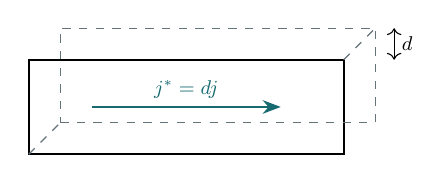
\begin{tikzpicture}[scale=.8,transform shape]
\draw[thick] (0,0) rectangle (5,1.5);\draw[guide] (.5,.5)--(5.5,.5)--(5.5,2)--(.5,2)--cycle;\draw[guide] (0,0)--(.5,.5);\draw[guide] (5,1.5)--(5.5,2);\draw[<->] (5.8,1.5)--(5.8,2) node[midway,right] {$d$};\draw[motion] (1,.75)--(4,.75) node[midway,above] {$j^*=dj$};
\end{tikzpicture}
\figcaption{变图电试3.1V2\quad 片电流是厚度方向积分后的实体电流密度}
\end{minipage}\end{center}

\Needspace{20\baselineskip}
\item 分别取柱高趋零与圆环变窄的几何极限，写出各剩余电阻。
\textbf{解：}变图电试3.1V3中上下两面仍只在外缘连接，$H\to0$使柱面项趋零，留下两个圆环串联的$R=(\rho^*/\pi)\ln(R_2/R_1)$。若保持$H>0$而令$R_1\to R_2$，两个环面径向路径同时缩短，留下外柱面$R=\rho^*H/(2\pi R_2)$。两个极限都按指定的表面连接方式取得，各自消去的是长度趋零的那一段导电路径。
\begin{center}\begin{minipage}{.98\linewidth}\centering
\begin{tikzpicture}[scale=.8,transform shape]
\node[draw] (a) at (0,1) {上环面};\node[draw] (b) at (3,1) {外柱面};\node[draw] (c) at (6,1) {下环面};\draw[motion] (a)--(b);\draw[motion] (b)--(c);\node at (3,-1) {$H\to0$去掉中段，$R_1\to R_2$去掉两环面};
\end{tikzpicture}
\figcaption{变图电试3.1V3\quad 各几何极限消去其对应的串联电阻}
\end{minipage}\end{center}

\Needspace{20\baselineskip}
\item 导电薄片改为半顶角$\alpha$的圆锥面，两个端口为母线距离$s_1,s_2$处的同心圆，求电阻。
\textbf{解：}变图电试3.1V4在母线坐标$s$处有圆周半径$s\sin\alpha$、横向宽度$2\pi s\sin\alpha$。母线方向长$\mathrm ds$的曲面条带电阻为$\rho^*\mathrm ds/(2\pi s\sin\alpha)$，依次串联积分得$R=\rho^*\ln(s_2/s_1)/(2\pi\sin\alpha)$。所用路径长度为母线增量，宽度则为水平圆周长；圆锥曲率通过这两个几何量进入电阻。
\begin{center}\begin{minipage}{.98\linewidth}\centering
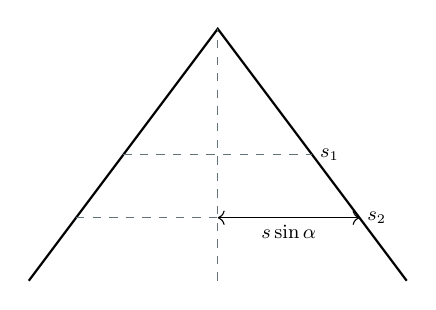
\begin{tikzpicture}[scale=.8,transform shape]
\draw[thick] (0,0)--(3,4)--(6,0);\draw[guide] (1.5,2)--(4.5,2);\draw[guide] (.75,1)--(5.25,1);\draw[guide] (3,0)--(3,4);\draw[<->] (3,1)--(5.25,1) node[midway,below] {$s\sin\alpha$};\node[right] at (4.5,2) {$s_1$};\node[right] at (5.25,1) {$s_2$};
\end{tikzpicture}
\figcaption{变图电试3.1V4\quad 圆锥面沿母线的长度与同心圆周宽度}
\end{minipage}\end{center}

\Needspace{20\baselineskip}
\item 两个环面片电阻率为$\rho^*(r)=\rho_0r/R_2$，柱面片电阻率为$\rho_0$，求总电阻。
\textbf{解：}变图电试3.1V5的环面每个径向条带有$\mathrm dR=\rho_0r\mathrm dr/(R_2\,2\pi r)=\rho_0\mathrm dr/(2\pi R_2)$，半径因子约去，所以每个环面电阻为$\rho_0(R_2-R_1)/(2\pi R_2)$。再加柱面项$\rho_0H/(2\pi R_2)$，得到$R=\rho_0[2(R_2-R_1)+H]/(2\pi R_2)$。电阻率随半径增大，抵消了圆周宽度随半径增大的效应，累计环面电势降变为线性。
\begin{center}\begin{minipage}{.98\linewidth}\centering
\begin{tikzpicture}[scale=.8,transform shape]
\draw[axis] (0,0)--(10.7,0) node[right] {$r/R_1$};
\draw[axis] (0,0)--(0,3.2) node[above] {$\rho^*/\rho_0$};\foreach \y/\lab in {0/0,1.4/0.5,2.8/1}{\draw[thin] (0,\y)--(-.08,\y) node[left] {$\lab$};}
\node[above] at (5,3.5) {$R_2/R_1=2$时电阻率沿半径线性增加};
\draw[traj] plot coordinates {(0.000000000,1.400000000) (0.083333333,1.411666667) (0.166666667,1.423333333) (0.250000000,1.435000000) (0.333333333,1.446666667) (0.416666667,1.458333333) (0.500000000,1.470000000) (0.583333333,1.481666667) (0.666666667,1.493333333) (0.750000000,1.505000000) (0.833333333,1.516666667) (0.916666667,1.528333333) (1.000000000,1.540000000) (1.083333333,1.551666667) (1.166666667,1.563333333) (1.250000000,1.575000000) (1.333333333,1.586666667) (1.416666667,1.598333333) (1.500000000,1.610000000) (1.583333333,1.621666667) (1.666666667,1.633333333) (1.750000000,1.645000000) (1.833333333,1.656666667) (1.916666667,1.668333333) (2.000000000,1.680000000) (2.083333333,1.691666667) (2.166666667,1.703333333) (2.250000000,1.715000000) (2.333333333,1.726666667) (2.416666667,1.738333333) (2.500000000,1.750000000) (2.583333333,1.761666667) (2.666666667,1.773333333) (2.750000000,1.785000000) (2.833333333,1.796666667) (2.916666667,1.808333333) (3.000000000,1.820000000) (3.083333333,1.831666667) (3.166666667,1.843333333) (3.250000000,1.855000000) (3.333333333,1.866666667) (3.416666667,1.878333333) (3.500000000,1.890000000) (3.583333333,1.901666667) (3.666666667,1.913333333) (3.750000000,1.925000000) (3.833333333,1.936666667) (3.916666667,1.948333333) (4.000000000,1.960000000) (4.083333333,1.971666667) (4.166666667,1.983333333) (4.250000000,1.995000000) (4.333333333,2.006666667) (4.416666667,2.018333333) (4.500000000,2.030000000) (4.583333333,2.041666667) (4.666666667,2.053333333) (4.750000000,2.065000000) (4.833333333,2.076666667) (4.916666667,2.088333333) (5.000000000,2.100000000) (5.083333333,2.111666667) (5.166666667,2.123333333) (5.250000000,2.135000000) (5.333333333,2.146666667) (5.416666667,2.158333333) (5.500000000,2.170000000) (5.583333333,2.181666667) (5.666666667,2.193333333) (5.750000000,2.205000000) (5.833333333,2.216666667) (5.916666667,2.228333333) (6.000000000,2.240000000) (6.083333333,2.251666667) (6.166666667,2.263333333) (6.250000000,2.275000000) (6.333333333,2.286666667) (6.416666667,2.298333333) (6.500000000,2.310000000) (6.583333333,2.321666667) (6.666666667,2.333333333) (6.750000000,2.345000000) (6.833333333,2.356666667) (6.916666667,2.368333333) (7.000000000,2.380000000) (7.083333333,2.391666667) (7.166666667,2.403333333) (7.250000000,2.415000000) (7.333333333,2.426666667) (7.416666667,2.438333333) (7.500000000,2.450000000) (7.583333333,2.461666667) (7.666666667,2.473333333) (7.750000000,2.485000000) (7.833333333,2.496666667) (7.916666667,2.508333333) (8.000000000,2.520000000) (8.083333333,2.531666667) (8.166666667,2.543333333) (8.250000000,2.555000000) (8.333333333,2.566666667) (8.416666667,2.578333333) (8.500000000,2.590000000) (8.583333333,2.601666667) (8.666666667,2.613333333) (8.750000000,2.625000000) (8.833333333,2.636666667) (8.916666667,2.648333333) (9.000000000,2.660000000) (9.083333333,2.671666667) (9.166666667,2.683333333) (9.250000000,2.695000000) (9.333333333,2.706666667) (9.416666667,2.718333333) (9.500000000,2.730000000) (9.583333333,2.741666667) (9.666666667,2.753333333) (9.750000000,2.765000000) (9.833333333,2.776666667) (9.916666667,2.788333333) (10.000000000,2.800000000)};
\node[below] at (0,-.12) {$1$};
\node[below] at (10,-.12) {$2$};
\end{tikzpicture}
\figcaption{变图电试3.1V5\quad $R_2/R_1=2$时电阻率沿半径线性增加}
\end{minipage}\end{center}

\Needspace{20\baselineskip}
\item 另加一条同片电阻率的内圆柱面，直接连接上下内圆周，求两端口间等效电阻。
\textbf{解：}变图电试3.1V6中已有外侧路径电阻记为$R_o=(\rho^*/\pi)[\ln(R_2/R_1)+H/(2R_2)]$。新增内柱面长$H$、宽$2\pi R_1$，电阻$R_i=\rho^*H/(2\pi R_1)$。两条路径只在同一对内圆周端口连接，端电压相同，故并联电阻为$R_oR_i/(R_o+R_i)$。总电流分别按$\Delta U/R_o$和$\Delta U/R_i$分流，新增导电面改变的是两端口之间的连接关系。
\begin{center}\begin{minipage}{.98\linewidth}\centering
\begin{tikzpicture}[scale=.8,transform shape]
\node[draw] (a) at (0,1) {上内圈};\node[draw] (b) at (6,1) {下内圈};\draw (a)--(1.5,1)--(1.5,2.2)--(4.5,2.2)--(4.5,1)--(b);\draw (1.5,1)--(1.5,-.2)--(4.5,-.2)--(4.5,1);\node[above] at (3,2.2) {$R_o$外侧三段};\node[below] at (3,-.2) {$R_i$内柱面};
\end{tikzpicture}
\figcaption{变图电试3.1V6\quad 新增内柱面连接同一对端口，形成并联路径}
\end{minipage}\end{center}

\Needspace{20\baselineskip}
\item 固定$R_1,H,\rho^*$，改变外半径$R_2>R_1$，求总电阻最小的几何条件。
\textbf{解：}变图电试3.1V7对$R=(\rho^*/\pi)[\ln(R_2/R_1)+H/(2R_2)]$求导，得$\mathrm dR/\mathrm dR_2=(\rho^*/\pi)(2R_2-H)/(2R_2^2)$。当$H>2R_1$，导数在$R_2=H/2$由负变正，得到唯一最小值；当$H\le2R_1$，允许区间内导数为正，电阻随$R_2$增加，最小下确界在$R_2\to R_1^+$。增大外半径会增加两环面的路径长度，同时增大柱面的导电宽度。图中 $H/R_1=5$ 的实心点横坐标为 $5/2$，纵坐标为 $1+\ln(5/2)$；左端空心点表示模型只取 $R_2>R_1$。在 $H\le 2R_1$ 时只有左端的下确界，值为 $\rho^*H/(2\pi R_1)$。
\begin{center}\begin{minipage}{.98\linewidth}\centering
\begin{tikzpicture}[x=1.4cm,y=3.65cm,font=\small]
\draw[axis] (1,1.78)--(5.3,1.78) node[right] {$R_2/R_1$};
\draw[axis] (1,1.78)--(1,2.63) node[above] {$\pi R_{\rm eq}/\rho^*$};
\foreach \x/\lab in {1/1,2.5/2.5,5/5}{
 \draw[object] (\x,1.78)--(\x,1.761) node[below] {$\lab$};
}
\foreach \y in {1.9,2.2,2.5}{
 \draw[object] (1,\y)--(.95,\y) node[left] {$\y$};
}
\draw[traj,domain=1:5,samples=93] plot (\x,{ln(\x)+2.5/\x});
\draw[guide] (2.5,1.78)--(2.5,1.916291);
\draw[traj,fill=white] (1,2.5) circle(1.6pt);
\fill[warm] (2.5,1.916291) circle(1.7pt) node[above right] {极小值};
\node[above] at (4.56,2.49) {$H/R_1=5$};
\end{tikzpicture}
\figcaption{变图电试3.1V7\quad 纵轴放大极小值附近；曲线最低处的实心点对应 $R_2=H/2$。}
\end{minipage}\end{center}

\Needspace{20\baselineskip}
\item 求上环面的局部焦耳功率密度，并由总耗散再次求几何电阻。
\textbf{解：}变图电试3.1V8中单位面积耗散为$p_s=\boldsymbol j^*\cdot\boldsymbol E=\rho^*I^2/(4\pi^2r^2)$。径向宽度$\mathrm dr$的环带面积$2\pi r\mathrm dr$，所以其功率为$\rho^*I^2\mathrm dr/(2\pi r)$；两环面相加，再加柱面功率$\rho^*I^2H/(2\pi R_2)$，总功率为$I^2R_{\rm eq}$。内缘与外缘的单位面积功率密度比为$(R_2/R_1)^2$，展示径向电流在较窄圆周处的集中效应。
\begin{center}\begin{minipage}{.98\linewidth}\centering
\begin{tikzpicture}[scale=.8,transform shape]
\draw[axis] (0,0)--(10.7,0) node[right] {$r/R_1$};
\draw[axis] (0,0)--(0,3.2) node[above] {$p_s/p_s(R_1)$};\foreach \y/\lab in {0/0,1.4/0.5,2.8/1}{\draw[thin] (0,\y)--(-.08,\y) node[left] {$\lab$};}
\node[above] at (5,3.5) {环面电流集中使内圆周附近的单位面积耗散较大};
\draw[traj] plot coordinates {(0.000000000,2.800000000) (0.083333333,2.753910252) (0.166666667,2.708949207) (0.250000000,2.665080309) (0.333333333,2.622268470) (0.416666667,2.580480000) (0.500000000,2.539682540) (0.583333333,2.499845000) (0.666666667,2.460937500) (0.750000000,2.422931314) (0.833333333,2.385798817) (0.916666667,2.349513432) (1.000000000,2.314049587) (1.083333333,2.279382667) (1.166666667,2.245488973) (1.250000000,2.212345679) (1.333333333,2.179930796) (1.416666667,2.148223134) (1.500000000,2.117202268) (1.583333333,2.086848507) (1.666666667,2.057142857) (1.750000000,2.028066999) (1.833333333,1.999603253) (1.916666667,1.971734559) (2.000000000,1.944444444) (2.083333333,1.917717004) (2.166666667,1.891536874) (2.250000000,1.865889213) (2.333333333,1.840759679) (2.416666667,1.816134408) (2.500000000,1.792000000) (2.583333333,1.768343494) (2.666666667,1.745152355) (2.750000000,1.722414456) (2.833333333,1.700118064) (2.916666667,1.678251821) (3.000000000,1.656804734) (3.083333333,1.635766157) (3.166666667,1.615125781) (3.250000000,1.594873621) (3.333333333,1.575000000) (3.416666667,1.555495544) (3.500000000,1.536351166) (3.583333333,1.517558056) (3.666666667,1.499107674) (3.750000000,1.480991736) (3.833333333,1.463202206) (3.916666667,1.445731292) (4.000000000,1.428571429) (4.083333333,1.411715276) (4.166666667,1.395155709) (4.250000000,1.378885811) (4.333333333,1.362898864) (4.416666667,1.347188346) (4.500000000,1.331747919) (4.583333333,1.316571429) (4.666666667,1.301652893) (4.750000000,1.286986498) (4.833333333,1.272566595) (4.916666667,1.258387691) (5.000000000,1.244444444) (5.083333333,1.230731663) (5.166666667,1.217244294) (5.250000000,1.203977425) (5.333333333,1.190926276) (5.416666667,1.178086194) (5.500000000,1.165452653) (5.583333333,1.153021247) (5.666666667,1.140787687) (5.750000000,1.128747795) (5.833333333,1.116897507) (5.916666667,1.105232861) (6.000000000,1.093750000) (6.083333333,1.082445166) (6.166666667,1.071314699) (6.250000000,1.060355030) (6.333333333,1.049562682) (6.416666667,1.038934268) (6.500000000,1.028466483) (6.583333333,1.018156107) (6.666666667,1.008000000) (6.750000000,0.997995099) (6.833333333,0.988138418) (6.916666667,0.978427043) (7.000000000,0.968858131) (7.083333333,0.959428911) (7.166666667,0.950136676) (7.250000000,0.940978786) (7.333333333,0.931952663) (7.416666667,0.923055791) (7.500000000,0.914285714) (7.583333333,0.905640035) (7.666666667,0.897116412) (7.750000000,0.888712557) (7.833333333,0.880426238) (7.916666667,0.872255273) (8.000000000,0.864197531) (8.083333333,0.856250929) (8.166666667,0.848413433) (8.250000000,0.840683055) (8.333333333,0.833057851) (8.416666667,0.825535923) (8.500000000,0.818115413) (8.583333333,0.810794506) (8.666666667,0.803571429) (8.750000000,0.796444444) (8.833333333,0.789411857) (8.916666667,0.782472006) (9.000000000,0.775623269) (9.083333333,0.768864057) (9.166666667,0.762192817) (9.250000000,0.755608028) (9.333333333,0.749108205) (9.416666667,0.742691890) (9.500000000,0.736357659) (9.583333333,0.730104120) (9.666666667,0.723929905) (9.750000000,0.717833680) (9.833333333,0.711814137) (9.916666667,0.705869995) (10.000000000,0.700000000)};
\node[below] at (0,-.12) {$1$};
\node[below] at (10,-.12) {$2$};
\end{tikzpicture}
\figcaption{变图电试3.1V8\quad 环面电流集中使内圆周附近的单位面积耗散较大}
\end{minipage}\end{center}
\end{enumerate}

\Needspace{13\baselineskip}

\pdfbookmark[2]{第 2 题 双环网络与无限内接正方形网络}{q2}

\section*{第 2 题\quad 双环网络与无限内接正方形网络}\label{q:2}


\begin{enumerate}
\item 两同心圆各在上、右、下、左四个方位设置结点，并以四条径向线段连接内外对应结点。每一四分之一圆弧及每一径向线段的电阻均为$r$。求外圆下方结点$A$与内圆右方结点$B$之间的等效电阻，给出必要中间结果。
\item 从正方形$ABCD$开始，不断连接相邻边中点构成内接正方形；各层边与相接的中点均为电连接。所有金属丝材料、粗细相同，最外层每边电阻为$R_0$。$A,B,C,D$依次为上、左、下、右顶点，第一内接正方形的上左、下左、下右、上右顶点依次为$E,F,G,J$；再内一层的上、下顶点为$H,I$。求$R_{AC}$与$R_{EG}$。
\end{enumerate}
无限网络的等效电阻按保留有限层、最内层不再接入支路后的极限定义。


\begin{center}\begin{minipage}{.98\linewidth}\centering
\begin{tikzpicture}[scale=.65,transform shape]

\draw[object] (0,0) circle (2);\draw[object] (0,0) circle (1);
\foreach \a in {0,90,180,270}{\draw[object] (\a:1)--(\a:2);}
\fill (0,-2) circle (1.7pt) node[below] {$A$};
\fill (1,0) circle (1.7pt) node[above right] {$B$};
\fill (0,-1) circle (1.7pt) node[above left] {$C_0$};
\node at (0,2.5) {每段电阻$r$};
\begin{scope}[xshift=7.5cm]
\foreach \k in {0,...,7}{
\pgfmathsetmacro{\rr}{2.8*pow(.7071067812,\k)}
\pgfmathsetmacro{\ang}{90+45*\k}
\draw[object] ({\rr*cos(\ang)},{\rr*sin(\ang)})--
({\rr*cos(\ang+90)},{\rr*sin(\ang+90)})--
({\rr*cos(\ang+180)},{\rr*sin(\ang+180)})--
({\rr*cos(\ang+270)},{\rr*sin(\ang+270)})--cycle;}
\node[above] at (0,2.8) {$A$};\node[left] at (-2.8,0) {$B$};
\node[below] at (0,-2.8) {$C$};\node[right] at (2.8,0) {$D$};
\node[above left] at (-1.4,1.4) {$E$};
\node[below left] at (-1.4,-1.4) {$F$};
\node[below right] at (1.4,-1.4) {$G$};
\node[above right] at (1.4,1.4) {$J$};
\node[above] at (0,1.4) {$H$};\node[below] at (0,-1.4) {$I$};
\node at (0,-3.5) {同材料同粗细；各层中点相连};
\end{scope}
\end{tikzpicture}
\figcaption{图电试3.2\quad 左侧双环四辐条，右侧无限内接正方形，各题按给定端口求电阻。}
\end{minipage}\end{center}

\Needspace{8\baselineskip}

\pdfbookmark[3]{题型定位}{q2-h0}

\subsection*{题型定位}

有限网络先利用电流叠加和等势变形，再以无限内接网络的比例结构建立递推。端口激励决定电势对称性，几何连接决定可合并或拆开的结点。有限双环与立方体十二棱保持同一连接图，无限正方形则按相同材料、粗细的线长缩放电阻，最终用有限截断的收敛选定正固定点。

\Needspace{8\baselineskip}

\pdfbookmark[3]{知识点}{q2-h1}

\subsection*{知识点}

外加电流在稳恒线性网络中可以叠加，支路电流保留参考方向的正负。等势结点间的支路无电流，对称折叠后的重合支路并联。图同构保留结点和支路的连接关系，端口也随映射对应。内接正方形隔一层的线度为$1/\sqrt2$，隔两层的同向对角线为$1/2$。无限网络的正电阻递推与有限层开端截断共同给出唯一极限。

\Needspace{8\baselineskip}

\pdfbookmark[3]{物理图像}{q2-h2}

\subsection*{物理图像}

题图的双环有八个结点、十二个支路；各层正方形的中点都与下一层顶点相接。解图电试3.2A保留两组激励中支路的有符号电流，图B把等势支路折叠成并联。图C框出$HI$内侧的同类网络并标$X/2$，图D将$EG$重新表示为三条端口相同的通道。图E用有限层数的实际电阻显示两个端口对的收敛。

\Needspace{8\baselineskip}

\pdfbookmark[3]{解题入口}{q2-h3}

\subsection*{解题入口}

第一问取电压路径$A\to C_0\to B$，把原激励拆成两组具有对称性的外加电流，先求一组电势再用拓扑置换得到另一组。第二问在$AC$激励下先确定对称折叠，标出$a,b,d$各自对应的金属丝，将$HI$内侧的同类网络以$R_{HI}=X/2$代入。求$EG$时换用该端口条件的对称性，把外圈两条通路和第一内层整体分别保留。

\Needspace{8\baselineskip}

\pdfbookmark[3]{标准解法}{q2-h4}

\subsection*{标准解法}


图电试3.2左侧是八结点、十二支路网络，右侧各层每缩小一层，边长和单边电阻都乘$1/\sqrt2$。两小问分别利用电流叠加与网络自相似，结点按相同端口激励下的电势关系确定合并或拆开。

第（1）问，记内圆下方结点为$C_0$，支路$AC_0$、$C_0B$都各为$r$。给定电流$I$从$A$流入、$B$流出，端电压可沿这两支路计算：
\[
R_{AB}=r\frac{I_{AC_0}+I_{C_0B}}{I}.
\]
将这一电流分布叠加为两组：第一组$I$从$A$入、$C_0$出；第二组$I$从$C_0$入、$B$出，中间结点的外加电流正好抵消。
\begin{center}\begin{minipage}{.98\linewidth}\centering
\begin{tikzpicture}[scale=.75,transform shape]

\draw[object] (0,0) circle (2);\draw[object] (0,0) circle (1);
\foreach \a in {0,90,180,270}{\draw[object] (\a:1)--(\a:2);}
\fill (0,-2) circle (1.7pt) node[below right] {$A$};
\fill (1,0) circle (1.7pt) node[above right] {$B$};
\fill (0,-1) circle (1.7pt) node[above left] {$C_0$};
\node at (0,2.5) {每段电阻$r$};

\draw[motion] (0,-3)--(0,-2.2) node[midway,left] {$I$};
\draw[motion] (-.1,-1.1)--(-.8,-1.5) node[left] {$I$流出};
\draw[force] (.14,-1.85)--(.14,-1.2) node[right] {$I_{AC_0}$};
\draw[force] (-60:1.15) arc[start angle=-60,end angle=-20,radius=1.15];
\node[right] at (1.2,-1.5) {$I_{C_0B}$};
\node[align=left] at (5,1) {第一组：$A$入、$C_0$出\\$I_{AC_0}^{(1)}=7I/12$\\$I_{C_0B}^{(1)}=-5I/24$};
\node[align=left] at (5,-1.3) {第二组：$C_0$入、$B$出\\$I_{AC_0}^{(2)}=-5I/24$\\$I_{C_0B}^{(2)}=7I/12$};

\end{tikzpicture}
\figcaption{解图电试3.2A\quad 两组外加电流在中间端口抵消，支路代数电流按同一箭头叠加。}
\end{minipage}\end{center}
解图电试3.2A中第一组关于竖直直径对称。以$Ir$为电势单位、$V_{C_0}=0$，记$A$、外圆右左、外圆上、内圆右左、内圆上这五类结点电势分别为$a,b,c,d,f$。结点方程为
\[
\begin{gathered}
3a-2b=1,\quad a+2d=1,\quad
3b-a-c-d=0,\\
3c-2b-f=0,\quad
3d-b-f=0,\quad 3f-2d-c=0.
\end{gathered}
\]
每个结点都接三条阻值$r$的支路，结点电势乘3后减去三个相邻电势就是外加电流乘$r$。竖直直径对称使左右成对电势相等，因此$b,d$各代表两个结点，方程中相应出现系数2。第二式是流出端$C_0$的电流条件。解得
\[
(a,b,c,d,f)=\left(\frac7{12},\frac38,\frac13,
\frac5{24},\frac14\right).
\]
例如$a+2d=7/12+2(5/24)=1$，表示三条流向$C_0$的电流总和等于$I$；$3a-2b=1$则是$A$点外加电流的条件。$C_0\to B$规定的参考方向从零电势指向$d=5/24$，所以该支路第一组电流为负。通过外加电流叠加，两组在$C_0$端的流入、流出互相抵消，而A、B端保留题设激励。所以第一组中
\[
I_{AC_0}^{(1)}=\frac7{12}I,\qquad
I_{C_0B}^{(1)}=-\frac5{24}I.
\]
第二组由同一十二支路拓扑的对称置换，可得
\[
I_{AC_0}^{(2)}=-\frac5{24}I,\qquad
I_{C_0B}^{(2)}=\frac7{12}I.
\]
两组相加，$I_{AC_0}=I_{C_0B}=3I/8$，因此
\[
\boxed{R_{AB}=\frac34r}.
\]
\begin{center}\begin{minipage}{.98\linewidth}\centering
\begin{tikzpicture}[scale=.75,transform shape]

\draw[object] (0,0)--(0,2) node[midway,left] {$r$};
\draw[object] (4,0)--(4,2) node[midway,right] {$r$};
\draw[object] (0,0)--(2,0) node[midway,below] {$r/2$};
\draw[object] (2,0)--(4,0) node[midway,below] {$r/2$};
\draw[object] (0,2)--(2,2) node[midway,above] {$r/2$};
\draw[object] (2,2)--(4,2) node[midway,above] {$r/2$};
\draw[guide] (2,0)--(2,2) node[midway,right] {$r/2$};
\node[below left] at (0,0) {$A$};\node[below right] at (4,0) {$B$};
\node at (2,3.1) {等势折叠后，桥支路无电流};
\begin{scope}[xshift=6cm]
\draw[object] (0,0)--(0,2)--(3,2)--(3,0)--cycle;
\node[fill=white] at (1.5,2) {$3r$};
\node[fill=white] at (1.5,0) {$r$};
\node[below left] at (0,0) {$A$};\node[below right] at (3,0) {$B$};
\node at (1.5,-1) {$r\parallel3r=3r/4$};
\end{scope}

\end{tikzpicture}
\figcaption{解图电试3.2B\quad 与立方体面对角端口同构的折叠网络，删除桥支路后只余两通路。}
\end{minipage}\end{center}
解图电试3.2B给出立方体等势变形：两圆上的各四个结点对应立方体的两个四边形面，四条辐条对应连接两面的四条棱，十二条电阻一一保留。$A,B$对应立方体同一面的相对顶点，沿棱连接时相隔两条棱。关于通过这两个端点的对称面折叠后，成对支路并联为$r/2$，中间桥支路两端等势而无电流。去掉桥支路，得到$r$与$3r$并联，仍为$3r/4$。折叠只合并已由对称性证明等势的结点。

立方体变形中，每一条弧段对应一条棱，原来四条辐条对应两个四边形面之间的四条连接棱，因此总支路仍为十二条。等势折叠只把对称支路并联，几何图可以拉伸、转动，电阻连接和端口位置关系保持。对折叠后无电流桥支路的删除，则使用该对端口下的等势条件。

第（2）问先求$X=R_{AC}$。取$V_A=U,V_C=0$，关于$BD$反射会交换两端；由结点方程的唯一性，反射位置的电势为$U-V$。$BD$上的结点在反射下保持原位，电势因而同为$U/2$。再利用关于$AC$的左右反射，两侧对应结点等势，可沿$AC$折叠，把两侧相同电阻并联。记
\[
a=\frac{R_0}{4},\qquad
b=\frac{\sqrt2R_0}{8},\qquad
d=\frac{2ab}{a+b}.
\]
这里$a$是外层半边折叠后的电阻，$b$是第一内层半边折叠后的电阻；折叠后仍保留中心以内的网络。
\begin{center}\begin{minipage}{.98\linewidth}\centering
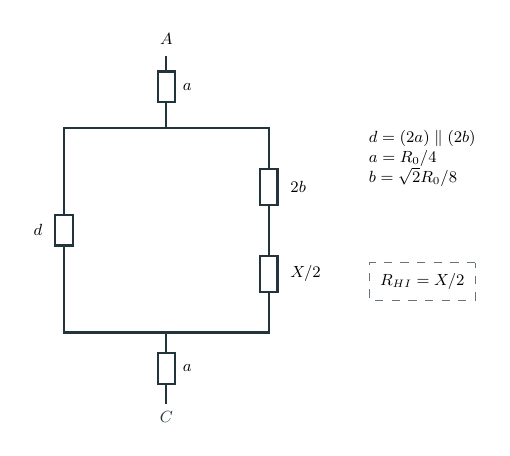
\begin{tikzpicture}[scale=.65,transform shape]

\node[above] at (0,4.5) {$A$};
\draw[object] (0,4.4)--(0,4.1);
\draw[object] (-.17,3.5) rectangle (.17,4.1);\node[right] at (.2,3.8) {$a$};
\draw[object] (0,3.5)--(0,3)--(-2,3)--(-2,1.3);
\draw[object] (-2.17,.7) rectangle (-1.83,1.3);\node[left] at (-2.3,1) {$d$};
\draw[object] (-2,.7)--(-2,-1)--(2,-1)--(2,-.2);
\draw[object] (1.83,-.2) rectangle (2.17,.5);\node[right] at (2.3,.15) {$X/2$};
\draw[object] (2,.5)--(2,1.5);
\draw[object] (1.83,1.5) rectangle (2.17,2.2);\node[right] at (2.3,1.85) {$2b$};
\draw[object] (2,2.2)--(2,3)--(0,3);
\draw[object] (0,-1)--(0,-1.4);
\draw[object] (-.17,-2) rectangle (.17,-1.4);\node[right] at (.2,-1.7) {$a$};
\draw[object] (0,-2)--(0,-2.4) node[below] {$C$};
\node[align=left] at (5,2.4) {$d=(2a)\parallel(2b)$\\$a=R_0/4$\\$b=\sqrt2R_0/8$};
\node[draw=muted,dashed,inner sep=6pt] at (5,0) {$R_{HI}=X/2$};

\end{tikzpicture}
\figcaption{解图电试3.2C\quad AC折叠等效中，内层同向对角线电阻为X的一半。}
\end{minipage}\end{center}
解图电试3.2C中，在两端串联的$a$之间，有两组并联通道：左侧外支路$2a$与中间支路$2b$先并联成$d$，右侧通道为$2b+R_{HI}$。$HI$相对于$AC$是隔两层的同向对角线，线性尺度减半，故$R_{HI}=X/2$。外层半边长对应$R_0/2$，折叠把左右两条这样的支路并联，得到$a=R_0/4$。第一内层边长是外层的$1/\sqrt2$，其半边再折叠给$b=R_0/(4\sqrt2)$。$HI$间内网络跨过两次缩放，端口方向重新与$AC$相同，因此整体电阻为$X/2$。先并联$2a$与$2b$得到$d$，再将它与$2b+X/2$并联，最后串联两端$a$。于是
\[
\boxed{X=2a+\frac{d(2b+X/2)}{d+2b+X/2}}.
\]
令$t=X/(2b)$，利用$a=\sqrt2b$、$d=2(2-\sqrt2)b$，化为
\[
t^2+(4-2\sqrt2)t-4\sqrt2=0.
\]
从递推式移去两端的$2a$，再乘并联分母，得到关于$X$的二次方程。归一化为$t=X/(2b)$后，常数项为负，说明两根异号；正电阻对应其中正的根。两根中只有正根可作电阻，故
\[
t=\sqrt6+\sqrt2-2,\qquad
\boxed{R_{AC}=\frac{\sqrt3+1-\sqrt2}{2}R_0}.
\]
递推右边对$X$的导数为
\[
\frac{d^2}{2(d+2b+X/2)^2}<\frac12\quad(X\ge0).
\]
所以不同有限层终端的影响逐层衰减，正固定点为有限截断网络的唯一极限，其数值由给定的有限截断定义唯一确定。
\begin{center}\begin{minipage}{.98\linewidth}\centering
\begin{tikzpicture}[scale=.85,transform shape]

\draw[object] (0,0)--(0,1.7)--(5,1.7)--(5,-1.7)--(0,-1.7)--(0,0);
\draw[object] (0,0)--(5,0);
\node[draw=ink,fill=white,minimum width=1.5cm,minimum height=.45cm] at (2.5,1.7) {$2R_0$};
\node[draw=ink,fill=white,minimum width=1.5cm,minimum height=.45cm] at (2.5,0) {$X/\sqrt2$};
\node[draw=ink,fill=white,minimum width=1.5cm,minimum height=.45cm] at (2.5,-1.7) {$2R_0$};
\draw[motion] (-1,0)--(-.1,0);\draw[motion] (5.1,0)--(6,0);
\node[above left] at (0,0) {$E$};\node[above right] at (5,0) {$G$};
\node at (2.5,2.6) {外圈通路、内侧网络、外圈通路并联};

\end{tikzpicture}
\figcaption{解图电试3.2D\quad EG端口的内侧与AC网络相似、尺度缩小一层，外围另有两条通路。}
\end{minipage}\end{center}
\begin{center}\begin{minipage}{.98\linewidth}\centering
\begin{tikzpicture}[scale=.8,transform shape]
\draw[axis] (0,0)--(10.7,0) node[right] {内接层数$N$};
\draw[axis] (0,0)--(0,3.2) node[above] {$R/R_0$};\foreach \y/\lab in {0/0,1.2/0.3,2.4/0.6}{\draw[thin] (0,\y)--(-.08,\y) node[left] {$\lab$};}
\node[above] at (5,3.5) {实线$AC$，虚线$EG$；有限层逐渐趋于无限极限};
\draw[traj] plot coordinates {(0.000000000,2.828427125) (0.909090909,2.666666667) (1.818181818,2.640754482) (2.727272727,2.636509763) (3.636363636,2.635811899) (4.545454545,2.635697097) (5.454545455,2.635678210) (6.363636364,2.635675102) (7.272727273,2.635674591) (8.181818182,2.635674507) (9.090909091,2.635674493) (10.000000000,2.635674491)};
\draw[dashed,thick,color=warm] plot coordinates {(0.000000000,1.656854249) (0.909090909,1.333333333) (1.818181818,1.281508964) (2.727272727,1.273019525) (3.636363636,1.271623799) (4.545454545,1.271394194) (5.454545455,1.271356420) (6.363636364,1.271350205) (7.272727273,1.271349182) (8.181818182,1.271349014) (9.090909091,1.271348986) (10.000000000,1.271348982)};
\node[below] at (0,-.12) {$1$};
\node[below] at (4.545454545454546,-.12) {$6$};
\node[below] at (10,-.12) {$12$};
\end{tikzpicture}
\figcaption{解图电试3.2E\quad 实线$AC$，虚线$EG$；有限层逐渐趋于无限极限}
\end{minipage}\end{center}
图E的每个有限层都在最内层保留完整正方形，且不再接入更深支路；两组曲线按相同截断方式得到。只保留外层时$R_{AC}^{(0)}=R_0$，保留第一内层时$R_{AC}^{(1)}=R_0/\sqrt2$。后续隔两层用同一递推更新，新增导线使端口电阻不增加，递推导数的上界则控制远端截断的影响，二者共同确定题设的无限极限。

再求$R_{EG}$。解图电试3.2D中，外层从$E$到$G$有两条各为$2R_0$的通路；内侧是以第一内接正方形为外边界的同类网络，$E,G$为其对角端点，电阻为$X/\sqrt2$。关于$FJ$反射会交换$E,G$，而$F,J$保持原位，故$F,J$均在两端平均电势上，各部分在这两点无净交换电流，可将这些等势结点拆开，三通道因而并联：
\[
\frac1{R_{EG}}=\frac1{2R_0}+\frac1{2R_0}
+\frac1{X/\sqrt2}
=\frac1{R_0}+\frac{\sqrt2}{X}.
\]
外侧两条路径分别经过外正方形上、右顶点与左、下顶点，每条包含四段半边，故电阻均为$2R_0$。内侧第一正方形的$E,G$是对角端口，线阻按其整体尺寸缩为$X/\sqrt2$。拆开$F,J$时，各子网络在这两个平均电势点的净交换电流为零，所以端口电流恰为三通道电流之和。代入$X$并有理化，
\[
\boxed{R_{EG}=(\sqrt3-\sqrt2)R_0}.
\]
两个结果都随$R_0$线性缩放；$R_{EG}<R_{AC}<R_0$也与可用通路和正电阻网络的单调性相符。


\Needspace{8\baselineskip}

\pdfbookmark[3]{关键洞察}{q2-h5}

\subsection*{关键洞察}

同一网络换一对端口，等势结点集合也随激励改变。立方体映射的物理内容是十二条电阻的连接保持，视觉距离不参与计算。无限图的几何比例与同材料线阻关系结合，才形成电阻比例；同向内层对角线跨两层，$EG$所接内网络则只缩一层。

\Needspace{8\baselineskip}

\pdfbookmark[3]{易错点}{q2-h6}

\subsection*{易错点}

双环的指定端点映射为立方体同面相对顶点，按两条棱的距离识别。叠加支路电流时保留负号，折叠后成对电阻按并联减半。$HI$与$AC$的尺度比为$1/2$，$EG$内网络与$AC$整体的尺度比为$1/\sqrt2$，各自对应不同几何对象。固定点取正根，并由有限截断递推说明极限；$EG$还包括两条外圈路径。

\Needspace{8\baselineskip}

\pdfbookmark[3]{课堂讲解建议}{q2-h7}

\subsection*{课堂讲解建议}

先给双环八个结点编号，把两圆分别画成立方体两面，逐条保持十二个支路。利用第一组电势表解释负支路电流，再把两组外加激励相加。折叠法则先画等势桥两端的电势，再移去该支路。

进入无限网络，要求在几何图上圈出$HI$内侧的完整同类图，再按线长给比例。将递推按串联、并联逐层写出，求根后用有限层数图说明终端影响怎样衰减。最后为$EG$重新画三个通道，让学生逐一说出路径、电阻和端口，把两种端口激励下各自保留的路径与电阻比例连起来。

\Needspace{8\baselineskip}

\pdfbookmark[3]{变式训练}{q2-h8}

\subsection*{变式训练}

\begin{enumerate}
\Needspace{20\baselineskip}
\item 把双环端口改为外圆下点$A$与内圆下点$C_0$，求等效电阻。
\textbf{解：}变图电试3.2V1的两端是同一辐条的端点，对应立方体相邻顶点。第一组电势表在$V_{C_0}=0$时给$V_A=7Ir/12$，因此$R_{AC_0}=7r/12$。总电流的一部分沿直接辐条流动，其余从两侧圆弧绕行；辐条电流为$7I/12$，其他路径合计$5I/12$。端口改变后使用这一组激励，原来叠加后的$3r/4$属于另一对端点。
\begin{center}\begin{minipage}{.98\linewidth}\centering
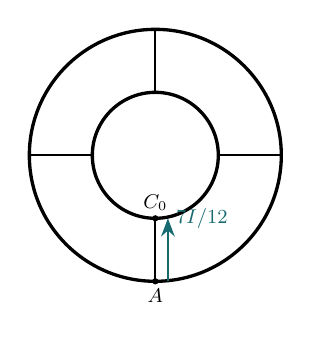
\begin{tikzpicture}[scale=.8,transform shape]
\draw[very thick] (0,0) circle (2);\draw[very thick] (0,0) circle (1);\foreach \a in {0,90,180,270}{\draw[thick] (\a:1)--(\a:2);}\fill (0,-2) circle(.05) node[below] {$A$};\fill (0,-1) circle(.05) node[above] {$C_0$};\draw[motion] (.2,-2)--(.2,-1) node[right] {$7I/12$};
\end{tikzpicture}
\figcaption{变图电试3.2V1\quad 同一辐条端点对应立方体相邻顶点}
\end{minipage}\end{center}

\Needspace{20\baselineskip}
\item 把立方体网络的端口改为体对角顶点，求电阻并说明等势点分组。
\textbf{解：}变图电试3.2V2中输入端相邻的三个顶点由三重对称性等势，输出端相邻的三个顶点也等势。输入端到第一组有3条$r$并联，第一组到第二组有6条$r$并联，第二组到输出端也有3条$r$并联，三段串联给$r/3+r/6+r/3=5r/6$。双环原来的一对端口对应同面对角，其$3r/4$与这里的差别来自端口激励。
\begin{center}\begin{minipage}{.98\linewidth}\centering
\begin{tikzpicture}[scale=.8,transform shape]
\node[draw] (a) at (0,1) {$A$};\node[draw] (b) at (2.5,1) {第一等势组};\node[draw] (c) at (6,1) {第二等势组};\node[draw] (d) at (8.5,1) {$B$};\draw (a)--(b) node[midway,above] {$r/3$};\draw (b)--(c) node[midway,above] {$r/6$};\draw (c)--(d) node[midway,above] {$r/3$};
\end{tikzpicture}
\figcaption{变图电试3.2V2\quad 立方体体对角激励的三段串联等效}
\end{minipage}\end{center}

\Needspace{20\baselineskip}
\item 全部线阻统一乘$k$，或只改变最深处的有限终端，分别说明端口电阻怎样变化。
\textbf{解：}变图电试3.2V3中结点电流比例由电阻比决定，统一乘$k$使给定电流下全部电势差乘$k$，所以两端口电阻均乘$k$。若只使内层终端改变$\delta X$，同向隔层递推$F(X)$的导数为$d^2/[2(d+2b+X/2)^2]<1/2$，由中值定理，外层改变量小于$|\delta X|/2$。递推$n$次后小于$|\delta X|/2^n$，远处终端的影响逐层减弱。
\begin{center}\begin{minipage}{.98\linewidth}\centering
\begin{tikzpicture}[scale=.8,transform shape]
\draw[axis] (0,0)--(10.7,0) node[right] {同向隔层次数$n$};
\draw[axis] (0,0)--(0,3.2) node[above] {$|\delta X_n|/|\delta X_0|$上界};\foreach \y/\lab in {0/0,1.4/0.5,2.8/1}{\draw[thin] (0,\y)--(-.08,\y) node[left] {$\lab$};}
\node[above] at (5,3.5) {深层终端改变量逐层衰减};
\draw[traj] plot coordinates {(0.000000000,2.800000000) (1.250000000,1.400000000) (2.500000000,0.700000000) (3.750000000,0.350000000) (5.000000000,0.175000000) (6.250000000,0.087500000) (7.500000000,0.043750000) (8.750000000,0.021875000) (10.000000000,0.010937500)};
\node[below] at (0,-.12) {$0$};
\node[below] at (5,-.12) {$4$};
\node[below] at (10,-.12) {$8$};
\end{tikzpicture}
\figcaption{变图电试3.2V3\quad 深层终端改变量逐层衰减}
\end{minipage}\end{center}

\Needspace{20\baselineskip}
\item 只保留外层正方形，再逐层增加内接线，说明$R_{AC}$的单调性与上界。
\textbf{解：}变图电试3.2V4的初始网络只有两条各含两边的通路，$R_{AC}^{(0)}=(2R_0)\parallel(2R_0)=R_0$。每次加内接线都只增加正电导通路，固定端电压下总耗散的极小值增大、总电流增大，所以端口电阻不增加。有限层序列有正下界并趋于递推正固定点$(\sqrt3+1-\sqrt2)R_0/2$。这一上界与正电阻条件共同限定代数根。
\begin{center}\begin{minipage}{.98\linewidth}\centering
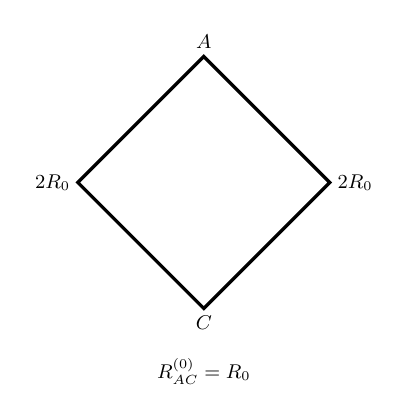
\begin{tikzpicture}[scale=.8,transform shape]
\draw[very thick] (0,2)--(-2,0)--(0,-2)--(2,0)--cycle;\node[above] at (0,2) {$A$};\node[below] at (0,-2) {$C$};\node[left] at (-2,0) {$2R_0$};\node[right] at (2,0) {$2R_0$};\node at (0,-3) {$R_{AC}^{(0)}=R_0$};
\end{tikzpicture}
\figcaption{变图电试3.2V4\quad 最外正方形提供有限层序列的初始上界}
\end{minipage}\end{center}

\Needspace{20\baselineskip}
\item 双环的八段圆弧仍为$r$，四根辐条改为$kr$，$k>0$，求指定端口$A,B$的电阻。
\textbf{解：}变图电试3.2V5取外环右、上、左、下四点的无量纲电势为$u_0,u_1,u_2,u_3$，内环相应为$v_0,v_1,v_2,v_3$，单位为$Ir$，并令$B$点$v_0=0$。下标按模4循环，结点方程为$(2+1/k)u_i-u_{i-1}-u_{i+1}-v_i/k=\delta_{i3}$与$(2+1/k)v_i-v_{i-1}-v_{i+1}-u_i/k=-\delta_{i0}$。消元得$u_0=k(k+2)/[4(k+1)]$、$u_2=(k+1)/4$、$v_3=3/8$。再由输入点方程$(2+1/k)u_3=1+u_0+u_2+v_3/k$得到$R_{AB}/r=(k+3)(2k+1)/[8(k+1)]$。也可写成$k/4+5/8-1/[4(k+1)]$，清楚显示大辐条电阻时四根辐条的并联主项。$k=1$恢复$3/4$；$k\to0$时内外对应结点短接，圆弧成对并联，端口成为四边环的相邻点，得到$3r/8$；$k\to\infty$时跨环传导被辐条限制。
\begin{center}\begin{minipage}{.98\linewidth}\centering
\begin{tikzpicture}[scale=.8,transform shape]
\draw[axis] (0,0)--(10.7,0) node[right] {$k$};
\draw[axis] (0,0)--(0,3.2) node[above] {$R_{AB}/r$};\foreach \y/\lab in {0/0,0.85/0.5,1.7/1,2.55/1.5}{\draw[thin] (0,\y)--(-.08,\y) node[left] {$\lab$};}
\node[above] at (5,3.5) {改变四根辐条电阻时的端口响应};
\draw[traj] plot coordinates {(0.250000000,0.718636364) (0.331250000,0.743536562) (0.412500000,0.767818133) (0.493750000,0.791531446) (0.575000000,0.814721545) (0.656250000,0.837428837) (0.737500000,0.859689672) (0.818750000,0.881536841) (0.900000000,0.903000000) (0.981250000,0.924106037) (1.062500000,0.944879386) (1.143750000,0.965342303) (1.225000000,0.985515101) (1.306250000,1.005416359) (1.387500000,1.025063103) (1.468750000,1.044470965) (1.550000000,1.063654321) (1.631250000,1.082626418) (1.712500000,1.101399481) (1.793750000,1.119984807) (1.875000000,1.138392857) (1.956250000,1.156633327) (2.037500000,1.174715220) (2.118750000,1.192646905) (2.200000000,1.210436170) (2.281250000,1.228090278) (2.362500000,1.245616003) (2.443750000,1.263019674) (2.525000000,1.280307214) (2.606250000,1.297484165) (2.687500000,1.314555723) (2.768750000,1.331526765) (2.850000000,1.348401869) (2.931250000,1.365185342) (3.012500000,1.381881236) (3.093750000,1.398493366) (3.175000000,1.415025330) (3.256250000,1.431480524) (3.337500000,1.447862152) (3.418750000,1.464173244) (3.500000000,1.480416667) (3.581250000,1.496595131) (3.662500000,1.512711207) (3.743750000,1.528767330) (3.825000000,1.544765810) (3.906250000,1.560708841) (3.987500000,1.576598507) (4.068750000,1.592436786) (4.150000000,1.608225564) (4.231250000,1.623966632) (4.312500000,1.639661697) (4.393750000,1.655312387) (4.475000000,1.670920251) (4.556250000,1.686486769) (4.637500000,1.702013354) (4.718750000,1.717501353) (4.800000000,1.732952055) (4.881250000,1.748366691) (4.962500000,1.763746441) (5.043750000,1.779092430) (5.125000000,1.794405738) (5.206250000,1.809687399) (5.287500000,1.824938403) (5.368750000,1.840159700) (5.450000000,1.855352201) (5.531250000,1.870516780) (5.612500000,1.885654276) (5.693750000,1.900765494) (5.775000000,1.915851208) (5.856250000,1.930912163) (5.937500000,1.945949074) (6.018750000,1.960962628) (6.100000000,1.975953488) (6.181250000,1.990922291) (6.262500000,2.005869650) (6.343750000,2.020796157) (6.425000000,2.035702381) (6.506250000,2.050588871) (6.587500000,2.065456155) (6.668750000,2.080304746) (6.750000000,2.095135135) (6.831250000,2.109947798) (6.912500000,2.124743194) (6.993750000,2.139521766) (7.075000000,2.154283943) (7.156250000,2.169030138) (7.237500000,2.183760751) (7.318750000,2.198476170) (7.400000000,2.213176768) (7.481250000,2.227862907) (7.562500000,2.242534938) (7.643750000,2.257193199) (7.725000000,2.271838020) (7.806250000,2.286469716) (7.887500000,2.301088598) (7.968750000,2.315694963) (8.050000000,2.330289100) (8.131250000,2.344871289) (8.212500000,2.359441803) (8.293750000,2.374000905) (8.375000000,2.388548851) (8.456250000,2.403085888) (8.537500000,2.417612259) (8.618750000,2.432128197) (8.700000000,2.446633929) (8.781250000,2.461129675) (8.862500000,2.475615649) (8.943750000,2.490092060) (9.025000000,2.504559111) (9.106250000,2.519016996) (9.187500000,2.533465909) (9.268750000,2.547906034) (9.350000000,2.562337553) (9.431250000,2.576760640) (9.512500000,2.591175468) (9.593750000,2.605582203) (9.675000000,2.619981006) (9.756250000,2.634372036) (9.837500000,2.648755446) (9.918750000,2.663131385) (10.000000000,2.677500000)};
\node[below] at (0,-.12) {$0$极限};
\node[below] at (2.5,-.12) {$1$};
\node[below] at (10,-.12) {$4$};
\end{tikzpicture}
\figcaption{变图电试3.2V5\quad 改变四根辐条电阻时的端口响应}
\end{minipage}\end{center}

\Needspace{20\baselineskip}
\item 在原双环$A$入、$B$出的激励下，说明一个无电流圆弧可任意改阻，并求一条有流圆弧的微小改阻灵敏度。
\textbf{解：}变图电试3.2V6把外圆右、上点记为$O_R,O_T$。给定$I$时两点电势都为$3Ir/8$，所以它们之间的圆弧无电流；把该段电阻改成任意正值，原电势仍满足所有结点方程，端口电阻保持$3r/4$。而$A\to O_R$的电流为$3I/8$。固定端口电流时$P=I^2R_{AB}=\sum r_ji_j^2$，结点守恒使电流一阶变化项相消，故$\mathrm dR_{AB}/\mathrm dr_j=(i_j/I)^2$。该段改阻$\delta r$给$\delta R_{AB}=9\delta r/64+O(\delta r^2/r)$。
\begin{center}\begin{minipage}{.98\linewidth}\centering
\begin{tikzpicture}[scale=.8,transform shape]
\draw[very thick] (0,0) circle (2);\draw[very thick] (0,0) circle (1);\foreach \a in {0,90,180,270}{\draw[thick] (\a:1)--(\a:2);}\draw[line width=2pt,color=warm] (2,0) arc (0:90:2);\node[right] at (2,0) {$O_R:3Ir/8$};\node[above] at (0,2) {$O_T:3Ir/8$};\node at (0,-3) {粗圆弧电流为零};
\end{tikzpicture}
\figcaption{变图电试3.2V6\quad 等势支路的任意正改阻保持同一端口电阻}
\end{minipage}\end{center}

\Needspace{20\baselineskip}
\item 只保留外正方形与第一内接正方形，求$R_{AC}^{(1)}$与$R_{EG}^{(1)}$。
\textbf{解：}变图电试3.2V7中更深内接线全部去掉。沿主解的折叠，$HI$通道开路，故$R_{AC}^{(1)}=2a+d$；代入$a=R_0/4$、$b=R_0/(4\sqrt2)$与$d=2ab/(a+b)$，得$R_{AC}^{(1)}=R_0/\sqrt2$。对$EG$，第一内层单独正方形的对角电阻为$R_0/\sqrt2$，外圈两路并联等效为$R_0$，两者再并联，得到$R_{EG}^{(1)}=(\sqrt2-1)R_0$。两值均高于对应无限层极限，新增内接导线继续提供通路。
\begin{center}\begin{minipage}{.98\linewidth}\centering
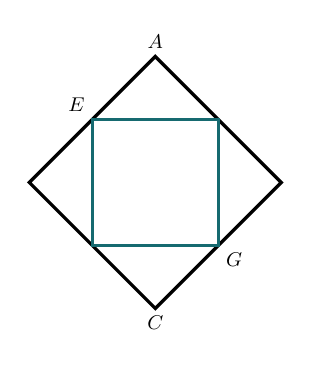
\begin{tikzpicture}[scale=.8,transform shape]
\draw[very thick] (0,2)--(-2,0)--(0,-2)--(2,0)--cycle;\draw[very thick,color=accent] (-1,1)--(-1,-1)--(1,-1)--(1,1)--cycle;\node[above] at (0,2) {$A$};\node[below] at (0,-2) {$C$};\node[above left] at (-1,1) {$E$};\node[below right] at (1,-1) {$G$};
\end{tikzpicture}
\figcaption{变图电试3.2V7\quad 第一有限内接层的八个电连接中点与顶点}
\end{minipage}\end{center}

\Needspace{20\baselineskip}
\item 保持中点连接几何，但调整各层材料或粗细，使第$j$层每边电阻为$q^jR_0$，$q>0$。求无限网络的两端口电阻。
\textbf{解：}变图电试3.2V8中第一层折叠半边为$b=qa$，$a=R_0/4$，隔两层的端口电阻为$q^2X$。令 $d=2ab/(a+b)$。对有限层截断，把每增加两层所对应的输入改写为 $F(X)=2a+d(2b+q^2X)/(d+2b+q^2X)$。$F$ 将非负终端映入 $[2a,2a+d]$，且
\[
0<F'(X)=\frac{d^2q^2}{(d+2b+q^2X)^2}
\le\left(\frac{q}{q+2}\right)^2<1.
\]
两种终端的输入差每加两层至多乘这个系数，故有限截断收敛到同一个固定值 $X=F(X)$。令$x=X/R_0$化简为$2qx^2+2(1-q)x-1=0$，正根$x=[q-1+\sqrt{q^2+1}]/(2q)$。$EG$的内侧网络电阻为$qX$，与外圈等效$R_0$并联，故$R_{EG}/R_0=qx/(1+qx)$。取$q=1/\sqrt2$恢复同材料、同粗细的两结果。
\begin{center}\begin{minipage}{.98\linewidth}\centering
\begin{tikzpicture}[scale=.8,transform shape]
\draw[axis] (0,0)--(10.7,0) node[right] {$q$};
\draw[axis] (0,0)--(0,3.2) node[above] {$R/R_0$};\foreach \y/\lab in {0/0,1.4/0.4,2.8/0.8}{\draw[thin] (0,\y)--(-.08,\y) node[left] {$\lab$};}
\node[above] at (5,3.5) {实线$AC$、虚线$EG$随逐层线阻缩放变化};
\draw[traj] plot coordinates {(0.500000000,1.837282337) (0.579166667,1.851016452) (0.658333333,1.864713299) (0.737500000,1.878368055) (0.816666667,1.891975998) (0.895833333,1.905532517) (0.975000000,1.919033121) (1.054166667,1.932473445) (1.133333333,1.945849265) (1.212500000,1.959156497) (1.291666667,1.972391206) (1.370833333,1.985549616) (1.450000000,1.998628108) (1.529166667,2.011623228) (1.608333333,2.024531688) (1.687500000,2.037350370) (1.766666667,2.050076328) (1.845833333,2.062706788) (1.925000000,2.075239145) (2.004166667,2.087670969) (2.083333333,2.100000000) (2.162500000,2.112224146) (2.241666667,2.124341483) (2.320833333,2.136350250) (2.400000000,2.148248849) (2.479166667,2.160035837) (2.558333333,2.171709927) (2.637500000,2.183269981) (2.716666667,2.194715006) (2.795833333,2.206044149) (2.875000000,2.217256694) (2.954166667,2.228352055) (3.033333333,2.239329772) (3.112500000,2.250189503) (3.191666667,2.260931026) (3.270833333,2.271554223) (3.350000000,2.282059085) (3.429166667,2.292445700) (3.508333333,2.302714252) (3.587500000,2.312865011) (3.666666667,2.322898333) (3.745833333,2.332814653) (3.825000000,2.342614480) (3.904166667,2.352298390) (3.983333333,2.361867028) (4.062500000,2.371321094) (4.141666667,2.380661349) (4.220833333,2.389888602) (4.300000000,2.399003713) (4.379166667,2.408007583) (4.458333333,2.416901155) (4.537500000,2.425685408) (4.616666667,2.434361354) (4.695833333,2.442930037) (4.775000000,2.451392526) (4.854166667,2.459749915) (4.933333333,2.468003319) (5.012500000,2.476153873) (5.091666667,2.484202726) (5.170833333,2.492151043) (5.250000000,2.500000000) (5.329166667,2.507750783) (5.408333333,2.515404585) (5.487500000,2.522962606) (5.566666667,2.530426049) (5.645833333,2.537796120) (5.725000000,2.545074028) (5.804166667,2.552260979) (5.883333333,2.559358178) (5.962500000,2.566366829) (6.041666667,2.573288131) (6.120833333,2.580123277) (6.200000000,2.586873456) (6.279166667,2.593539849) (6.358333333,2.600123631) (6.437500000,2.606625968) (6.516666667,2.613048015) (6.595833333,2.619390922) (6.675000000,2.625655824) (6.754166667,2.631843848) (6.833333333,2.637956111) (6.912500000,2.643993717) (6.991666667,2.649957758) (7.070833333,2.655849315) (7.150000000,2.661669455) (7.229166667,2.667419234) (7.308333333,2.673099695) (7.387500000,2.678711866) (7.466666667,2.684256766) (7.545833333,2.689735396) (7.625000000,2.695148747) (7.704166667,2.700497795) (7.783333333,2.705783502) (7.862500000,2.711006819) (7.941666667,2.716168681) (8.020833333,2.721270010) (8.100000000,2.726311715) (8.179166667,2.731294692) (8.258333333,2.736219823) (8.337500000,2.741087975) (8.416666667,2.745900005) (8.495833333,2.750656755) (8.575000000,2.755359054) (8.654166667,2.760007718) (8.733333333,2.764603551) (8.812500000,2.769147342) (8.891666667,2.773639871) (8.970833333,2.778081902) (9.050000000,2.782474189) (9.129166667,2.786817472) (9.208333333,2.791112480) (9.287500000,2.795359931) (9.366666667,2.799560529) (9.445833333,2.803714968) (9.525000000,2.807823930) (9.604166667,2.811888086) (9.683333333,2.815908096) (9.762500000,2.819884607) (9.841666667,2.823818259) (9.920833333,2.827709678) (10.000000000,2.831559480)};
\draw[dashed,thick,color=warm] plot coordinates {(0.500000000,0.174564674) (0.579166667,0.202032904) (0.658333333,0.229426598) (0.737500000,0.256736110) (0.816666667,0.283951996) (0.895833333,0.311065034) (0.975000000,0.338066241) (1.054166667,0.364946891) (1.133333333,0.391698530) (1.212500000,0.418312993) (1.291666667,0.444782413) (1.370833333,0.471099233) (1.450000000,0.497256216) (1.529166667,0.523246455) (1.608333333,0.549063375) (1.687500000,0.574700740) (1.766666667,0.600152657) (1.845833333,0.625413575) (1.925000000,0.650478290) (2.004166667,0.675341938) (2.083333333,0.700000000) (2.162500000,0.724448292) (2.241666667,0.748682966) (2.320833333,0.772700500) (2.400000000,0.796497697) (2.479166667,0.820071674) (2.558333333,0.843419854) (2.637500000,0.866539962) (2.716666667,0.889430011) (2.795833333,0.912088298) (2.875000000,0.934513388) (2.954166667,0.956704110) (3.033333333,0.978659543) (3.112500000,1.000379007) (3.191666667,1.021862051) (3.270833333,1.043108446) (3.350000000,1.064118170) (3.429166667,1.084891401) (3.508333333,1.105428503) (3.587500000,1.125730022) (3.666666667,1.145796667) (3.745833333,1.165629307) (3.825000000,1.185228960) (3.904166667,1.204596781) (3.983333333,1.223734055) (4.062500000,1.242642188) (4.141666667,1.261322698) (4.220833333,1.279777205) (4.300000000,1.298007426) (4.379166667,1.316015166) (4.458333333,1.333802309) (4.537500000,1.351370815) (4.616666667,1.368722708) (4.695833333,1.385860074) (4.775000000,1.402785052) (4.854166667,1.419499830) (4.933333333,1.436006638) (5.012500000,1.452307745) (5.091666667,1.468405452) (5.170833333,1.484302086) (5.250000000,1.500000000) (5.329166667,1.515501566) (5.408333333,1.530809170) (5.487500000,1.545925211) (5.566666667,1.560852097) (5.645833333,1.575592240) (5.725000000,1.590148056) (5.804166667,1.604521957) (5.883333333,1.618716356) (5.962500000,1.632733658) (6.041666667,1.646576261) (6.120833333,1.660246554) (6.200000000,1.673746912) (6.279166667,1.687079699) (6.358333333,1.700247263) (6.437500000,1.713251936) (6.516666667,1.726096031) (6.595833333,1.738781843) (6.675000000,1.751311647) (6.754166667,1.763687697) (6.833333333,1.775912223) (6.912500000,1.787987434) (6.991666667,1.799915516) (7.070833333,1.811698629) (7.150000000,1.823338909) (7.229166667,1.834838468) (7.308333333,1.846199389) (7.387500000,1.857423733) (7.466666667,1.868513532) (7.545833333,1.879470793) (7.625000000,1.890297494) (7.704166667,1.900995590) (7.783333333,1.911567005) (7.862500000,1.922013638) (7.941666667,1.932337362) (8.020833333,1.942540020) (8.100000000,1.952623431) (8.179166667,1.962589384) (8.258333333,1.972439645) (8.337500000,1.982175950) (8.416666667,1.991800011) (8.495833333,2.001313511) (8.575000000,2.010718109) (8.654166667,2.020015437) (8.733333333,2.029207102) (8.812500000,2.038294685) (8.891666667,2.047279742) (8.970833333,2.056163804) (9.050000000,2.064948377) (9.129166667,2.073634943) (9.208333333,2.082224960) (9.287500000,2.090719862) (9.366666667,2.099121058) (9.445833333,2.107429936) (9.525000000,2.115647860) (9.604166667,2.123776172) (9.683333333,2.131816191) (9.762500000,2.139769214) (9.841666667,2.147636518) (9.920833333,2.155419355) (10.000000000,2.163118961)};
\node[below] at (0,-.12) {$0$极限};
\node[below] at (3.5355339059327373,-.12) {$1/\sqrt2$};
\node[below] at (10,-.12) {$2$};
\end{tikzpicture}
\figcaption{变图电试3.2V8\quad 实线$AC$、虚线$EG$随逐层线阻缩放变化}
\end{minipage}\end{center}
\end{enumerate}

\Needspace{13\baselineskip}

\pdfbookmark[2]{第 3 题 双频理想电源驱动的稳态电流}{q3}

\section*{第 3 题\quad 双频理想电源驱动的稳态电流}\label{q:3}


两母线为$a,b$。理想电源$\mathcal E_1(t)=\mathcal E_0\sin^2\omega t$直接接于两母线，正方向使$V_a-V_b=\mathcal E_1$。上支路为电阻$R_2$与理想电源$\mathcal E_2(t)=\mathcal E_0\cos\omega t$串联，后者也以朝$a$方向升压为正。
中支路从$a$依次经过电感$L$，再通过并联的电容$C$和电阻$R_1$到$b$。已知
\[
R_1=R_2=R,\qquad L=\frac R{2\omega},\qquad
C=\frac1{2\omega R},
\]
电路已达到稳态。取流过$R_1$由左向右的电流为$i_1$，求$i_1(t)$并绘出曲线。说明$\mathcal E_2$是否影响$i_1$，以及稳态条件的作用。


\begin{center}\begin{minipage}{.98\linewidth}\centering
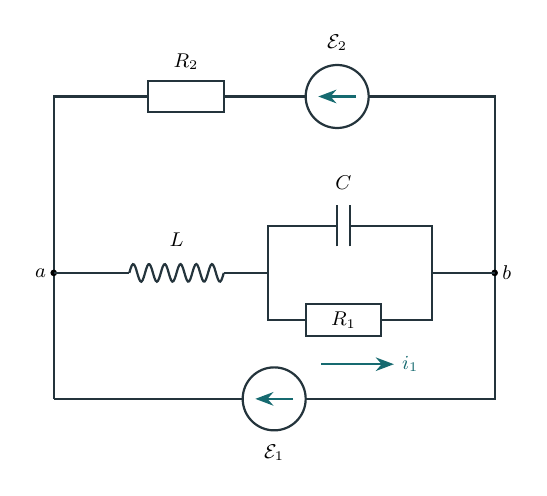
\begin{tikzpicture}[scale=.8,transform shape]

\draw[object] (0,-2)--(0,2.8)--(1.5,2.8);
\draw[object] (1.5,2.55) rectangle (2.7,3.05);
\draw[object] (2.7,2.8)--(4,2.8);
\draw[object] (4.5,2.8) circle (.5);
\draw[object] (5,2.8)--(7,2.8)--(7,-2)--(4,-2);
\draw[object] (3.5,-2) circle (.5);
\draw[object] (3,-2)--(0,-2);
\draw[motion] (3.8,-2)--(3.2,-2);
\draw[motion] (4.8,2.8)--(4.2,2.8);
\node[above] at (2.1,3.1) {$R_2$};
\node[above] at (4.5,3.4) {$\mathcal E_2$};
\node[below] at (3.5,-2.6) {$\mathcal E_1$};
\fill (0,0) circle (1.5pt) node[left] {$a$};
\fill (7,0) circle (1.5pt) node[right] {$b$};
\draw[object] (0,0)--(1.2,0);
\draw[object,domain=0:1.5,samples=80] plot ({1.2+\x},{.14*sin(1440*\x)});
\draw[object] (2.7,0)--(3.4,0)--(3.4,.75)--(4.5,.75);
\draw[object] (4.5,.42)--(4.5,1.08);\draw[object] (4.7,.42)--(4.7,1.08);
\draw[object] (4.7,.75)--(6,.75)--(6,-.75)--(5.2,-.75);
\draw[object] (4,-1) rectangle (5.2,-.5);
\draw[object] (4,-.75)--(3.4,-.75)--(3.4,0);
\draw[object] (6,0)--(7,0);
\node[above] at (1.95,.3) {$L$};
\node[above] at (4.6,1.2) {$C$};
\node at (4.6,-.75) {$R_1$};
\draw[motion] (4.25,-1.45)--(5.4,-1.45) node[right] {$i_1$};

\end{tikzpicture}
\figcaption{图电试3.3\quad 电源1直接固定母线电压，中支路为L串联电阻、电容的并联部分。}
\end{minipage}\end{center}

\Needspace{8\baselineskip}

\pdfbookmark[3]{题型定位}{q3-h0}

\subsection*{题型定位}

理想电压源直接跨接母线的多频稳态电路。先由连接关系确定中支路的输入，再把直流、二倍频分开计算。相量法按每个交流频率建立，输出在时域相加后形成有直流偏置的周期曲线；题设的稳态条件则选去初始储能的自由响应。

\Needspace{8\baselineskip}

\pdfbookmark[3]{知识点}{q3-h1}

\subsection*{知识点}

理想电压源规定自身端电压，电源叠加时置零对应短接。并联电阻和电容共用电压，电感电流为两支路电流之和；基尔霍夫定律给出二阶时域方程。直流稳态中电感压降为零、电容电流为零。各单频分量用同一复数约定表达，输入的负号也属于相位。偏置正弦的周期、极值与平均功率分别由频率、直流项和均方值决定。电阻使自由振荡的储能逐渐耗散。

\Needspace{8\baselineskip}

\pdfbookmark[3]{物理图像}{q3-h2}

\subsection*{物理图像}

题图$a,b$母线直接接电源1，电源2所在的上支路与中支路并列。解图电试3.3A把中支路的串联电感、并联$R_1,C$和共同电压$u$单独标出，图D的相量三角形说明两电流相差四分之一周期，电感电压再比总电流超前四分之一周期。图B画稳态电流的平均线、零点和极值，图C在相同输入下比较零储能接通的全过程与稳态，暂态差值逐渐衰减。

\Needspace{8\baselineskip}

\pdfbookmark[3]{解题入口}{q3-h3}

\subsection*{解题入口}

先问谁规定$V_a-V_b$，把$i_L=u/R+C\dot u$和电感压降写在图A旁。电源2通过上支路改变电源1承担的电流，中支路的输入已经给定。展开$\sin^2\omega t$后，直流用恒定响应，交流用$2\omega$的阻抗；最后以$t=0$处的值与斜率确定曲线从平均线向下出发。

\Needspace{8\baselineskip}

\pdfbookmark[3]{标准解法}{q3-h4}

\subsection*{标准解法}


图电试3.3中理想电源$\mathcal E_1$直接规定两母线电压$V_a-V_b=\mathcal E_1$。令电阻、电容共同的端电压为$u$，其左端相对$b$为正，电感电流$i_L$取向右。并联结点的流入电流等于电阻电流与充电电流之和，电感压降再与$u$相加：
\[
i_L=\frac uR+C\dot u,\qquad
L\dot i_L+u=\mathcal E_1.
\]
消去$i_L$，得到中支路的时域方程
\[
\boxed{LC\ddot u+\frac LR\dot u+u=\mathcal E_1(t)}.
\]
上支路电源2改变电源1承担的电流；中支路的输入始终是已给定的母线电压。上支路从$a$到$b$的电流为$(\mathcal E_1-\mathcal E_2)/R_2$，电源1随之补足两支路所需电流；这一连接关系先于任何频率计算成立。

把母线输入分解为
\[
\mathcal E_1=\frac{\mathcal E_0}{2}
-\frac{\mathcal E_0}{2}\cos2\omega t.
\]
直流稳态中$\dot i_L=0$、$\dot u=0$，电感压降为零、电容无电流，相当于电感短路、电容断路，故
\[
u_{\rm dc}=\frac{\mathcal E_0}{2},\qquad
i_{1,\rm dc}=\frac{\mathcal E_0}{2R}.
\]
这一恒定电压构成最后曲线的平均基线。剩下的交流项单独在角频率$2\omega$下计算。
\begin{center}\begin{minipage}{.98\linewidth}\centering
\begin{tikzpicture}[scale=.75,transform shape]

\draw[object] (0,-.5) circle (.45);
\draw[motion] (0,-.75)--(0,-.25);
\node[left] at (-.6,-.5) {$\widetilde{\mathcal E}$};
\draw[object] (0,-.05)--(0,1)--(1.3,1);
\draw[object] (1.3,.75) rectangle (3.1,1.25);
\node[above] at (2.2,1.4) {$j\Omega L$};
\draw[object] (3.1,1)--(5,1)--(5,.2);
\draw[object] (4.7,-1.2) rectangle (5.3,.2);
\node at (5,-.5) {$Z_p$};
\draw[object] (5,-1.2)--(5,-2)--(0,-2)--(0,-.95);
\draw[axis,<->] (6,-1.7)--(6,.7) node[midway,right] {$\widetilde u$};
\node at (2.8,-3) {$Z_p=R/(1+j\Omega RC),\quad H(2\omega)=-j$};
\node at (2.8,2.4) {$2\omega$交流等效；直流分量另算};

\end{tikzpicture}
\figcaption{解图电试3.3A\quad 并联端电压是输出量，负余弦输入与传函相位同时计入。}
\end{minipage}\end{center}
对角频率$\Omega$的余弦分量采用$e^{j\Omega t}$约定。解图电试3.3A中的并联阻抗由电导相加给出，输出$\widetilde u$是该阻抗的端电压，因此
\[
Z_p=\frac{R}{1+j\Omega RC},\qquad
H(\Omega)=\frac{\widetilde u}{\widetilde{\mathcal E}}
=\frac{Z_p}{j\Omega L+Z_p}
=\frac1{1-\Omega^2LC+j\Omega L/R}.
\]
分母实部来自电感、电容的共同作用，虚部来自电阻电流对应的电感压降。题设$\Omega=2\omega$时，$2\omega L=R$、$1/(2\omega C)=R$，即电感电抗、电容电抗和电阻数值相等。
\begin{center}\begin{minipage}{.98\linewidth}\centering
\begin{tikzpicture}[scale=.8,transform shape]
\draw[axis] (0,0)--(4.3,0) node[right] {$\widetilde U_{RC}$};\draw[motion] (0,0)--(0,2) node[above left] {$\widetilde I_C$};\draw[motion] (0,0)--(2,0) node[below] {$\widetilde I_R$};\draw[motion] (0,0)--(2,2) node[above right] {$\widetilde I$};\draw[guide] (0,2)--(2,2)--(2,0);\draw[force] (0,0)--(-4,4) node[left] {$\widetilde U_L$};\draw[force] (0,0)--(0,4) node[above right] {$\widetilde U$};\draw[guide] (-4,4)--(0,4)--(4,0);\draw (0.7,0) arc(0:45:.7);\node at (1,.4) {$45^\circ$};\node[align=center] at (0,-1.2) {以正余弦辅助输入定向；电流与电压分别使用比例尺};
\end{tikzpicture}
\figcaption{解图电试3.3D\quad 并联相量与串联电压相加，实际负余弦分量再计入负号}
\end{minipage}\end{center}
解图电试3.3D先用正余弦辅助激励定相位，取$\widetilde U_{RC}$水平向右。电阻电流同向，电容电流超前$90^\circ$且幅值相等，所以$I=\sqrt2 I_R$、总电流沿$45^\circ$。电感电压再超前总电流$90^\circ$，其幅值$U_L=I(2\omega)L=\sqrt2 U_{RC}$，分量为$(-U_{RC},U_{RC})$。与并联电压$(U_{RC},0)$相加，输入电压恰沿竖直向上，幅值仍为$U_{RC}$；并联电压落后输入$90^\circ$。同一关系写成复数，就是$\Omega^2LC=1$、$\Omega L/R=1$时
\[
H(2\omega)=\frac1j=-j.
\]
实际交流输入为负余弦，复振幅是$-\mathcal E_0/2$。把它与上述传递系数相乘再取实部，
\[
\widetilde u_{\rm ac}
=(-j)\left(-\frac{\mathcal E_0}{2}\right)
=j\frac{\mathcal E_0}{2},\qquad
u_{\rm ac}=\Re\left[j\frac{\mathcal E_0}{2}e^{j2\omega t}\right]
=-\frac{\mathcal E_0}{2}\sin2\omega t.
\]
负余弦的复振幅为负实数，与传递相位一起决定输出的正负。正余弦辅助电路中$i_R=\mathcal E_0\sin2\omega t/(2R)$，实际分量则为$-i_R$；这与复振幅的乘法是同一步相位关系的两种表示。再叠加直流，得到
\[
\boxed{i_1(t)=\frac{\mathcal E_0}{2R}
\bigl(1-\sin2\omega t\bigr)}.
\]
\begin{center}\begin{minipage}{.98\linewidth}\centering
\begin{tikzpicture}[scale=.8,transform shape]
\draw[axis] (0,0)--(10.7,0) node[right] {$\omega t$};
\draw[axis] (0,0)--(0,3.2) node[above] {$i_1R/\mathcal E_0$};\foreach \y/\lab in {0/0,1.5/0.5,3/1}{\draw[thin] (0,\y)--(-.08,\y) node[left] {$\lab$};}
\node[above] at (5,3.5) {周期$\pi/\omega$，平均值$1/2$，先从平均线向下};
\draw[traj] plot coordinates {(0.000000000,1.500000000) (0.062500000,1.382311356) (0.125000000,1.265348302) (0.187500000,1.149831954) (0.250000000,1.036474508) (0.312500000,0.925974851) (0.375000000,0.819014250) (0.437500000,0.716252153) (0.500000000,0.618322122) (0.562500000,0.525827928) (0.625000000,0.439339828) (0.687500000,0.359391052) (0.750000000,0.286474508) (0.812500000,0.221039753) (0.875000000,0.163490214) (0.937500000,0.114180701) (1.000000000,0.073415226) (1.062500000,0.041445119) (1.125000000,0.018467489) (1.187500000,0.004623999) (1.250000000,0.000000000) (1.312500000,0.004623999) (1.375000000,0.018467489) (1.437500000,0.041445119) (1.500000000,0.073415226) (1.562500000,0.114180701) (1.625000000,0.163490214) (1.687500000,0.221039753) (1.750000000,0.286474508) (1.812500000,0.359391052) (1.875000000,0.439339828) (1.937500000,0.525827928) (2.000000000,0.618322122) (2.062500000,0.716252153) (2.125000000,0.819014250) (2.187500000,0.925974851) (2.250000000,1.036474508) (2.312500000,1.149831954) (2.375000000,1.265348302) (2.437500000,1.382311356) (2.500000000,1.500000000) (2.562500000,1.617688644) (2.625000000,1.734651698) (2.687500000,1.850168046) (2.750000000,1.963525492) (2.812500000,2.074025149) (2.875000000,2.180985750) (2.937500000,2.283747847) (3.000000000,2.381677878) (3.062500000,2.474172072) (3.125000000,2.560660172) (3.187500000,2.640608948) (3.250000000,2.713525492) (3.312500000,2.778960247) (3.375000000,2.836509786) (3.437500000,2.885819299) (3.500000000,2.926584774) (3.562500000,2.958554881) (3.625000000,2.981532511) (3.687500000,2.995376001) (3.750000000,3.000000000) (3.812500000,2.995376001) (3.875000000,2.981532511) (3.937500000,2.958554881) (4.000000000,2.926584774) (4.062500000,2.885819299) (4.125000000,2.836509786) (4.187500000,2.778960247) (4.250000000,2.713525492) (4.312500000,2.640608948) (4.375000000,2.560660172) (4.437500000,2.474172072) (4.500000000,2.381677878) (4.562500000,2.283747847) (4.625000000,2.180985750) (4.687500000,2.074025149) (4.750000000,1.963525492) (4.812500000,1.850168046) (4.875000000,1.734651698) (4.937500000,1.617688644) (5.000000000,1.500000000) (5.062500000,1.382311356) (5.125000000,1.265348302) (5.187500000,1.149831954) (5.250000000,1.036474508) (5.312500000,0.925974851) (5.375000000,0.819014250) (5.437500000,0.716252153) (5.500000000,0.618322122) (5.562500000,0.525827928) (5.625000000,0.439339828) (5.687500000,0.359391052) (5.750000000,0.286474508) (5.812500000,0.221039753) (5.875000000,0.163490214) (5.937500000,0.114180701) (6.000000000,0.073415226) (6.062500000,0.041445119) (6.125000000,0.018467489) (6.187500000,0.004623999) (6.250000000,0.000000000) (6.312500000,0.004623999) (6.375000000,0.018467489) (6.437500000,0.041445119) (6.500000000,0.073415226) (6.562500000,0.114180701) (6.625000000,0.163490214) (6.687500000,0.221039753) (6.750000000,0.286474508) (6.812500000,0.359391052) (6.875000000,0.439339828) (6.937500000,0.525827928) (7.000000000,0.618322122) (7.062500000,0.716252153) (7.125000000,0.819014250) (7.187500000,0.925974851) (7.250000000,1.036474508) (7.312500000,1.149831954) (7.375000000,1.265348302) (7.437500000,1.382311356) (7.500000000,1.500000000) (7.562500000,1.617688644) (7.625000000,1.734651698) (7.687500000,1.850168046) (7.750000000,1.963525492) (7.812500000,2.074025149) (7.875000000,2.180985750) (7.937500000,2.283747847) (8.000000000,2.381677878) (8.062500000,2.474172072) (8.125000000,2.560660172) (8.187500000,2.640608948) (8.250000000,2.713525492) (8.312500000,2.778960247) (8.375000000,2.836509786) (8.437500000,2.885819299) (8.500000000,2.926584774) (8.562500000,2.958554881) (8.625000000,2.981532511) (8.687500000,2.995376001) (8.750000000,3.000000000) (8.812500000,2.995376001) (8.875000000,2.981532511) (8.937500000,2.958554881) (9.000000000,2.926584774) (9.062500000,2.885819299) (9.125000000,2.836509786) (9.187500000,2.778960247) (9.250000000,2.713525492) (9.312500000,2.640608948) (9.375000000,2.560660172) (9.437500000,2.474172072) (9.500000000,2.381677878) (9.562500000,2.283747847) (9.625000000,2.180985750) (9.687500000,2.074025149) (9.750000000,1.963525492) (9.812500000,1.850168046) (9.875000000,1.734651698) (9.937500000,1.617688644) (10.000000000,1.500000000)};
\node[below] at (1.25,-.12) {$\pi/4$};
\node[below] at (3.75,-.12) {$3\pi/4$};
\node[below] at (6.25,-.12) {$5\pi/4$};
\node[below] at (8.75,-.12) {$7\pi/4$};
\end{tikzpicture}
\figcaption{解图电试3.3B\quad 周期$\pi/\omega$，平均值$1/2$，先从平均线向下}
\end{minipage}\end{center}
解图电试3.3B以$\omega t$为横坐标，电流用$\mathcal E_0/R$归一化。因为$\sin2\omega t$每经过$\pi/\omega$重复一次，电流周期为$\pi/\omega$，平均值为$\mathcal E_0/(2R)$，全程非负。极值为
\[
i_{1,\min}=0\quad
(\omega t=\pi/4+k\pi),\qquad
i_{1,\max}=\frac{\mathcal E_0}{R}\quad
(\omega t=3\pi/4+k\pi).
\]
在$t=0$，$i_1=\mathcal E_0/(2R)$且$\dot i_1=-\mathcal E_0\omega/R$；到$\omega t=\pi/4$降到零，再在$\pi/2$回到平均线向上，通过$3\pi/4$的最高点。曲线在平均线起步，先向下到达零点。

按电源叠加单独计算$\mathcal E_2$时，理想电源1置零成为连接$a,b$的导线。中支路的外加电压随之为零，周期稳态响应为零，故电源2对$i_1$的稳态贡献为$i(3)=0$。电源2仍可向上支路供能，其电流由电源1的短接支路回流。

稳态条件决定怎样处理初始储能。将给定参数代入齐次方程，
\[
\ddot u+2\omega\dot u+4\omega^2u=0,
\]
特征方程$s^2+2\omega s+4\omega^2=0$的根为$-\omega\pm j\sqrt3\,\omega$，所以一般响应在周期部分外还有
\[
u_h=e^{-\omega t}
\left(A\cos\sqrt3\,\omega t+B\sin\sqrt3\,\omega t\right).
\]
\begin{center}\begin{minipage}{.98\linewidth}\centering
\begin{tikzpicture}[scale=.8,transform shape]
\draw[axis] (0,0)--(10.7,0) node[right] {$\omega t$};
\draw[axis] (0,0)--(0,3.2) node[above] {$i_1R/\mathcal E_0$};\foreach \y/\lab in {0/0,1.4/0.5,2.8/1}{\draw[thin] (0,\y)--(-.08,\y) node[left] {$\lab$};}
\node[above] at (5,3.5) {实线：零储能接通；虚线：周期稳态};
\draw[traj] plot coordinates {(0.000000000,0.000000000) (0.071428571,0.000005715) (0.142857143,0.000089483) (0.214285714,0.000442854) (0.285714286,0.001366810) (0.357142857,0.003255194) (0.428571429,0.006577557) (0.500000000,0.011861707) (0.571428571,0.019676193) (0.642857143,0.030612968) (0.714285714,0.045270480) (0.785714286,0.064237366) (0.857142857,0.088076986) (0.928571429,0.117312938) (1.000000000,0.152415734) (1.071428571,0.193790771) (1.142857143,0.241767707) (1.214285714,0.296591346) (1.285714286,0.358414104) (1.357142857,0.427290109) (1.428571429,0.503170973) (1.500000000,0.585903239) (1.571428571,0.675227503) (1.642857143,0.770779182) (1.714285714,0.872090876) (1.785714286,0.978596268) (1.857142857,1.089635481) (1.928571429,1.204461788) (2.000000000,1.322249582) (2.071428571,1.442103469) (2.142857143,1.563068365) (2.214285714,1.684140448) (2.285714286,1.804278824) (2.357142857,1.922417745) (2.428571429,2.037479232) (2.500000000,2.148385938) (2.571428571,2.254074090) (2.642857143,2.353506353) (2.714285714,2.445684467) (2.785714286,2.529661493) (2.857142857,2.604553538) (2.928571429,2.669550806) (3.000000000,2.723927866) (3.071428571,2.767053002) (3.142857143,2.798396541) (3.214285714,2.817538079) (3.285714286,2.824172500) (3.357142857,2.818114741) (3.428571429,2.799303235) (3.500000000,2.767802008) (3.571428571,2.723801389) (3.642857143,2.667617337) (3.714285714,2.599689393) (3.785714286,2.520577267) (3.857142857,2.430956112) (3.928571429,2.331610520) (4.000000000,2.223427314) (4.071428571,2.107387214) (4.142857143,1.984555456) (4.214285714,1.856071474) (4.285714286,1.723137744) (4.357142857,1.587007921) (4.428571429,1.448974382) (4.500000000,1.310355308) (4.571428571,1.172481454) (4.642857143,1.036682723) (4.714285714,0.904274706) (4.785714286,0.776545320) (4.857142857,0.654741681) (4.928571429,0.540057353) (5.000000000,0.433620109) (5.071428571,0.336480326) (5.142857143,0.249600139) (5.214285714,0.173843461) (5.285714286,0.109966989) (5.357142857,0.058612266) (5.428571429,0.020298906) (5.500000000,-0.004580964) (5.571428571,-0.015766981) (5.642857143,-0.013133490) (5.714285714,0.003308866) (5.785714286,0.033412932) (5.857142857,0.076896212) (5.928571429,0.133343405) (6.000000000,0.202210290) (6.071428571,0.282828918) (6.142857143,0.374414058) (6.214285714,0.476070837) (6.285714286,0.586803497) (6.357142857,0.705525177) (6.428571429,0.831068629) (6.500000000,0.962197750) (6.571428571,1.097619829) (6.642857143,1.235998370) (6.714285714,1.375966374) (6.785714286,1.516139941) (6.857142857,1.655132055) (6.928571429,1.791566415) (7.000000000,1.924091171) (7.071428571,2.051392431) (7.142857143,2.172207392) (7.214285714,2.285336980) (7.285714286,2.389657855) (7.357142857,2.484133668) (7.428571429,2.567825459) (7.500000000,2.639901080) (7.571428571,2.699643563) (7.642857143,2.746458339) (7.714285714,2.779879232) (7.785714286,2.799573177) (7.857142857,2.805343607) (7.928571429,2.797132482) (8.000000000,2.775020922) (8.071428571,2.739228461) (8.142857143,2.690110912) (8.214285714,2.628156865) (8.285714286,2.553982867) (8.357142857,2.468327306) (8.428571429,2.372043090) (8.500000000,2.266089169) (8.571428571,2.151520996) (8.642857143,2.029480029) (8.714285714,1.901182355) (8.785714286,1.767906580) (8.857142857,1.630981083) (8.928571429,1.491770772) (9.000000000,1.351663467) (9.071428571,1.212056059) (9.142857143,1.074340572) (9.214285714,0.939890266) (9.285714286,0.810045931) (9.357142857,0.686102499) (9.428571429,0.569296114) (9.500000000,0.460791786) (9.571428571,0.361671752) (9.642857143,0.272924667) (9.714285714,0.195435721) (9.785714286,0.129977794) (9.857142857,0.077203729) (9.928571429,0.037639806) (10.000000000,0.011680474)};
\draw[dashed,thick,color=warm] plot coordinates {(0.000000000,1.400000000) (0.071428571,1.260233217) (0.142857143,1.121862937) (0.214285714,0.986271711) (0.285714286,0.854814321) (0.357142857,0.728804246) (0.428571429,0.609500537) (0.500000000,0.498095238) (0.571428571,0.395701473) (0.642857143,0.303342327) (0.714285714,0.221940621) (0.785714286,0.152309696) (0.857142857,0.095145280) (0.928571429,0.051018540) (1.000000000,0.020370378) (1.071428571,0.003507019) (1.142857143,0.000596956) (1.214285714,0.011669265) (1.285714286,0.036613317) (1.357142857,0.075179877) (1.428571429,0.126983602) (1.500000000,0.191506887) (1.571428571,0.268105035) (1.642857143,0.356012703) (1.714285714,0.454351547) (1.785714286,0.562138998) (1.857142857,0.678298079) (1.928571429,0.801668168) (2.000000000,0.931016590) (2.071428571,1.065050939) (2.142857143,1.202431989) (2.214285714,1.341787073) (2.285714286,1.481723801) (2.357142857,1.620843972) (2.428571429,1.757757543) (2.500000000,1.891096519) (2.571428571,2.019528621) (2.642857143,2.141770597) (2.714285714,2.256601047) (2.785714286,2.362872623) (2.857142857,2.459523493) (2.928571429,2.545587955) (3.000000000,2.620206081) (3.071428571,2.682632311) (3.142857143,2.732242903) (3.214285714,2.768542165) (3.285714286,2.791167405) (3.357142857,2.799892561) (3.428571429,2.794630452) (3.500000000,2.775433658) (3.571428571,2.742493985) (3.642857143,2.696140555) (3.714285714,2.636836518) (3.785714286,2.565174419) (3.857142857,2.481870283) (3.928571429,2.387756456) (4.000000000,2.283773293) (4.071428571,2.170959760) (4.142857143,2.050443051) (4.214285714,1.923427331) (4.285714286,1.791181697) (4.357142857,1.655027506) (4.428571429,1.516325164) (4.500000000,1.376460539) (4.571428571,1.236831113) (4.642857143,1.098832017) (4.714285714,0.963842091) (4.785714286,0.833210111) (4.857142857,0.708241308) (4.928571429,0.590184330) (5.000000000,0.480218762) (5.071428571,0.379443344) (5.142857143,0.288864991) (5.214285714,0.209388731) (5.285714286,0.141808666) (5.357142857,0.086800033) (5.428571429,0.044912459) (5.500000000,0.016564473) (5.571428571,0.002039316) (5.642857143,0.001482121) (5.714285714,0.014898455) (5.785714286,0.042154265) (5.857142857,0.082977221) (5.928571429,0.136959433) (6.000000000,0.203561529) (6.071428571,0.282118042) (6.142857143,0.371844063) (6.214285714,0.471843078) (6.285714286,0.581115930) (6.357142857,0.698570801) (6.428571429,0.823034121) (6.500000000,0.953262293) (6.571428571,1.087954120) (6.642857143,1.225763807) (6.714285714,1.365314404) (6.785714286,1.505211569) (6.857142857,1.644057494) (6.928571429,1.780464877) (7.000000000,1.913070781) (7.071428571,2.040550251) (7.142857143,2.161629555) (7.214285714,2.275098908) (7.285714286,2.379824563) (7.357142857,2.474760134) (7.428571429,2.558957057) (7.500000000,2.631574064) (7.571428571,2.691885590) (7.642857143,2.739289023) (7.714285714,2.773310722) (7.785714286,2.793610755) (7.857142857,2.799986289) (7.928571429,2.792373623) (8.000000000,2.770848821) (8.071428571,2.735626950) (8.142857143,2.687059936) (8.214285714,2.625633045) (8.285714286,2.551960033) (8.357142857,2.466777017) (8.428571429,2.370935119) (8.500000000,2.265391957) (8.571428571,2.151202085) (8.642857143,2.029506450) (8.714285714,1.901520995) (8.785714286,1.768524508) (8.857142857,1.631845846) (8.928571429,1.492850656) (9.000000000,1.352927734) (9.071428571,1.213475142) (9.142857143,1.075886245) (9.214285714,0.941535785) (9.285714286,0.811766148) (9.357142857,0.687873950) (9.428571429,0.571097079) (9.500000000,0.462602333) (9.571428571,0.363473754) (9.642857143,0.274701803) (9.714285714,0.197173459) (9.785714286,0.131663361) (9.857142857,0.078826063) (9.928571429,0.039189498) (10.000000000,0.013149702)};
\node[below] at (0,-.12) {$0$};
\node[below] at (5,-.12) {$3.5$};
\node[below] at (10,-.12) {$7$};
\end{tikzpicture}
\figcaption{解图电试3.3C\quad 实线：零储能接通；虚线：周期稳态}
\end{minipage}\end{center}
解图电试3.3C取同一输入从$t=0$接通，电容电压和电感电流均从零开始作比较。此时$u(0)=0$，结点式给$\dot u(0)=0$，而周期解在零时刻分别为$\mathcal E_0/2$、$-\mathcal E_0\omega$；两者之差确定$A=-\mathcal E_0/2$、$B=\mathcal E_0/(2\sqrt3)$。指数因子使差值在时间尺度$1/\omega$上衰减。题设已达到稳定状态，保留的是图B的周期部分。理想电源规定端电压，初始储能形成图C中的衰减分量，其幅值由接通时的电压和电流确定。



\Needspace{8\baselineskip}

\pdfbookmark[3]{关键洞察}{q3-h5}

\subsection*{关键洞察}

理想电源控制的是母线电压，它同时承担各支路所需的电流。因此电源2虽不改变$i_1$，仍参与供能并改变电源1输出的电流。$2\omega$时传递函数为$-j$，给出有限幅值和四分之一周期的滞后；输入的负余弦随后决定实际输出的正负。任意初始电感电流和电容电压还给自由响应，经过电阻耗散后才得到题设的周期稳态。

\Needspace{8\baselineskip}

\pdfbookmark[3]{易错点}{q3-h6}

\subsection*{易错点}

输入$\sin^2\omega t$包含直流与$2\omega$，两部分分别计算。理想电压源置零后用导线替代，有限内阻电源则保留内阻。图A中电阻与电容共用$u$，电感电流由结点守恒相加；电阻耗散使$\Omega^2LC=1$时幅值保持有限。计算复振幅时同时保留输入负号和$H=-j$，作图使用周期$\pi/\omega$及起点$\mathcal E_0/(2R)$。发热由电流均方值给出，初始储能则单独进入自由响应。

\Needspace{8\baselineskip}

\pdfbookmark[3]{课堂讲解建议}{q3-h7}

\subsection*{课堂讲解建议}

先遮住电源2的数值，要求根据三支路的连接关系说出母线电压。让学生在图A结点写出两种电流，再由回路方程消去电感电流，这样能解释电源2为何未进入中支路方程。

处理交流时把图D中的$U_{RC}$取作参考，先由并联电压画两支路电流，再由总电流画电感电压。说明正余弦辅助激励的输出后，把实际输入的负号放回复振幅。画图前列$\omega t=0,\pi/4,\pi/2,3\pi/4$四点并写出斜率，随后连成图B。最后撤去稳态条件，让学生用电容电压和电感电流连续确定图C的两个暂态常数，把“电源规定端电压”和“电感、电容保存初始状态”联系起来。

\Needspace{8\baselineskip}

\pdfbookmark[3]{变式训练}{q3-h8}

\subsection*{变式训练}

\begin{enumerate}
\Needspace{20\baselineskip}
\item 中支路参数为任意正数$R,L,C$，输入单独改为$E_a\cos\Omega t$，求稳态电阻电流的幅值和相位。
\textbf{解：}变图电试3.3V1以并联端电压为输出。写$\widetilde i_L=(1/R+j\Omega C)\widetilde u$，再由$\widetilde E=j\Omega L\widetilde i_L+\widetilde u$得$\widetilde u=E_a/[1-\Omega^2LC+j\Omega L/R]$。所以电流振幅为$E_a/[R\sqrt{(1-\Omega^2LC)^2+(\Omega L/R)^2}]$，相位为$-\arg[1-\Omega^2LC+j\Omega L/R]$，用含象限的辐角描述整个频域。$\Omega\to0$时电流趋于$E_a/R$，高频时电容电压随$\Omega^{-2}$降低。
\begin{center}\begin{minipage}{.98\linewidth}\centering
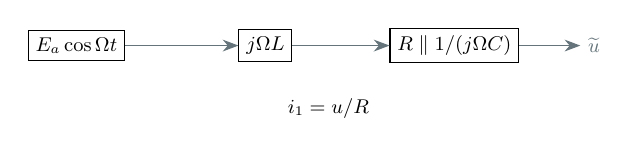
\begin{tikzpicture}[scale=.8,transform shape]
\node[draw] (in) at (0,0) {$E_a\cos\Omega t$};\node[draw] (l) at (3,0) {$j\Omega L$};\node[draw] (p) at (6,0) {$R\parallel 1/(j\Omega C)$};\draw[axis] (in)--(l);\draw[axis] (l)--(p);\draw[axis] (p)--(8,0) node[right] {$\widetilde u$};\node at (4,-1) {$i_1=u/R$};
\end{tikzpicture}
\figcaption{变图电试3.3V1\quad 任意单频激励下的同一电压传递关系}
\end{minipage}\end{center}

\Needspace{20\baselineskip}
\item 保持题设参数，把母线电压改为$\mathcal E_0\cos\omega t$，求电阻电流并与二倍频结果比较。
\textbf{解：}变图电试3.3V2此时$\Omega^2LC=1/4$、$\Omega L/R=1/2$。因此$H(\omega)=1/(3/4+j/2)=(12-8j)/13$，幅值为$4/\sqrt{13}$，相位滞后$\arctan(2/3)$。电流为$4\mathcal E_0/(R\sqrt{13})\cos[\omega t-\arctan(2/3)]$，也等于$\mathcal E_0(12\cos\omega t+8\sin\omega t)/(13R)$。电感和电容在一个周期内往返交换能量，电阻上的电压幅值可略大于输入幅值，供能仍由电源提供。
\begin{center}\begin{minipage}{.98\linewidth}\centering
\begin{tikzpicture}[scale=.8,transform shape]
\draw[axis] (0,0)--(10.7,0) node[right] {$\omega t$};
\draw[axis] (0,0)--(0,4) node[above] {$i_1R/\mathcal E_0$};\foreach \y/\lab in {0.3/-1,1.8/0,3.3/1}{\draw[thin] (0,\y)--(-.08,\y) node[left] {$\lab$};}
\node[above] at (5,4.5) {输入频率为$\omega$时的稳态电流};
\draw[traj] plot coordinates {(0.000000000,3.184615385) (0.083333333,3.231027931) (0.166666667,3.273518129) (0.250000000,3.311969516) (0.333333333,3.346276700) (0.416666667,3.376345647) (0.500000000,3.402093940) (0.583333333,3.423451005) (0.666666667,3.440358304) (0.750000000,3.452769495) (0.833333333,3.460650559) (0.916666667,3.463979896) (1.000000000,3.462748379) (1.083333333,3.456959385) (1.166666667,3.446628780) (1.250000000,3.431784880) (1.333333333,3.412468371) (1.416666667,3.388732198) (1.500000000,3.360641421) (1.583333333,3.328273034) (1.666666667,3.291715757) (1.750000000,3.251069791) (1.833333333,3.206446544) (1.916666667,3.157968324) (2.000000000,3.105768007) (2.083333333,3.049988671) (2.166666667,2.990783203) (2.250000000,2.928313881) (2.333333333,2.862751929) (2.416666667,2.794277048) (2.500000000,2.723076923) (2.583333333,2.649346708) (2.666666667,2.573288493) (2.750000000,2.495110747) (2.833333333,2.415027752) (2.916666667,2.333259008) (3.000000000,2.250028638) (3.083333333,2.165564771) (3.166666667,2.080098917) (3.250000000,1.993865330) (3.333333333,1.907100373) (3.416666667,1.820041860) (3.500000000,1.732928415) (3.583333333,1.645998808) (3.666666667,1.559491307) (3.750000000,1.473643024) (3.833333333,1.388689263) (3.916666667,1.304862876) (4.000000000,1.222393625) (4.083333333,1.141507554) (4.166666667,1.062426364) (4.250000000,0.985366812) (4.333333333,0.910540114) (4.416666667,0.838151363) (4.500000000,0.768398972) (4.583333333,0.701474128) (4.666666667,0.637560267) (4.750000000,0.576832573) (4.833333333,0.519457496) (4.916666667,0.465592296) (5.000000000,0.415384615) (5.083333333,0.368972069) (5.166666667,0.326481871) (5.250000000,0.288030484) (5.333333333,0.253723300) (5.416666667,0.223654353) (5.500000000,0.197906060) (5.583333333,0.176548995) (5.666666667,0.159641696) (5.750000000,0.147230505) (5.833333333,0.139349441) (5.916666667,0.136020104) (6.000000000,0.137251621) (6.083333333,0.143040615) (6.166666667,0.153371220) (6.250000000,0.168215120) (6.333333333,0.187531629) (6.416666667,0.211267802) (6.500000000,0.239358579) (6.583333333,0.271726966) (6.666666667,0.308284243) (6.750000000,0.348930209) (6.833333333,0.393553456) (6.916666667,0.442031676) (7.000000000,0.494231993) (7.083333333,0.550011329) (7.166666667,0.609216797) (7.250000000,0.671686119) (7.333333333,0.737248071) (7.416666667,0.805722952) (7.500000000,0.876923077) (7.583333333,0.950653292) (7.666666667,1.026711507) (7.750000000,1.104889253) (7.833333333,1.184972248) (7.916666667,1.266740992) (8.000000000,1.349971362) (8.083333333,1.434435229) (8.166666667,1.519901083) (8.250000000,1.606134670) (8.333333333,1.692899627) (8.416666667,1.779958140) (8.500000000,1.867071585) (8.583333333,1.954001192) (8.666666667,2.040508693) (8.750000000,2.126356976) (8.833333333,2.211310737) (8.916666667,2.295137124) (9.000000000,2.377606375) (9.083333333,2.458492446) (9.166666667,2.537573636) (9.250000000,2.614633188) (9.333333333,2.689459886) (9.416666667,2.761848637) (9.500000000,2.831601028) (9.583333333,2.898525872) (9.666666667,2.962439733) (9.750000000,3.023167427) (9.833333333,3.080542504) (9.916666667,3.134407704) (10.000000000,3.184615385)};
\node[below] at (0,-.12) {$0$};
\node[below] at (5,-.12) {$\pi$};
\node[below] at (10,-.12) {$2\pi$};
\end{tikzpicture}
\figcaption{变图电试3.3V2\quad 输入频率为$\omega$时的稳态电流}
\end{minipage}\end{center}

\Needspace{20\baselineskip}
\item 求题设稳态中$R_1$的平均功率，并说明平均电流和有效值的区别。
\textbf{解：}变图电试3.3V3把电流分成平均值$\mathcal E_0/(2R)$与零平均正弦。平方后交叉项的周期平均为零，而$\langle\sin^22\omega t\rangle=1/2$，故$\langle i_1^2\rangle=\mathcal E_0^2(1+1/2)/(4R^2)=3\mathcal E_0^2/(8R^2)$。于是$P_{R_1}=3\mathcal E_0^2/(8R)$，有效值为$\sqrt{3/8}\mathcal E_0/R$。平均电流平方只给直流发热$\mathcal E_0^2/(4R)$，交流分量另贡献$\mathcal E_0^2/(8R)$。
\begin{center}\begin{minipage}{.98\linewidth}\centering
\begin{tikzpicture}[scale=.8,transform shape]
\draw[axis] (0,0)--(10.7,0) node[right] {$\omega t$};
\draw[axis] (0,0)--(0,3.2) node[above] {$p_{R_1}R/\mathcal E_0^2$};\foreach \y/\lab in {0/0,1.5/0.5,3/1}{\draw[thin] (0,\y)--(-.08,\y) node[left] {$\lab$};}
\node[above] at (5,3.5) {瞬时功率的周期平均为$3/8$};
\draw[traj] plot coordinates {(0.000000000,0.750000000) (0.083333333,0.673550355) (0.166666667,0.601401955) (0.250000000,0.533702109) (0.333333333,0.470552917) (0.416666667,0.412011906) (0.500000000,0.358093136) (0.583333333,0.308768766) (0.666666667,0.263971058) (0.750000000,0.223594781) (0.833333333,0.187500000) (0.916666667,0.155515206) (1.000000000,0.127440749) (1.083333333,0.103052529) (1.166666667,0.082105917) (1.250000000,0.064339828) (1.333333333,0.049480936) (1.416666667,0.037247942) (1.500000000,0.027355881) (1.583333333,0.019520389) (1.666666667,0.013461894) (1.750000000,0.008909683) (1.833333333,0.005605791) (1.916666667,0.003308670) (2.000000000,0.001796598) (2.083333333,0.000870787) (2.166666667,0.000358146) (2.250000000,0.000113683) (2.333333333,0.000022507) (2.416666667,0.000001409) (2.500000000,0.000000000) (2.583333333,0.000001409) (2.666666667,0.000022507) (2.750000000,0.000113683) (2.833333333,0.000358146) (2.916666667,0.000870787) (3.000000000,0.001796598) (3.083333333,0.003308670) (3.166666667,0.005605791) (3.250000000,0.008909683) (3.333333333,0.013461894) (3.416666667,0.019520389) (3.500000000,0.027355881) (3.583333333,0.037247942) (3.666666667,0.049480936) (3.750000000,0.064339828) (3.833333333,0.082105917) (3.916666667,0.103052529) (4.000000000,0.127440749) (4.083333333,0.155515206) (4.166666667,0.187500000) (4.250000000,0.223594781) (4.333333333,0.263971058) (4.416666667,0.308768766) (4.500000000,0.358093136) (4.583333333,0.412011906) (4.666666667,0.470552917) (4.750000000,0.533702109) (4.833333333,0.601401955) (4.916666667,0.673550355) (5.000000000,0.750000000) (5.083333333,0.830558224) (5.166666667,0.914987345) (5.250000000,1.003005504) (5.333333333,1.094287990) (5.416666667,1.188469041) (5.500000000,1.285144119) (5.583333333,1.383872615) (5.666666667,1.484180987) (5.750000000,1.585566280) (5.833333333,1.687500000) (5.916666667,1.789432311) (6.000000000,1.890796506) (6.083333333,1.991013703) (6.166666667,2.089497736) (6.250000000,2.185660172) (6.333333333,2.278915412) (6.416666667,2.368685826) (6.500000000,2.454406864) (6.583333333,2.535532093) (6.666666667,2.611538106) (6.750000000,2.681929256) (6.833333333,2.746242164) (6.916666667,2.804049949) (7.000000000,2.854966147) (7.083333333,2.898648266) (7.166666667,2.934800948) (7.250000000,2.963178705) (7.333333333,2.983588193) (7.416666667,2.995890013) (7.500000000,3.000000000) (7.583333333,2.995890013) (7.666666667,2.983588193) (7.750000000,2.963178705) (7.833333333,2.934800948) (7.916666667,2.898648266) (8.000000000,2.854966147) (8.083333333,2.804049949) (8.166666667,2.746242164) (8.250000000,2.681929256) (8.333333333,2.611538106) (8.416666667,2.535532093) (8.500000000,2.454406864) (8.583333333,2.368685826) (8.666666667,2.278915412) (8.750000000,2.185660172) (8.833333333,2.089497736) (8.916666667,1.991013703) (9.000000000,1.890796506) (9.083333333,1.789432311) (9.166666667,1.687500000) (9.250000000,1.585566280) (9.333333333,1.484180987) (9.416666667,1.383872615) (9.500000000,1.285144119) (9.583333333,1.188469041) (9.666666667,1.094287990) (9.750000000,1.003005504) (9.833333333,0.914987345) (9.916666667,0.830558224) (10.000000000,0.750000000)};
\node[below] at (0,-.12) {$0$};
\node[below] at (5,-.12) {$\pi/2$};
\node[below] at (10,-.12) {$\pi$};
\end{tikzpicture}
\figcaption{变图电试3.3V3\quad 瞬时功率的周期平均为$3/8$}
\end{minipage}\end{center}

\Needspace{20\baselineskip}
\item 电源1串联非零内阻$r_s$，在频率$\Omega$下求电源2对电阻电流的贡献，并讨论$r_s\to0$。
\textbf{解：}变图电试3.3V4令母线电压为$\widetilde v$，记$Z=j\Omega L+Z_p$、$Z_p=R/(1+j\Omega RC)$。结点方程为$(\widetilde v-\widetilde E_1)/r_s+(\widetilde v-\widetilde E_2)/R_2+\widetilde v/Z=0$，从而$\widetilde v=(\widetilde E_1/r_s+\widetilde E_2/R_2)/(1/r_s+1/R_2+1/Z)$。电源2单独作用时$\widetilde i_{1,2}=Z_p\widetilde E_2/[RZR_2(1/r_s+1/R_2+1/Z)]$。$r_s>0$时该项一般非零；$r_s\to0$时系数趋于零，母线恢复由理想电源1规定。图中保留两个电源的一般形式；求电源2的单独贡献时取$\widetilde E_1=0$，$r_s$仍连接两母线。
\begin{center}\begin{minipage}{.98\linewidth}\centering
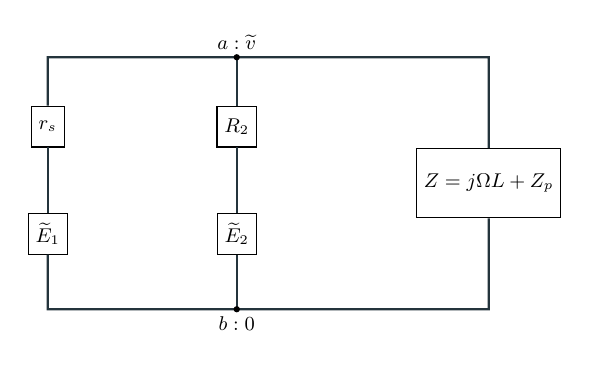
\begin{tikzpicture}[scale=.8,transform shape]
\coordinate (a) at (0,0);\coordinate (b) at (0,-4);
\node[draw,minimum height=.65cm] (rs) at (-3,-1.1) {$r_s$};
\node[draw,minimum height=.65cm] (eone) at (-3,-2.8) {$\widetilde E_1$};
\node[draw,minimum height=.65cm] (rtwo) at (0,-1.1) {$R_2$};
\node[draw,minimum height=.65cm] (etwo) at (0,-2.8) {$\widetilde E_2$};
\node[draw,minimum height=1.1cm] (zz) at (4,-2) {$Z=j\Omega L+Z_p$};
\draw[object] (a)--(-3,0)--(rs.north);\draw[object] (rs.south)--(eone.north);\draw[object] (eone.south)--(-3,-4)--(b);
\draw[object] (a)--(rtwo.north);\draw[object] (rtwo.south)--(etwo.north);\draw[object] (etwo.south)--(b);
\draw[object] (a)--(4,0)--(zz.north);\draw[object] (zz.south)--(4,-4)--(b);
\fill (a) circle(.05) node[above] {$a:\widetilde v$};\fill (b) circle(.05) node[below] {$b:0$};
\end{tikzpicture}
\figcaption{变图电试3.3V4\quad 母线接三个含内阻或阻抗的支路，两电源经结点电压耦合}
\end{minipage}\end{center}

\Needspace{20\baselineskip}
\item 求题设上支路的电流及两电源的平均供给功率，说明电源2的能量作用。
\textbf{解：}变图电试3.3V5取上支路从$a$到$b$为$i_2$，则$i_2=\mathcal E_0(\sin^2x-\cos x)/R$，$x=\omega t$。中支路$i_L=u/R+C\dot u=\mathcal E_0(1-\sin2x-\cos2x)/(2R)$。电源1向$a$送出$i_L+i_2$，电源2的升压方向与$i_2$相反，故两者供给功率分别为$\mathcal E_1(i_L+i_2)$、$-\mathcal E_2i_2$。用$\langle\sin^4x\rangle=3/8$、$\langle\cos^2x\rangle=1/2$与混频项平均为零，得$\langle P_1\rangle=3\mathcal E_0^2/(4R)$、$\langle P_2\rangle=\mathcal E_0^2/(2R)$。$R_2$耗散$7\mathcal E_0^2/(8R)$，加$R_1$的$3\mathcal E_0^2/(8R)$恰等于两源供能总和$5\mathcal E_0^2/(4R)$。
\begin{center}\begin{minipage}{.98\linewidth}\centering
\begin{tikzpicture}[scale=.8,transform shape]
\draw[axis] (0,0)--(10.7,0) node[right] {$\omega t$};
\draw[axis] (0,0)--(0,3.2) node[above] {$iR/\mathcal E_0$};\foreach \y/\lab in {0.12/-1,1.32/0,2.52/1}{\draw[thin] (0,\y)--(-.08,\y) node[left] {$\lab$};}
\node[above] at (5,3.5) {实线上支路$i_2$，虚线中支路$i_L$；均取$a\to b$};
\draw[traj] plot coordinates {(0.000000000,0.120000000) (0.083333333,0.124931421) (0.166666667,0.139685165) (0.250000000,0.164140082) (0.333333333,0.198095605) (0.416666667,0.241273766) (0.500000000,0.293321984) (0.583333333,0.353816593) (0.666666667,0.422267087) (0.750000000,0.498121020) (0.833333333,0.580769515) (0.916666667,0.669553333) (1.000000000,0.763769410) (1.083333333,0.862677832) (1.166666667,0.965509131) (1.250000000,1.071471863) (1.333333333,1.179760350) (1.416666667,1.289562545) (1.500000000,1.400067894) (1.583333333,1.510475144) (1.666666667,1.620000000) (1.750000000,1.727882552) (1.833333333,1.833394392) (1.916666667,1.935845356) (2.000000000,2.034589803) (2.083333333,2.129032388) (2.166666667,2.218633246) (2.250000000,2.302912552) (2.333333333,2.381454405) (2.416666667,2.453909990) (2.500000000,2.520000000) (2.583333333,2.579516285) (2.666666667,2.632322716) (2.750000000,2.678355268) (2.833333333,2.717621304) (2.916666667,2.750198096) (3.000000000,2.776230590) (3.083333333,2.795928435) (3.166666667,2.809562336) (3.250000000,2.817459751) (3.333333333,2.820000000) (3.416666667,2.817608828) (3.500000000,2.810752499) (3.583333333,2.799931484) (3.666666667,2.785673806) (3.750000000,2.768528137) (3.833333333,2.749056713) (3.916666667,2.727828139) (4.000000000,2.705410197) (4.083333333,2.682362696) (4.166666667,2.659230485) (4.250000000,2.636536678) (4.333333333,2.614776185) (4.416666667,2.594409617) (4.500000000,2.575857623) (4.583333333,2.559495749) (4.666666667,2.545649846) (4.750000000,2.534592099) (4.833333333,2.526537714) (4.916666667,2.521642304) (5.000000000,2.520000000) (5.083333333,2.521642304) (5.166666667,2.526537714) (5.250000000,2.534592099) (5.333333333,2.545649846) (5.416666667,2.559495749) (5.500000000,2.575857623) (5.583333333,2.594409617) (5.666666667,2.614776185) (5.750000000,2.636536678) (5.833333333,2.659230485) (5.916666667,2.682362696) (6.000000000,2.705410197) (6.083333333,2.727828139) (6.166666667,2.749056713) (6.250000000,2.768528137) (6.333333333,2.785673806) (6.416666667,2.799931484) (6.500000000,2.810752499) (6.583333333,2.817608828) (6.666666667,2.820000000) (6.750000000,2.817459751) (6.833333333,2.809562336) (6.916666667,2.795928435) (7.000000000,2.776230590) (7.083333333,2.750198096) (7.166666667,2.717621304) (7.250000000,2.678355268) (7.333333333,2.632322716) (7.416666667,2.579516285) (7.500000000,2.520000000) (7.583333333,2.453909990) (7.666666667,2.381454405) (7.750000000,2.302912552) (7.833333333,2.218633246) (7.916666667,2.129032388) (8.000000000,2.034589803) (8.083333333,1.935845356) (8.166666667,1.833394392) (8.250000000,1.727882552) (8.333333333,1.620000000) (8.416666667,1.510475144) (8.500000000,1.400067894) (8.583333333,1.289562545) (8.666666667,1.179760350) (8.750000000,1.071471863) (8.833333333,0.965509131) (8.916666667,0.862677832) (9.000000000,0.763769410) (9.083333333,0.669553333) (9.166666667,0.580769515) (9.250000000,0.498121020) (9.333333333,0.422267087) (9.416666667,0.353816593) (9.500000000,0.293321984) (9.583333333,0.241273766) (9.666666667,0.198095605) (9.750000000,0.164140082) (9.833333333,0.139685165) (9.916666667,0.124931421) (10.000000000,0.120000000)};
\draw[dashed,thick,color=warm] plot coordinates {(0.000000000,1.320000000) (0.083333333,1.260569785) (0.166666667,1.208364425) (0.250000000,1.163955894) (0.333333333,1.127830740) (0.416666667,1.100384758) (0.500000000,1.081918652) (0.583333333,1.072634741) (0.666666667,1.072634741) (0.750000000,1.081918652) (0.833333333,1.100384758) (0.916666667,1.127830740) (1.000000000,1.163955894) (1.083333333,1.208364425) (1.166666667,1.260569785) (1.250000000,1.320000000) (1.333333333,1.386003941) (1.416666667,1.457858454) (1.500000000,1.534776287) (1.583333333,1.615914711) (1.666666667,1.700384758) (1.750000000,1.787260955) (1.833333333,1.875591469) (1.916666667,1.964408531) (2.000000000,2.052739045) (2.083333333,2.139615242) (2.166666667,2.224085289) (2.250000000,2.305223713) (2.333333333,2.382141546) (2.416666667,2.453996059) (2.500000000,2.520000000) (2.583333333,2.579430215) (2.666666667,2.631635575) (2.750000000,2.676044106) (2.833333333,2.712169260) (2.916666667,2.739615242) (3.000000000,2.758081348) (3.083333333,2.767365259) (3.166666667,2.767365259) (3.250000000,2.758081348) (3.333333333,2.739615242) (3.416666667,2.712169260) (3.500000000,2.676044106) (3.583333333,2.631635575) (3.666666667,2.579430215) (3.750000000,2.520000000) (3.833333333,2.453996059) (3.916666667,2.382141546) (4.000000000,2.305223713) (4.083333333,2.224085289) (4.166666667,2.139615242) (4.250000000,2.052739045) (4.333333333,1.964408531) (4.416666667,1.875591469) (4.500000000,1.787260955) (4.583333333,1.700384758) (4.666666667,1.615914711) (4.750000000,1.534776287) (4.833333333,1.457858454) (4.916666667,1.386003941) (5.000000000,1.320000000) (5.083333333,1.260569785) (5.166666667,1.208364425) (5.250000000,1.163955894) (5.333333333,1.127830740) (5.416666667,1.100384758) (5.500000000,1.081918652) (5.583333333,1.072634741) (5.666666667,1.072634741) (5.750000000,1.081918652) (5.833333333,1.100384758) (5.916666667,1.127830740) (6.000000000,1.163955894) (6.083333333,1.208364425) (6.166666667,1.260569785) (6.250000000,1.320000000) (6.333333333,1.386003941) (6.416666667,1.457858454) (6.500000000,1.534776287) (6.583333333,1.615914711) (6.666666667,1.700384758) (6.750000000,1.787260955) (6.833333333,1.875591469) (6.916666667,1.964408531) (7.000000000,2.052739045) (7.083333333,2.139615242) (7.166666667,2.224085289) (7.250000000,2.305223713) (7.333333333,2.382141546) (7.416666667,2.453996059) (7.500000000,2.520000000) (7.583333333,2.579430215) (7.666666667,2.631635575) (7.750000000,2.676044106) (7.833333333,2.712169260) (7.916666667,2.739615242) (8.000000000,2.758081348) (8.083333333,2.767365259) (8.166666667,2.767365259) (8.250000000,2.758081348) (8.333333333,2.739615242) (8.416666667,2.712169260) (8.500000000,2.676044106) (8.583333333,2.631635575) (8.666666667,2.579430215) (8.750000000,2.520000000) (8.833333333,2.453996059) (8.916666667,2.382141546) (9.000000000,2.305223713) (9.083333333,2.224085289) (9.166666667,2.139615242) (9.250000000,2.052739045) (9.333333333,1.964408531) (9.416666667,1.875591469) (9.500000000,1.787260955) (9.583333333,1.700384758) (9.666666667,1.615914711) (9.750000000,1.534776287) (9.833333333,1.457858454) (9.916666667,1.386003941) (10.000000000,1.320000000)};
\node[below] at (0,-.12) {$0$};
\node[below] at (5,-.12) {$\pi$};
\node[below] at (10,-.12) {$2\pi$};
\end{tikzpicture}
\figcaption{变图电试3.3V5\quad 实线上支路$i_2$，虚线中支路$i_L$；均取$a\to b$}
\end{minipage}\end{center}

\Needspace{20\baselineskip}
\item 从$t=0$开始接入题设输入，初始电容电压与电感电流都为零，求全过程的$R_1$电流。
\textbf{解：}变图电试3.3V6的初态为$u(0)=0$、$i_L(0)=0$；结点式又给$\dot u(0)=0$。令$x=\omega t$，将稳态解与自由解相加，$u/\mathcal E_0=(1-\sin2x)/2+e^{-x}(a\cos\sqrt3x+b\sin\sqrt3x)$。由零时刻电压得$a=-1/2$，再由零斜率得$-a+\sqrt3b=1$，所以$b=1/(2\sqrt3)$。最终$i_1=u/R$。图中全过程从零电流、零斜率出发，数个衰减时间后贴近周期稳态；输入及两个储能元件的初态共同确定全过程。
\begin{center}\begin{minipage}{.98\linewidth}\centering
\begin{tikzpicture}[scale=.8,transform shape]
\draw[axis] (0,0)--(10.7,0) node[right] {$\omega t$};
\draw[axis] (0,0)--(0,3.2) node[above] {$i_1R/\mathcal E_0$};\foreach \y/\lab in {0/0,1.4/0.5,2.8/1}{\draw[thin] (0,\y)--(-.08,\y) node[left] {$\lab$};}
\node[above] at (5,3.5) {实线：零储能接通；虚线：周期稳态};
\draw[traj] plot coordinates {(0.000000000,0.000000000) (0.071428571,0.000005715) (0.142857143,0.000089483) (0.214285714,0.000442854) (0.285714286,0.001366810) (0.357142857,0.003255194) (0.428571429,0.006577557) (0.500000000,0.011861707) (0.571428571,0.019676193) (0.642857143,0.030612968) (0.714285714,0.045270480) (0.785714286,0.064237366) (0.857142857,0.088076986) (0.928571429,0.117312938) (1.000000000,0.152415734) (1.071428571,0.193790771) (1.142857143,0.241767707) (1.214285714,0.296591346) (1.285714286,0.358414104) (1.357142857,0.427290109) (1.428571429,0.503170973) (1.500000000,0.585903239) (1.571428571,0.675227503) (1.642857143,0.770779182) (1.714285714,0.872090876) (1.785714286,0.978596268) (1.857142857,1.089635481) (1.928571429,1.204461788) (2.000000000,1.322249582) (2.071428571,1.442103469) (2.142857143,1.563068365) (2.214285714,1.684140448) (2.285714286,1.804278824) (2.357142857,1.922417745) (2.428571429,2.037479232) (2.500000000,2.148385938) (2.571428571,2.254074090) (2.642857143,2.353506353) (2.714285714,2.445684467) (2.785714286,2.529661493) (2.857142857,2.604553538) (2.928571429,2.669550806) (3.000000000,2.723927866) (3.071428571,2.767053002) (3.142857143,2.798396541) (3.214285714,2.817538079) (3.285714286,2.824172500) (3.357142857,2.818114741) (3.428571429,2.799303235) (3.500000000,2.767802008) (3.571428571,2.723801389) (3.642857143,2.667617337) (3.714285714,2.599689393) (3.785714286,2.520577267) (3.857142857,2.430956112) (3.928571429,2.331610520) (4.000000000,2.223427314) (4.071428571,2.107387214) (4.142857143,1.984555456) (4.214285714,1.856071474) (4.285714286,1.723137744) (4.357142857,1.587007921) (4.428571429,1.448974382) (4.500000000,1.310355308) (4.571428571,1.172481454) (4.642857143,1.036682723) (4.714285714,0.904274706) (4.785714286,0.776545320) (4.857142857,0.654741681) (4.928571429,0.540057353) (5.000000000,0.433620109) (5.071428571,0.336480326) (5.142857143,0.249600139) (5.214285714,0.173843461) (5.285714286,0.109966989) (5.357142857,0.058612266) (5.428571429,0.020298906) (5.500000000,-0.004580964) (5.571428571,-0.015766981) (5.642857143,-0.013133490) (5.714285714,0.003308866) (5.785714286,0.033412932) (5.857142857,0.076896212) (5.928571429,0.133343405) (6.000000000,0.202210290) (6.071428571,0.282828918) (6.142857143,0.374414058) (6.214285714,0.476070837) (6.285714286,0.586803497) (6.357142857,0.705525177) (6.428571429,0.831068629) (6.500000000,0.962197750) (6.571428571,1.097619829) (6.642857143,1.235998370) (6.714285714,1.375966374) (6.785714286,1.516139941) (6.857142857,1.655132055) (6.928571429,1.791566415) (7.000000000,1.924091171) (7.071428571,2.051392431) (7.142857143,2.172207392) (7.214285714,2.285336980) (7.285714286,2.389657855) (7.357142857,2.484133668) (7.428571429,2.567825459) (7.500000000,2.639901080) (7.571428571,2.699643563) (7.642857143,2.746458339) (7.714285714,2.779879232) (7.785714286,2.799573177) (7.857142857,2.805343607) (7.928571429,2.797132482) (8.000000000,2.775020922) (8.071428571,2.739228461) (8.142857143,2.690110912) (8.214285714,2.628156865) (8.285714286,2.553982867) (8.357142857,2.468327306) (8.428571429,2.372043090) (8.500000000,2.266089169) (8.571428571,2.151520996) (8.642857143,2.029480029) (8.714285714,1.901182355) (8.785714286,1.767906580) (8.857142857,1.630981083) (8.928571429,1.491770772) (9.000000000,1.351663467) (9.071428571,1.212056059) (9.142857143,1.074340572) (9.214285714,0.939890266) (9.285714286,0.810045931) (9.357142857,0.686102499) (9.428571429,0.569296114) (9.500000000,0.460791786) (9.571428571,0.361671752) (9.642857143,0.272924667) (9.714285714,0.195435721) (9.785714286,0.129977794) (9.857142857,0.077203729) (9.928571429,0.037639806) (10.000000000,0.011680474)};
\draw[dashed,thick,color=warm] plot coordinates {(0.000000000,1.400000000) (0.071428571,1.260233217) (0.142857143,1.121862937) (0.214285714,0.986271711) (0.285714286,0.854814321) (0.357142857,0.728804246) (0.428571429,0.609500537) (0.500000000,0.498095238) (0.571428571,0.395701473) (0.642857143,0.303342327) (0.714285714,0.221940621) (0.785714286,0.152309696) (0.857142857,0.095145280) (0.928571429,0.051018540) (1.000000000,0.020370378) (1.071428571,0.003507019) (1.142857143,0.000596956) (1.214285714,0.011669265) (1.285714286,0.036613317) (1.357142857,0.075179877) (1.428571429,0.126983602) (1.500000000,0.191506887) (1.571428571,0.268105035) (1.642857143,0.356012703) (1.714285714,0.454351547) (1.785714286,0.562138998) (1.857142857,0.678298079) (1.928571429,0.801668168) (2.000000000,0.931016590) (2.071428571,1.065050939) (2.142857143,1.202431989) (2.214285714,1.341787073) (2.285714286,1.481723801) (2.357142857,1.620843972) (2.428571429,1.757757543) (2.500000000,1.891096519) (2.571428571,2.019528621) (2.642857143,2.141770597) (2.714285714,2.256601047) (2.785714286,2.362872623) (2.857142857,2.459523493) (2.928571429,2.545587955) (3.000000000,2.620206081) (3.071428571,2.682632311) (3.142857143,2.732242903) (3.214285714,2.768542165) (3.285714286,2.791167405) (3.357142857,2.799892561) (3.428571429,2.794630452) (3.500000000,2.775433658) (3.571428571,2.742493985) (3.642857143,2.696140555) (3.714285714,2.636836518) (3.785714286,2.565174419) (3.857142857,2.481870283) (3.928571429,2.387756456) (4.000000000,2.283773293) (4.071428571,2.170959760) (4.142857143,2.050443051) (4.214285714,1.923427331) (4.285714286,1.791181697) (4.357142857,1.655027506) (4.428571429,1.516325164) (4.500000000,1.376460539) (4.571428571,1.236831113) (4.642857143,1.098832017) (4.714285714,0.963842091) (4.785714286,0.833210111) (4.857142857,0.708241308) (4.928571429,0.590184330) (5.000000000,0.480218762) (5.071428571,0.379443344) (5.142857143,0.288864991) (5.214285714,0.209388731) (5.285714286,0.141808666) (5.357142857,0.086800033) (5.428571429,0.044912459) (5.500000000,0.016564473) (5.571428571,0.002039316) (5.642857143,0.001482121) (5.714285714,0.014898455) (5.785714286,0.042154265) (5.857142857,0.082977221) (5.928571429,0.136959433) (6.000000000,0.203561529) (6.071428571,0.282118042) (6.142857143,0.371844063) (6.214285714,0.471843078) (6.285714286,0.581115930) (6.357142857,0.698570801) (6.428571429,0.823034121) (6.500000000,0.953262293) (6.571428571,1.087954120) (6.642857143,1.225763807) (6.714285714,1.365314404) (6.785714286,1.505211569) (6.857142857,1.644057494) (6.928571429,1.780464877) (7.000000000,1.913070781) (7.071428571,2.040550251) (7.142857143,2.161629555) (7.214285714,2.275098908) (7.285714286,2.379824563) (7.357142857,2.474760134) (7.428571429,2.558957057) (7.500000000,2.631574064) (7.571428571,2.691885590) (7.642857143,2.739289023) (7.714285714,2.773310722) (7.785714286,2.793610755) (7.857142857,2.799986289) (7.928571429,2.792373623) (8.000000000,2.770848821) (8.071428571,2.735626950) (8.142857143,2.687059936) (8.214285714,2.625633045) (8.285714286,2.551960033) (8.357142857,2.466777017) (8.428571429,2.370935119) (8.500000000,2.265391957) (8.571428571,2.151202085) (8.642857143,2.029506450) (8.714285714,1.901520995) (8.785714286,1.768524508) (8.857142857,1.631845846) (8.928571429,1.492850656) (9.000000000,1.352927734) (9.071428571,1.213475142) (9.142857143,1.075886245) (9.214285714,0.941535785) (9.285714286,0.811766148) (9.357142857,0.687873950) (9.428571429,0.571097079) (9.500000000,0.462602333) (9.571428571,0.363473754) (9.642857143,0.274701803) (9.714285714,0.197173459) (9.785714286,0.131663361) (9.857142857,0.078826063) (9.928571429,0.039189498) (10.000000000,0.013149702)};
\node[below] at (0,-.12) {$0$};
\node[below] at (5,-.12) {$3.5$};
\node[below] at (10,-.12) {$7$};
\end{tikzpicture}
\figcaption{变图电试3.3V6\quad 实线：零储能接通；虚线：周期稳态}
\end{minipage}\end{center}

\Needspace{20\baselineskip}
\item 保持题设$L,C,R$，改变单频输入的频率，求并联端电压幅值最大的频率。
\textbf{解：}变图电试3.3V7令$z=\Omega/(2\omega)$，有$|H|^{-2}=(1-z^2)^2+z^2=1-z^2+z^4$。其导数为$2z(2z^2-1)$，正频率极小点为$z=1/\sqrt2$，于是$\Omega_{\max}=\sqrt2\omega$，最大幅值比$2/\sqrt3$。题设二倍频对应$z=1$，幅值比为1、相位为$-\pi/2$。输出电压幅值最大与实部$1-\Omega^2LC$消失分别对应不同频率，电阻项参与最大值条件。
\begin{center}\begin{minipage}{.98\linewidth}\centering
\begin{tikzpicture}[scale=.8,transform shape]
\draw[axis] (0,0)--(10.7,0) node[right] {$z=\Omega/(2\omega)$};
\draw[axis] (0,0)--(0,3.2) node[above] {$|H|$};\foreach \y/\lab in {0/0,1.25/0.5,2.5/1}{\draw[thin] (0,\y)--(-.08,\y) node[left] {$\lab$};}
\node[above] at (5,3.5) {幅值最大在$z=1/\sqrt2$，二倍频对应$z=1$};
\draw[traj] plot coordinates {(0.000000000,2.500000000) (0.083333333,2.500781128) (0.166666667,2.503123030) (0.250000000,2.507021167) (0.333333333,2.512467649) (0.416666667,2.519450741) (0.500000000,2.527954155) (0.583333333,2.537956115) (0.666666667,2.549428176) (0.750000000,2.562333779) (0.833333333,2.576626506) (0.916666667,2.592248038) (1.000000000,2.609125774) (1.083333333,2.627170106) (1.166666667,2.646271354) (1.250000000,2.666296373) (1.333333333,2.687084877) (1.416666667,2.708445567) (1.500000000,2.730152187) (1.583333333,2.751939721) (1.666666667,2.773500981) (1.750000000,2.794483977) (1.833333333,2.814490499) (1.916666667,2.833076477) (2.000000000,2.849754704) (2.083333333,2.864000558) (2.166666667,2.875261279) (2.250000000,2.882969179) (2.333333333,2.886558915) (2.416666667,2.885488470) (2.500000000,2.879263003) (2.583333333,2.867460135) (2.666666667,2.849754704) (2.750000000,2.825940684) (2.833333333,2.795947917) (2.916666667,2.759851576) (3.000000000,2.717873012) (3.083333333,2.670371559) (3.166666667,2.617827957) (3.250000000,2.560821037) (3.333333333,2.500000000) (3.416666667,2.436054948) (3.500000000,2.369688206) (3.583333333,2.301588552) (3.666666667,2.232409823) (3.750000000,2.162754671) (3.833333333,2.093163578) (3.916666667,2.024108772) (4.000000000,1.955992325) (4.083333333,1.889147579) (4.166666667,1.823843010) (4.250000000,1.760287695) (4.333333333,1.698637695) (4.416666667,1.639002793) (4.500000000,1.581453175) (4.583333333,1.526025774) (4.666666667,1.472730093) (4.750000000,1.421553422) (4.833333333,1.372465413) (4.916666667,1.325422011) (5.000000000,1.280368799) (5.083333333,1.237243794) (5.166666667,1.195979750) (5.250000000,1.156506049) (5.333333333,1.118750218) (5.416666667,1.082639139) (5.500000000,1.048099996) (5.583333333,1.015061014) (5.666666667,0.983452008) (5.750000000,0.953204798) (5.833333333,0.924253497) (5.916666667,0.896534709) (6.000000000,0.869987650) (6.083333333,0.844554212) (6.166666667,0.820178976) (6.250000000,0.796809192) (6.333333333,0.774394733) (6.416666667,0.752888028) (6.500000000,0.732243977) (6.583333333,0.712419862) (6.666666667,0.693375245) (6.750000000,0.675071872) (6.833333333,0.657473564) (6.916666667,0.640546113) (7.000000000,0.624257186) (7.083333333,0.608576217) (7.166666667,0.593474318) (7.250000000,0.578924182) (7.333333333,0.564899992) (7.416666667,0.551377340) (7.500000000,0.538333142) (7.583333333,0.525745566) (7.666666667,0.513593951) (7.750000000,0.501858747) (7.833333333,0.490521444) (7.916666667,0.479564513) (8.000000000,0.468971348) (8.083333333,0.458726211) (8.166666667,0.448814183) (8.250000000,0.439221114) (8.333333333,0.429933580) (8.416666667,0.420938840) (8.500000000,0.412224794) (8.583333333,0.403779951) (8.666666667,0.395593391) (8.750000000,0.387654732) (8.833333333,0.379954101) (8.916666667,0.372482105) (9.000000000,0.365229803) (9.083333333,0.358188681) (9.166666667,0.351350630) (9.250000000,0.344707921) (9.333333333,0.338253188) (9.416666667,0.331979404) (9.500000000,0.325879865) (9.583333333,0.319948173) (9.666666667,0.314178218) (9.750000000,0.308564164) (9.833333333,0.303100436) (9.916666667,0.297781703) (10.000000000,0.292602868)};
\node[below] at (2.357022603955158,-.12) {$1/\sqrt2$};
\node[below] at (3.3333333333333335,-.12) {$1$};
\node[below] at (10,-.12) {$3$};
\end{tikzpicture}
\figcaption{变图电试3.3V7\quad 幅值最大在$z=1/\sqrt2$，二倍频对应$z=1$}
\end{minipage}\end{center}

\Needspace{20\baselineskip}
\item 保持题设参数，母线电压改为$a_0+a_1\cos(2\omega t+\varphi)$，求稳态电流及其各时刻非负的条件。
\textbf{解：}变图电试3.3V8中直流传递系数为1，二倍频系数为$-j$。因此$u=a_0+a_1\cos(2\omega t+\varphi-\pi/2)=a_0+a_1\sin(2\omega t+\varphi)$，$i_1=u/R$。稳态电流的取值范围为$[(a_0-|a_1|)/R,(a_0+|a_1|)/R]$，故各时刻非负恰在$a_0\ge|a_1|$时成立。等号时每周期在最小值处与零轴相切；小于时有一段反向电流。这里的条件针对已达到周期稳态的曲线，任意初态还叠加自由响应。
\begin{center}\begin{minipage}{.98\linewidth}\centering
\begin{tikzpicture}[scale=.8,transform shape]
\draw[axis] (0,0)--(10.7,0) node[right] {$\omega t$};
\draw[axis] (0,0)--(0,3.2) node[above] {$i_1R/U_*$};\foreach \y/\lab in {0.6/0,1.6/0.5,2.6/1}{\draw[thin] (0,\y)--(-.08,\y) node[left] {$\lab$};}
\node[above] at (5,3.5) {实线$a_0>|a_1|$，虚线$a_0<|a_1|$；$\varphi=0$};
\draw[traj] plot coordinates {(0.000000000,2.000000000) (0.083333333,2.052335956) (0.166666667,2.104528463) (0.250000000,2.156434465) (0.333333333,2.207911691) (0.416666667,2.258819045) (0.500000000,2.309016994) (0.583333333,2.358367950) (0.666666667,2.406736643) (0.750000000,2.453990500) (0.833333333,2.500000000) (0.916666667,2.544639035) (1.000000000,2.587785252) (1.083333333,2.629320391) (1.166666667,2.669130606) (1.250000000,2.707106781) (1.333333333,2.743144825) (1.416666667,2.777145961) (1.500000000,2.809016994) (1.583333333,2.838670568) (1.666666667,2.866025404) (1.750000000,2.891006524) (1.833333333,2.913545458) (1.916666667,2.933580426) (2.000000000,2.951056516) (2.083333333,2.965925826) (2.166666667,2.978147601) (2.250000000,2.987688341) (2.333333333,2.994521895) (2.416666667,2.998629535) (2.500000000,3.000000000) (2.583333333,2.998629535) (2.666666667,2.994521895) (2.750000000,2.987688341) (2.833333333,2.978147601) (2.916666667,2.965925826) (3.000000000,2.951056516) (3.083333333,2.933580426) (3.166666667,2.913545458) (3.250000000,2.891006524) (3.333333333,2.866025404) (3.416666667,2.838670568) (3.500000000,2.809016994) (3.583333333,2.777145961) (3.666666667,2.743144825) (3.750000000,2.707106781) (3.833333333,2.669130606) (3.916666667,2.629320391) (4.000000000,2.587785252) (4.083333333,2.544639035) (4.166666667,2.500000000) (4.250000000,2.453990500) (4.333333333,2.406736643) (4.416666667,2.358367950) (4.500000000,2.309016994) (4.583333333,2.258819045) (4.666666667,2.207911691) (4.750000000,2.156434465) (4.833333333,2.104528463) (4.916666667,2.052335956) (5.000000000,2.000000000) (5.083333333,1.947664044) (5.166666667,1.895471537) (5.250000000,1.843565535) (5.333333333,1.792088309) (5.416666667,1.741180955) (5.500000000,1.690983006) (5.583333333,1.641632050) (5.666666667,1.593263357) (5.750000000,1.546009500) (5.833333333,1.500000000) (5.916666667,1.455360965) (6.000000000,1.412214748) (6.083333333,1.370679609) (6.166666667,1.330869394) (6.250000000,1.292893219) (6.333333333,1.256855175) (6.416666667,1.222854039) (6.500000000,1.190983006) (6.583333333,1.161329432) (6.666666667,1.133974596) (6.750000000,1.108993476) (6.833333333,1.086454542) (6.916666667,1.066419574) (7.000000000,1.048943484) (7.083333333,1.034074174) (7.166666667,1.021852399) (7.250000000,1.012311659) (7.333333333,1.005478105) (7.416666667,1.001370465) (7.500000000,1.000000000) (7.583333333,1.001370465) (7.666666667,1.005478105) (7.750000000,1.012311659) (7.833333333,1.021852399) (7.916666667,1.034074174) (8.000000000,1.048943484) (8.083333333,1.066419574) (8.166666667,1.086454542) (8.250000000,1.108993476) (8.333333333,1.133974596) (8.416666667,1.161329432) (8.500000000,1.190983006) (8.583333333,1.222854039) (8.666666667,1.256855175) (8.750000000,1.292893219) (8.833333333,1.330869394) (8.916666667,1.370679609) (9.000000000,1.412214748) (9.083333333,1.455360965) (9.166666667,1.500000000) (9.250000000,1.546009500) (9.333333333,1.593263357) (9.416666667,1.641632050) (9.500000000,1.690983006) (9.583333333,1.741180955) (9.666666667,1.792088309) (9.750000000,1.843565535) (9.833333333,1.895471537) (9.916666667,1.947664044) (10.000000000,2.000000000)};
\draw[dashed,thick,color=warm] plot coordinates {(0.000000000,1.200000000) (0.083333333,1.252335956) (0.166666667,1.304528463) (0.250000000,1.356434465) (0.333333333,1.407911691) (0.416666667,1.458819045) (0.500000000,1.509016994) (0.583333333,1.558367950) (0.666666667,1.606736643) (0.750000000,1.653990500) (0.833333333,1.700000000) (0.916666667,1.744639035) (1.000000000,1.787785252) (1.083333333,1.829320391) (1.166666667,1.869130606) (1.250000000,1.907106781) (1.333333333,1.943144825) (1.416666667,1.977145961) (1.500000000,2.009016994) (1.583333333,2.038670568) (1.666666667,2.066025404) (1.750000000,2.091006524) (1.833333333,2.113545458) (1.916666667,2.133580426) (2.000000000,2.151056516) (2.083333333,2.165925826) (2.166666667,2.178147601) (2.250000000,2.187688341) (2.333333333,2.194521895) (2.416666667,2.198629535) (2.500000000,2.200000000) (2.583333333,2.198629535) (2.666666667,2.194521895) (2.750000000,2.187688341) (2.833333333,2.178147601) (2.916666667,2.165925826) (3.000000000,2.151056516) (3.083333333,2.133580426) (3.166666667,2.113545458) (3.250000000,2.091006524) (3.333333333,2.066025404) (3.416666667,2.038670568) (3.500000000,2.009016994) (3.583333333,1.977145961) (3.666666667,1.943144825) (3.750000000,1.907106781) (3.833333333,1.869130606) (3.916666667,1.829320391) (4.000000000,1.787785252) (4.083333333,1.744639035) (4.166666667,1.700000000) (4.250000000,1.653990500) (4.333333333,1.606736643) (4.416666667,1.558367950) (4.500000000,1.509016994) (4.583333333,1.458819045) (4.666666667,1.407911691) (4.750000000,1.356434465) (4.833333333,1.304528463) (4.916666667,1.252335956) (5.000000000,1.200000000) (5.083333333,1.147664044) (5.166666667,1.095471537) (5.250000000,1.043565535) (5.333333333,0.992088309) (5.416666667,0.941180955) (5.500000000,0.890983006) (5.583333333,0.841632050) (5.666666667,0.793263357) (5.750000000,0.746009500) (5.833333333,0.700000000) (5.916666667,0.655360965) (6.000000000,0.612214748) (6.083333333,0.570679609) (6.166666667,0.530869394) (6.250000000,0.492893219) (6.333333333,0.456855175) (6.416666667,0.422854039) (6.500000000,0.390983006) (6.583333333,0.361329432) (6.666666667,0.333974596) (6.750000000,0.308993476) (6.833333333,0.286454542) (6.916666667,0.266419574) (7.000000000,0.248943484) (7.083333333,0.234074174) (7.166666667,0.221852399) (7.250000000,0.212311659) (7.333333333,0.205478105) (7.416666667,0.201370465) (7.500000000,0.200000000) (7.583333333,0.201370465) (7.666666667,0.205478105) (7.750000000,0.212311659) (7.833333333,0.221852399) (7.916666667,0.234074174) (8.000000000,0.248943484) (8.083333333,0.266419574) (8.166666667,0.286454542) (8.250000000,0.308993476) (8.333333333,0.333974596) (8.416666667,0.361329432) (8.500000000,0.390983006) (8.583333333,0.422854039) (8.666666667,0.456855175) (8.750000000,0.492893219) (8.833333333,0.530869394) (8.916666667,0.570679609) (9.000000000,0.612214748) (9.083333333,0.655360965) (9.166666667,0.700000000) (9.250000000,0.746009500) (9.333333333,0.793263357) (9.416666667,0.841632050) (9.500000000,0.890983006) (9.583333333,0.941180955) (9.666666667,0.992088309) (9.750000000,1.043565535) (9.833333333,1.095471537) (9.916666667,1.147664044) (10.000000000,1.200000000)};
\node[below] at (0,-.12) {$0$};
\node[below] at (5,-.12) {$\pi/2$};
\node[below] at (10,-.12) {$\pi$};
\end{tikzpicture}
\figcaption{变图电试3.3V8\quad $a_1/U_*=0.5,\varphi=0$；实线$a_0/U_*=0.7$，虚线$a_0/U_*=0.3$。}
\end{minipage}\end{center}
\end{enumerate}

\Needspace{13\baselineskip}

\pdfbookmark[2]{第 4 题 三棱柱交流网络与最小补偿电容}{q4}

\section*{第 4 题\quad 三棱柱交流网络与最小补偿电容}\label{q:4}


三棱柱的上三角形为$ABC$、下三角形为$EDF$，对应连接棱为$AE,BD,CF$。九条棱各为相同的电阻$R$与电感$L$串联支路。给定角频率$\omega$下，$\omega L=\sqrt3R$。
\begin{enumerate}
\item 求$A,B$间等效复阻抗的模，答案用$R$表示。
\item 以$A,D$为输入输出端，在每一条支路中串联相同电容$C_1$，使整个网络功率因数为$1/\sqrt2$。求最小$C_1$。
\item 各支路不加电容，仅在网络$AD$外串一个电容$C_2$，使总串联组合功率因数为$1/\sqrt2$，求最小$C_2$。
\end{enumerate}
求最小值时须比较总无功为感性和容性两种可能。


\begin{center}\begin{minipage}{.98\linewidth}\centering
\begin{tikzpicture}[scale=.75,transform shape]

\coordinate (A) at (0,2.8);\coordinate (B) at (3.4,2.8);\coordinate (C) at (1.7,4.5);
\coordinate (E) at (0,0);\coordinate (D) at (3.4,0);\coordinate (F) at (1.7,1.7);
\draw[object] (A)--(B)--(C)--cycle;
\draw[object] (A)--(E)--(D)--(B);
\draw[guide] (E)--(F)--(D);\draw[guide] (C)--(F);
\foreach \p/\pos in {A/above left,B/right,C/above,D/below right,E/left,F/above left}
{\fill (\p) circle (1.5pt);\node[\pos] at (\p) {$\p$};}

\node[align=left] at (7,3) {九条棱各为串联$R,L$\\$z=R+j\sqrt3R$\\$|z|=2R$};
\node[align=left] at (7,.8) {端口一：$A,B$\\端口二：$A,D$};

\end{tikzpicture}
\figcaption{图电试3.4\quad 三棱柱的虚线棱也实际导电，端口选择决定等势结点。}
\end{minipage}\end{center}

\Needspace{8\baselineskip}

\pdfbookmark[3]{题型定位}{q4-h0}

\subsection*{题型定位}

相同复阻抗的空间网络先做拓扑约化，再讨论功率因数。统一的支路因子使结点方程化为实系数网络，端口阻抗为正实数乘同一$z$。求模时保留$|z|$，求补偿时比较相位的感性和容性两支，最小电容由较大的正容抗确定。

\Needspace{8\baselineskip}

\pdfbookmark[3]{知识点}{q4-h1}

\subsection*{知识点}

复阻抗的实部、虚部、模与相位分别对应耗散、储能及电压电流幅值关系。统一支路阻抗可从各结点导纳方程整体提出；等势结点由端口激励的对称性确定。电流分配法结合结点守恒和同端点路径的等电压关系。功率因数为阻抗实部除以模，给定$1/\sqrt2$对应相位$\pm45^\circ$。内部逐支路补偿与外部单电容补偿通过端口拓扑系数相连。

\Needspace{8\baselineskip}

\pdfbookmark[3]{物理图像}{q4-h2}

\subsection*{物理图像}

题图九条棱都导电，虚线只区分前后。解图电试3.4A在$AB$激励下用$C,F$的平均电势移去$CF$，留下两条端口通路。图B按相同比例画出复阻抗的电阻轴、电抗轴与三个状态，向下补偿依次到感性目标、谐振、容性目标。图C为$AD$重新保留$CF$电流，所有下标方向可沿图追踪。

\Needspace{8\baselineskip}

\pdfbookmark[3]{解题入口}{q4-h3}

\subsection*{解题入口}

先写$z$及其模，解释各结点方程中的公共因子怎样消去。第一问用$AB$激励确定零电流棱，再按图A串并联；第二问利用正实拓扑系数保持相位，直接写每支路的功率因数。第三问用$AD$端口的两个独立电流与两条路径方程求$11/15$，再对缩放后的阻抗补偿。

\Needspace{8\baselineskip}

\pdfbookmark[3]{标准解法}{q4-h4}

\subsection*{标准解法}


图电试3.4的九支路阻抗均为
\[
z=R+j\omega L=R(1+j\sqrt3),\qquad |z|=2R.
\]
因为所有支路都是同一个$z$，结点方程可整体约去$1/z$，所以任何指定端口的等效阻抗都等于一个只由拓扑决定的正实系数乘$z$。支路电流的相位由共同复阻抗决定，拓扑约化只处理各支路的实数比例。

具体地，对任一未接电源的结点有$\sum_j(V_i-V_j)/z=0$，约去共同的$1/z$后，只剩连接图的实系数方程。给定总复电流时，电势可写成$\widetilde Iz$乘实数，端口电势差也如此，因此所有拓扑化简均保留复阻抗因子。

第（1）问从$A$入、$B$出时，对称性使$C,F$都在端口平均电势上，交换$A,B$及$E,D$而保持$C,F$不动的反射使电势变成端口电势和减自身，故$V_C=V_F=(V_A+V_B)/2$。连接棱$CF$无电流，可以移除。
\begin{center}\begin{minipage}{.98\linewidth}\centering
\begin{tikzpicture}[scale=.8,transform shape]

\draw[object] (0,0)--(0,2)--(4,2)--(4,0)--cycle;
\node[fill=white] at (2,2) {$2z/3$};
\node[fill=white] at (2,0) {$2z/3$};
\node[fill=white] at (0,1) {$z$};\node[fill=white] at (4,1) {$z$};
\node[above left] at (0,2) {$A$};\node[above right] at (4,2) {$B$};
\node[below left] at (0,0) {$E$};\node[below right] at (4,0) {$D$};
\node[align=center] at (7,1) {$C,F$等势\\$CF$无电流\\两通路并联};
\node at (3.4,-1) {上支路$2z/3$，下绕行支路$8z/3$};

\end{tikzpicture}
\figcaption{解图电试3.4A\quad AB端口下删去零电流棱，各三角形的直接与绕行支路先并联。}
\end{minipage}\end{center}
解图电试3.4A中，上三角形$AB$间的直接支路$z$与经$C$的$2z$并联为$2z/3$；下三角形$ED$间同样化为$2z/3$。端口$AB$还可沿$A\to E\to D\to B$经过串联阻抗$z+2z/3+z=8z/3$，两条通路并联：
\[
\widetilde Z_{AB}
=\frac{2z}{3}\parallel\frac{8z}{3}
=\frac8{15}z.
\]
因此
\[
\boxed{|\widetilde Z_{AB}|=\frac8{15}(2R)
=\frac{16}{15}R}.
\]
$8R/15$为等效有功电阻；题问要求的阻抗模还包含电感电抗，数值为$16R/15$。

第（2）问每支路同加一个$C_1$后，支路阻抗仍处处相同：
\[
z_1=R+j\left(\sqrt3R-\frac1{\omega C_1}\right).
\]
此时整个$AD$阻抗为$kz_1$，$k>0$。功率因数$\Re(kz_1)/|kz_1|$中$k$相消，所以本问可先按每一支路确定相位，故功率因数为
\[
\frac R{\sqrt{R^2+(\sqrt3R-1/\omega C_1)^2}}
=\frac1{\sqrt2}.
\]
\begin{center}\begin{minipage}{.98\linewidth}\centering
\begin{tikzpicture}[scale=.8,transform shape]
\draw[axis] (0,-2.5)--(0,4.3) node[above] {$X/R$};\draw[axis] (0,0)--(5.2,0) node[right] {$\Re z/R$};\draw[guide] (2,-2.2)--(2,3.8);\draw[motion] (0,0)--(2,3.464101615) node[above right] {未补偿$\sqrt3$};\draw[force] (0,0)--(2,2) node[right] {$+1$};\draw[force] (0,0)--(2,-2) node[right] {$-1$};\draw[axis] (4.3,3.3)--(4.3,-1.9) node[midway,right] {容抗增加};\node[below] at (2,0) {$1$};\node at (1.7,-3.2) {横纵同尺度，容性目标所需容抗更大};
\end{tikzpicture}
\figcaption{解图电试3.4B\quad 电抗从正值沿竖直方向降低，两个目标对应相同功率因数}
\end{minipage}\end{center}
从图B中起点的电抗$\sqrt3R$向下移动，功率因数$1/\sqrt2$要求$R^2+X^2=2R^2$。相同的相位余弦对应上下两个目标点，解图电试3.4B中的竖直电抗可以为$+R$或$-R$，于是
\[
\sqrt3R-\frac1{\omega C_1}=\pm R,\qquad
C_1=\frac1{\omega R(\sqrt3\mp1)}.
\]
两个电容都为正，较小者对应电容补偿超过谐振、总支路为容性：
\[
\boxed{C_{1,\min}
=\frac1{(\sqrt3+1)\omega R}}.
\]
总电抗仍为感性的另一个解为$1/[(\sqrt3-1)\omega R]$，它大于容性解，两支正电容比较后选取上式。

第（3）问外接电容前，先求$AD$端口本身的拓扑系数。令总电流复振幅为$\widetilde I$，以从$A$到$E$的电流为$\widetilde I_1$，从$A$到$B$为$\widetilde I_2$。由交换$A,D$且同时交换$B,E$的端口反射对称，$BD$电流也为$\widetilde I_1$，$ED$电流也为$\widetilde I_2$。再由结点守恒，
\[
I_{AC}=I_{FD}=\widetilde I-\widetilde I_1-\widetilde I_2,\quad
I_{CB}=I_{EF}=\widetilde I_1-\widetilde I_2,\quad
I_{CF}=\widetilde I-2\widetilde I_1.
\]
本行各$I$均为复振幅，符号下标规定方向。
\begin{center}\begin{minipage}{.98\linewidth}\centering
\begin{tikzpicture}[scale=.65,transform shape]

\coordinate (A) at (0,2.8);\coordinate (B) at (3.4,2.8);\coordinate (C) at (1.7,4.5);
\coordinate (E) at (0,0);\coordinate (D) at (3.4,0);\coordinate (F) at (1.7,1.7);
\draw[object] (A)--(B)--(C)--cycle;
\draw[object] (A)--(E)--(D)--(B);
\draw[guide] (E)--(F)--(D);\draw[guide] (C)--(F);
\foreach \p/\pos in {A/above left,B/right,C/above,D/below right,E/left,F/above left}
{\fill (\p) circle (1.5pt);\node[\pos] at (\p) {$\p$};}

\draw[motion] (-1,2.8)--(-.1,2.8) node[midway,above] {$\widetilde I$};
\draw[motion] (3.5,0)--(4.4,0) node[midway,below] {$\widetilde I$};
\draw[motion] (0,2.4)--(0,1.3) node[midway,left] {$\widetilde I_1$};
\draw[motion] (.4,2.8)--(2.7,2.8) node[midway,below] {$\widetilde I_2$};
\draw[motion] (3.4,2.4)--(3.4,1.3) node[midway,right] {$\widetilde I_1$};
\draw[motion] (.4,0)--(2.7,0) node[midway,below] {$\widetilde I_2$};
\draw[force] (1.7,3.8)--(1.7,2);
\node[right,color=warm] at (1.8,2.2) {$I_{CF}$};
\node[align=left] at (7.3,3.4) {$I_{AC}=I_{FD}=I-I_1-I_2$\\$I_{CB}=I_{EF}=I_1-I_2$\\$I_{CF}=I-2I_1$\\本图各电流均为复振幅};
\node[align=left] at (7.3,1.1) {比较路径：$ACB$与$AB$\\比较路径：$ACF$与$AEF$};

\end{tikzpicture}
\figcaption{解图电试3.4C\quad AD端口保留CF电流，由结点守恒及两组路径电压求出比例。}
\end{minipage}\end{center}
解图电试3.4C按这些方向标出支路电流。比较$ACB$与$AB$的电压，
\[
(\widetilde I-\widetilde I_1-\widetilde I_2)z
+(\widetilde I_1-\widetilde I_2)z
=\widetilde I_2z,
\]
公共$z$约去后，左端为$\widetilde I-2\widetilde I_2$，故$\widetilde I=3\widetilde I_2$，得到$\widetilde I_2=\widetilde I/3$。再比较$ACF$与$AEF$，
\[
(\widetilde I-\widetilde I_1-\widetilde I_2)z
+(\widetilde I-2\widetilde I_1)z
=\widetilde I_1z+(\widetilde I_1-\widetilde I_2)z,
\]
同样约去$z$，左端为$2\widetilde I-3\widetilde I_1-\widetilde I_2$，右端为$2\widetilde I_1-\widetilde I_2$，因此$2\widetilde I=5\widetilde I_1$，得到$\widetilde I_1=2\widetilde I/5$。于是$AC,FD$各为$4\widetilde I/15$，$CB,EF$各为$\widetilde I/15$，$CF$为$\widetilde I/5$，方向均与图C一致。因此
\[
\widetilde U_{AD}=(\widetilde I_1+\widetilde I_2)z
=\frac{11}{15}\widetilde I z,\qquad
\boxed{\widetilde Z_{AD}=\frac{11}{15}z}.
\]
外串$C_2$后总阻抗为
\[
\widetilde Z_{\rm total}
=\frac{11R}{15}
+j\left(\frac{11\sqrt3R}{15}-\frac1{\omega C_2}\right).
\]
这里电容位于整个$AD$网络外部，其容抗只减一次，而网络的实部和电感电抗均先乘$11/15$。功率因数$1/\sqrt2$要求虚部等于实部的$\pm1$倍，故
\[
\frac1{\omega C_2}
=\frac{11R}{15}(\sqrt3\mp1).
\]
取更大的分母得到最小电容，
\[
\boxed{C_{2,\min}
=\frac{15}{11(\sqrt3+1)\omega R}
=\frac{15}{11}C_{1,\min}}.
\]
两种补偿的结果通过$AD$端口系数关联；前者在全部支路各串联一个电容，后者在整个网络外串联一个电容；外串补偿的容抗乘$11/15$，相应电容乘其倒数$15/11$。


\Needspace{8\baselineskip}

\pdfbookmark[3]{关键洞察}{q4-h5}

\subsection*{关键洞察}

功率因数给相位余弦，相同数值对应电流滞后和超前两种状态。电容越小，容抗越大，因此最小电容可使总电抗越过零点而成为容性。统一支路阻抗时拓扑系数为正实数，只缩放幅值；换端口则改变这个系数与等势关系。外部电容补偿整个端口的电抗，内部电容先按每条支路改变同一因子，两种操作的数量关系由$11/15$给出。

\Needspace{8\baselineskip}

\pdfbookmark[3]{易错点}{q4-h6}

\subsection*{易错点}

$AB$的实部为$8R/15$，模为$16R/15$，使用题问要求的量。$CF$只在$AB$端口下无电流，$AD$下为$\widetilde I/5$。相同支路阻抗保证比例因子共同，支路电流仍由连接和电势差分配。补偿方程保留$X=\pm R_{\rm eq}$，比较两种正电容；外串情形先把电阻和电感电抗都乘$11/15$。

\Needspace{8\baselineskip}

\pdfbookmark[3]{课堂讲解建议}{q4-h7}

\subsection*{课堂讲解建议}

先在复平面标出$R+j\sqrt3R$，让学生读出模$2R$和功率因数$1/2$，再做实系数网络。$AB$与$AD$两种激励各画一遍$CF$，要求说明端点电势怎样决定电流。

第二问先让学生写出带未知正实比例系数$k$的端口阻抗，再在功率因数中约去$k$，解释为何此时无需先求$11/15$。沿图B向下移动电抗，分别读出$X=+R$与$X=-R$所需容抗，再由倒数关系比较电容。最后在图C逐条沿$ACB,AB$与$ACF,AEF$写电压，以结点守恒解释每个复电流系数。

\Needspace{8\baselineskip}

\pdfbookmark[3]{变式训练}{q4-h8}

\subsection*{变式训练}

\begin{enumerate}
\Needspace{20\baselineskip}
\item 目标功率因数改为1，求每支路电容和外串电容，并比较它们与题设两支解的大小。
\textbf{解：}变图电试3.4V1的补偿终点在实轴。每支路要求$\sqrt3R-1/(\omega C_{1,0})=0$，所以$C_{1,0}=1/(\sqrt3\omega R)$；端口$AD$要求$11\sqrt3R/15-1/(\omega C_{2,0})=0$，所以$C_{2,0}=15/(11\sqrt3\omega R)$。对内部补偿，三值满足$1/(\sqrt3+1)<1/\sqrt3<1/(\sqrt3-1)$，统一乘$1/(\omega R)$即可；外串三值再统一乘$15/11$。实轴终点在两种目标相位之间，电容值也位于两解之间。
\begin{center}\begin{minipage}{.98\linewidth}\centering
\begin{tikzpicture}[scale=.8,transform shape]
\draw[axis] (0,-1.8)--(0,3) node[above] {$X$};\draw[axis] (0,0)--(4,0) node[right] {$R$};\draw[motion] (0,0)--(3,0) node[above] {完全补偿};\draw[guide] (3,-1.5)--(3,2.5);\node at (2,-2.4) {$X_L=X_C$};
\end{tikzpicture}
\figcaption{变图电试3.4V1\quad 完全补偿时总阻抗落在正实轴}
\end{minipage}\end{center}

\Needspace{20\baselineskip}
\item 目标改为$0<p<1$，求最小每支路电容与外串电容，并说明感性目标何时也有正解。
\textbf{解：}变图电试3.4V2记$t_p=\sqrt{p^{-2}-1}>0$。由$|X|=Rt_p$得$1/(\omega C_1)=R(\sqrt3\mp t_p)$。容性目标始终给正解，且分母较大，因此$C_{1,\min}=1/[\omega R(\sqrt3+t_p)]$，$C_{2,\min}=15/[11\omega R(\sqrt3+t_p)]$。感性目标的有限正解要求$t_p<\sqrt3$，即$p>1/2$；$p=1/2$时对应不接电容的极限，$p<1/2$时仅容性支给正电容。图中以归一化容抗连续表示这些状态。
\begin{center}\begin{minipage}{.98\linewidth}\centering
\begin{tikzpicture}[scale=.8,transform shape]
\draw[axis] (0,0)--(10.7,0) node[right] {$1/(\omega RC_1)$};
\draw[axis] (0,0)--(0,3.2) node[above] {$p$};\foreach \y/\lab in {0/0,1.5/0.5,3/1}{\draw[thin] (0,\y)--(-.08,\y) node[left] {$\lab$};}
\node[above] at (5,3.5) {功率因数先升至1，再沿容性支下降};
\draw[traj] plot coordinates {(0.000000000,1.500000000) (0.083333333,1.524689769) (0.166666667,1.550058020) (0.250000000,1.576124047) (0.333333333,1.602907016) (0.416666667,1.630425826) (0.500000000,1.658698929) (0.583333333,1.687744129) (0.666666667,1.717578344) (0.750000000,1.748217328) (0.833333333,1.779675346) (0.916666667,1.811964804) (1.000000000,1.845095821) (1.083333333,1.879075734) (1.166666667,1.913908547) (1.250000000,1.949594292) (1.333333333,1.986128317) (1.416666667,2.023500489) (1.500000000,2.061694302) (1.583333333,2.100685895) (1.666666667,2.140442977) (1.750000000,2.180923658) (1.833333333,2.222075206) (1.916666667,2.263832719) (2.000000000,2.306117762) (2.083333333,2.348836972) (2.166666667,2.391880678) (2.250000000,2.435121598) (2.333333333,2.478413649) (2.416666667,2.521590974) (2.500000000,2.564467259) (2.583333333,2.606835437) (2.666666667,2.648467909) (2.750000000,2.689117373) (2.833333333,2.728518388) (2.916666667,2.766389765) (3.000000000,2.802437857) (3.083333333,2.836360795) (3.166666667,2.867853647) (3.250000000,2.896614431) (3.333333333,2.922350843) (3.416666667,2.944787469) (3.500000000,2.963673200) (3.583333333,2.978788510) (3.666666667,2.989952203) (3.750000000,2.997027263) (3.833333333,2.999925432) (3.916666667,2.998610236) (4.000000000,2.993098251) (4.083333333,2.983458525) (4.166666667,2.969810197) (4.250000000,2.952318475) (4.333333333,2.931189223) (4.416666667,2.906662508) (4.500000000,2.879005473) (4.583333333,2.848504936) (4.666666667,2.815460061) (4.750000000,2.780175417) (4.833333333,2.742954679) (4.916666667,2.704095133) (5.000000000,2.663883090) (5.083333333,2.622590241) (5.166666667,2.580470933) (5.250000000,2.537760310) (5.333333333,2.494673216) (5.416666667,2.451403759) (5.500000000,2.408125429) (5.583333333,2.364991642) (5.666666667,2.322136621) (5.750000000,2.279676512) (5.833333333,2.237710650) (5.916666667,2.196322921) (6.000000000,2.155583153) (6.083333333,2.115548497) (6.166666667,2.076264769) (6.250000000,2.037767728) (6.333333333,2.000084273) (6.416666667,1.963233557) (6.500000000,1.927228000) (6.583333333,1.892074217) (6.666666667,1.857773847) (6.750000000,1.824324303) (6.833333333,1.791719432) (6.916666667,1.759950098) (7.000000000,1.729004704) (7.083333333,1.698869637) (7.166666667,1.669529662) (7.250000000,1.640968264) (7.333333333,1.613167943) (7.416666667,1.586110463) (7.500000000,1.559777072) (7.583333333,1.534148687) (7.666666667,1.509206045) (7.750000000,1.484929841) (7.833333333,1.461300831) (7.916666667,1.438299932) (8.000000000,1.415908288) (8.083333333,1.394107341) (8.166666667,1.372878873) (8.250000000,1.352205048) (8.333333333,1.332068443) (8.416666667,1.312452071) (8.500000000,1.293339396) (8.583333333,1.274714346) (8.666666667,1.256561317) (8.750000000,1.238865180) (8.833333333,1.221611276) (8.916666667,1.204785416) (9.000000000,1.188373876) (9.083333333,1.172363387) (9.166666667,1.156741130) (9.250000000,1.141494724) (9.333333333,1.126612218) (9.416666667,1.112082078) (9.500000000,1.097893175) (9.583333333,1.084034775) (9.666666667,1.070496527) (9.750000000,1.057268449) (9.833333333,1.044340916) (9.916666667,1.031704651) (10.000000000,1.019350707)};
\node[below] at (0,-.12) {$0$};
\node[below] at (3.8490017945975046,-.12) {$\sqrt3$};
\node[below] at (10,-.12) {$4.5$};
\end{tikzpicture}
\figcaption{变图电试3.4V2\quad 功率因数先升至1，再沿容性支下降}
\end{minipage}\end{center}

\Needspace{20\baselineskip}
\item 不补偿，端口$AD$接有效电压$U$，求有功、无功及视在功率。
\textbf{解：}变图电试3.4V3中$Z_{AD}=a(1+j\sqrt3)$，$a=11R/15$，故电流有效值$I=U/(2a)$。复功率为$I^2Z$，因此$P=U^2/(4a)=15U^2/(44R)$、$Q=\sqrt3P$、$S=UI=U^2/(2a)=15U^2/(22R)$。三者满足$S^2=P^2+Q^2$，功率因数$P/S=1/2$。图中功率三角形和阻抗三角形同角，因为两者只相差正实倍数$I^2$。
\begin{center}\begin{minipage}{.98\linewidth}\centering
\begin{tikzpicture}[scale=.8,transform shape]
\draw[axis] (0,0)--(4,0) node[right] {$P$};\draw[axis] (0,0)--(0,4) node[above] {$Q$};\draw[motion] (0,0)--(2,3.464101615) node[midway,left] {$S$};\draw[guide] (2,0)--(2,3.464101615);\node[below] at (2,0) {$P$};\node[right] at (2,2) {$Q=\sqrt3P$};
\end{tikzpicture}
\figcaption{变图电试3.4V3\quad 补偿前功率三角形，斜边对应视在功率}
\end{minipage}\end{center}

\Needspace{20\baselineskip}
\item 九条支路统一改为相同的非零复阻抗$z'$，说明两端口阻抗如何变化，并说明仅改一棱时怎样建模。
\textbf{解：}变图电试3.4V4每个内部结点都有$\sum(V_i-V_j)/z'=0$，约去$1/z'$后与单位电阻网络相同。因此指定端口的电压差与总电流仍给$Z_{AB}=8z'/15$、$Z_{AD}=11z'/15$。若只改$CF$，该支路导纳与其余支路的比值随之改变，应在$C,F$结点保留新的导纳。$AB$激励下$C,F$等势仍可使该支路无流，$AD$的电流分配则随新导纳变化。
\begin{center}\begin{minipage}{.98\linewidth}\centering
\begin{tikzpicture}[scale=.65,transform shape]

\coordinate (A) at (0,2.8);\coordinate (B) at (3.4,2.8);\coordinate (C) at (1.7,4.5);
\coordinate (E) at (0,0);\coordinate (D) at (3.4,0);\coordinate (F) at (1.7,1.7);
\draw[object] (A)--(B)--(C)--cycle;
\draw[object] (A)--(E)--(D)--(B);
\draw[guide] (E)--(F)--(D);\draw[guide] (C)--(F);
\foreach \p/\pos in {A/above left,B/right,C/above,D/below right,E/left,F/above left}
{\fill (\p) circle (1.5pt);\node[\pos] at (\p) {$\p$};}

\draw[motion] (-1,2.8)--(-.1,2.8) node[midway,above] {$\widetilde I$};
\draw[motion] (3.5,0)--(4.4,0) node[midway,below] {$\widetilde I$};
\draw[motion] (0,2.4)--(0,1.3) node[midway,left] {$\widetilde I_1$};
\draw[motion] (.4,2.8)--(2.7,2.8) node[midway,below] {$\widetilde I_2$};
\draw[motion] (3.4,2.4)--(3.4,1.3) node[midway,right] {$\widetilde I_1$};
\draw[motion] (.4,0)--(2.7,0) node[midway,below] {$\widetilde I_2$};
\draw[force] (1.7,3.8)--(1.7,2);
\node[right,color=warm] at (1.8,2.2) {$I_{CF}$};
\node[align=left] at (7.3,3.4) {$I_{AC}=I_{FD}=I-I_1-I_2$\\$I_{CB}=I_{EF}=I_1-I_2$\\$I_{CF}=I-2I_1$\\本图各电流均为复振幅};
\node[align=left] at (7.3,1.1) {比较路径：$ACB$与$AB$\\比较路径：$ACF$与$AEF$};

\end{tikzpicture}
\figcaption{变图电试3.4V4\quad AD端口保留CF电流，由结点守恒及两组路径电压求出比例。}
\end{minipage}\end{center}

\Needspace{20\baselineskip}
\item 只把$CF$阻抗改成$kz$，$k>0$，其余八棱仍为$z$，求$AD$等效阻抗。
\textbf{解：}变图电试3.4V5以$D$为零电势，注入总复电流$\widetilde I$，电势单位为$\widetilde Iz$。令各结点无量纲电势为$v_A,v_B,v_C,v_E,v_F$，方程为$3v_A-v_B-v_C-v_E=1$、$3v_B-v_A-v_C=0$、$(2+1/k)v_C-v_A-v_B-v_F/k=0$、$3v_E-v_A-v_F=0$、$(2+1/k)v_F-v_E-v_C/k=0$。消元得到$v_E=1/3$、$v_B=(k+1)/(2k+3)$、$v_F=(k+3)/[3(2k+3)]$、$v_C=(4k+3)/[3(2k+3)]$，故$Z_{AD}=zv_A=(5k+6)z/[3(2k+3)]$。$k=1$恢复$11z/15$，$k\to\infty$为断开$CF$的$5z/6$，$k\to0$为短接的$2z/3$。
\begin{center}\begin{minipage}{.98\linewidth}\centering
\begin{tikzpicture}[scale=.8,transform shape]
\draw[axis] (0,0)--(10.7,0) node[right] {$k$};
\draw[axis] (0,0)--(0,3.2) node[above] {$Z_{AD}/z$};\foreach \y/\lab in {0/0,1.7/0.5,2.72/0.8}{\draw[thin] (0,\y)--(-.08,\y) node[left] {$\lab$};}
\node[above] at (5,3.5) {仅改变$CF$时的端口拓扑系数};
\draw[traj] plot coordinates {(0.100000000,2.284946237) (0.182500000,2.299162084) (0.265000000,2.312659520) (0.347500000,2.325491660) (0.430000000,2.337706511) (0.512500000,2.349347568) (0.595000000,2.360454335) (0.677500000,2.371062769) (0.760000000,2.381205674) (0.842500000,2.390913034) (0.925000000,2.400212314) (1.007500000,2.409128717) (1.090000000,2.417685412) (1.172500000,2.425903735) (1.255000000,2.433803369) (1.337500000,2.441402498) (1.420000000,2.448717949) (1.502500000,2.455765316) (1.585000000,2.462559069) (1.667500000,2.469112658) (1.750000000,2.475438596) (1.832500000,2.481548543) (1.915000000,2.487453374) (1.997500000,2.493163248) (2.080000000,2.498687664) (2.162500000,2.504035513) (2.245000000,2.509215126) (2.327500000,2.514234319) (2.410000000,2.519100431) (2.492500000,2.523820361) (2.575000000,2.528400598) (2.657500000,2.532847253) (2.740000000,2.537166086) (2.822500000,2.541362530) (2.905000000,2.545441716) (2.987500000,2.549408490) (3.070000000,2.553267435) (3.152500000,2.557022890) (3.235000000,2.560678963) (3.317500000,2.564239546) (3.400000000,2.567708333) (3.482500000,2.571088829) (3.565000000,2.574384362) (3.647500000,2.577598095) (3.730000000,2.580733036) (3.812500000,2.583792049) (3.895000000,2.586777858) (3.977500000,2.589693061) (4.060000000,2.592540132) (4.142500000,2.595321433) (4.225000000,2.598039216) (4.307500000,2.600695632) (4.390000000,2.603292738) (4.472500000,2.605832497) (4.555000000,2.608316788) (4.637500000,2.610747409) (4.720000000,2.613126079) (4.802500000,2.615454448) (4.885000000,2.617734094) (4.967500000,2.619966531) (5.050000000,2.622153209) (5.132500000,2.624295522) (5.215000000,2.626394806) (5.297500000,2.628452345) (5.380000000,2.630469372) (5.462500000,2.632447070) (5.545000000,2.634386581) (5.627500000,2.636288998) (5.710000000,2.638155377) (5.792500000,2.639986731) (5.875000000,2.641784038) (5.957500000,2.643548237) (6.040000000,2.645280236) (6.122500000,2.646980908) (6.205000000,2.648651095) (6.287500000,2.650291611) (6.370000000,2.651903237) (6.452500000,2.653486732) (6.535000000,2.655042825) (6.617500000,2.656572221) (6.700000000,2.658075601) (6.782500000,2.659553625) (6.865000000,2.661006927) (6.947500000,2.662436123) (7.030000000,2.663841808) (7.112500000,2.665224557) (7.195000000,2.666584927) (7.277500000,2.667923457) (7.360000000,2.669240669) (7.442500000,2.670537068) (7.525000000,2.671813143) (7.607500000,2.673069369) (7.690000000,2.674306205) (7.772500000,2.675524097) (7.855000000,2.676723476) (7.937500000,2.677904762) (8.020000000,2.679068361) (8.102500000,2.680214666) (8.185000000,2.681344062) (8.267500000,2.682456919) (8.350000000,2.683553598) (8.432500000,2.684634449) (8.515000000,2.685699812) (8.597500000,2.686750018) (8.680000000,2.687785388) (8.762500000,2.688806235) (8.845000000,2.689812861) (8.927500000,2.690805561) (9.010000000,2.691784624) (9.092500000,2.692750327) (9.175000000,2.693702943) (9.257500000,2.694642736) (9.340000000,2.695569962) (9.422500000,2.696484873) (9.505000000,2.697387712) (9.587500000,2.698278716) (9.670000000,2.699158116) (9.752500000,2.700026139) (9.835000000,2.700883002) (9.917500000,2.701728921) (10.000000000,2.702564103)};
\node[below] at (0,-.12) {$0$极限};
\node[below] at (2,-.12) {$1$};
\node[below] at (10,-.12) {$5$};
\end{tikzpicture}
\figcaption{变图电试3.4V5\quad 仅改变$CF$时的端口拓扑系数}
\end{minipage}\end{center}

\Needspace{20\baselineskip}
\item 端口电压有效值$U$保持不变，比较不补偿、题设功率因数及完全补偿时的有功功率。
\textbf{解：}变图电试3.4V6中内部统一补偿或外串理想电容都保持端口有功电阻$a=11R/15$。任一功率因数$p$下$|Z|=a/p$，电流$I=Up/a$，所以$P=I^2a=U^2p^2/a$。不补偿$p=1/2$，题设$p=1/\sqrt2$，完全补偿$p=1$，三种有功功率之比为$1:2:4$。感性与容性两个题设解的$P$相同，无功分别为$+P$与$-P$。这里维持的是端电压；若固定总电流，耗散$I^2a$将保持相同。
\begin{center}\begin{minipage}{.98\linewidth}\centering
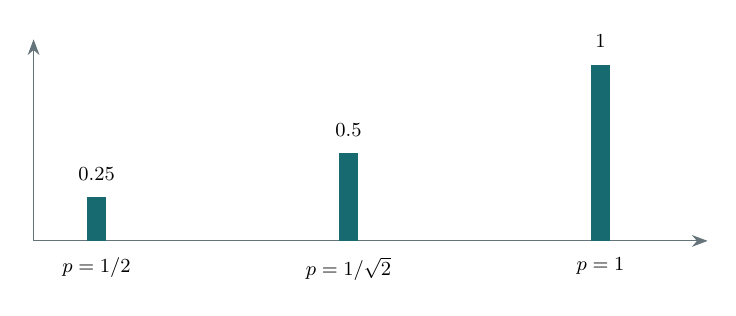
\begin{tikzpicture}[scale=.8,transform shape]
\draw[axis] (0,0)--(10.7,0);
\draw[axis] (0,0)--(0,3.2);
\draw[line width=7pt,color=accent] (1.0,0)--(1.0,0.700000000);
\node[below] at (1.0,-.14) {$p=1/2$};
\node[above] at (1.0,0.840000000) {$ 0.25 $};
\draw[line width=7pt,color=accent] (5.0,0)--(5.0,1.400000000);
\node[below] at (5.0,-.14) {$p=1/\sqrt2$};
\node[above] at (5.0,1.540000000) {$ 0.5 $};
\draw[line width=7pt,color=accent] (9.0,0)--(9.0,2.800000000);
\node[below] at (9.0,-.14) {$p=1$};
\node[above] at (9.0,2.940000000) {$ 1 $};
\end{tikzpicture}
\figcaption{变图电试3.4V6\quad 固定电压下的归一化有功功率$Pa/U^2$}
\end{minipage}\end{center}

\Needspace{20\baselineskip}
\item 把$CF$的阻抗从$z$微调为$(1+\varepsilon)z$，求端口阻抗的一阶变化，并由电流分配解释。
\textbf{解：}变图电试3.4V7中未改动时$I_{CF}=\widetilde I/5$。对实系数网络固定端口电流，耗散变分中电流一阶变化项因结点守恒相消，得到拓扑系数对该棱倍数的导数为$(I_{CF}/\widetilde I)^2=1/25$，故$\delta Z_{AD}=z\varepsilon/25+O(z\varepsilon^2)$。也可对上一变式的$\alpha(k)=(5k+6)/[3(2k+3)]$求导，得$\alpha'(k)=1/(2k+3)^2$，在$k=1$给同值。$AB$下该棱电流为零，端口阻抗保持$8z/15$。
\begin{center}\begin{minipage}{.98\linewidth}\centering
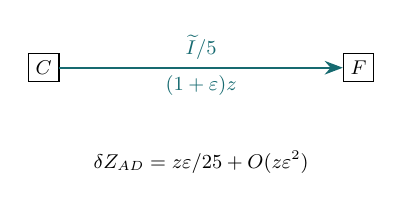
\begin{tikzpicture}[scale=.8,transform shape]
\node[draw] (c) at (0,1) {$C$};\node[draw] (f) at (5,1) {$F$};\draw[motion] (c)--(f) node[midway,above] {$\widetilde I/5$} node[midway,below] {$(1+\varepsilon)z$};\node at (2.5,-.5) {$\delta Z_{AD}=z\varepsilon/25+O(z\varepsilon^2)$};
\end{tikzpicture}
\figcaption{变图电试3.4V7\quad 零阶棱电流决定小改阻的一阶端口变化}
\end{minipage}\end{center}

\Needspace{20\baselineskip}
\item 在设计角频率$\omega_0$取题设最小每支路电容，保持元件参数而改变频率，求功率因数随频率的关系及完全补偿频率。
\textbf{解：}变图电试3.4V8令$\xi=\omega/\omega_0$，有$L=\sqrt3R/\omega_0$、$C_1=1/[(\sqrt3+1)\omega_0R]$。每支路总电抗归一化为$X/R=\sqrt3\xi-(\sqrt3+1)/\xi$，故$p(\xi)=\{1+[\sqrt3\xi-(\sqrt3+1)/\xi]^2\}^{-1/2}$。在设计点$\xi=1$为容性、$p=1/\sqrt2$；完全补偿要求$X=0$，得到$\xi=\sqrt{(\sqrt3+1)/\sqrt3}>1$。频率继续提高后总电抗变为感性，曲线从峰值1再次下降。
\begin{center}\begin{minipage}{.98\linewidth}\centering
\begin{tikzpicture}[scale=.8,transform shape]
\draw[axis] (0,0)--(10.7,0) node[right] {$\xi=\omega/\omega_0$};
\draw[axis] (0,0)--(0,3.2) node[above] {$p$};\foreach \y/\lab in {0/0,1.5/0.5,3/1}{\draw[thin] (0,\y)--(-.08,\y) node[left] {$\lab$};}
\node[above] at (5,3.5) {固定补偿电容后改变频率，峰值对应总电抗为零};
\draw[traj] plot coordinates {(1.000000000,0.284556446) (1.075000000,0.307638969) (1.150000000,0.331119378) (1.225000000,0.355032844) (1.300000000,0.379416186) (1.375000000,0.404308028) (1.450000000,0.429748968) (1.525000000,0.455781753) (1.600000000,0.482451472) (1.675000000,0.509805754) (1.750000000,0.537894987) (1.825000000,0.566772535) (1.900000000,0.596494983) (1.975000000,0.627122384) (2.050000000,0.658718514) (2.125000000,0.691351141) (2.200000000,0.725092297) (2.275000000,0.760018549) (2.350000000,0.796211257) (2.425000000,0.833756832) (2.500000000,0.872746946) (2.575000000,0.913278715) (2.650000000,0.955454800) (2.725000000,0.999383423) (2.800000000,1.045178241) (2.875000000,1.092958042) (2.950000000,1.142846185) (3.025000000,1.194969721) (3.100000000,1.249458066) (3.175000000,1.306441124) (3.250000000,1.366046675) (3.325000000,1.428396836) (3.400000000,1.493603362) (3.475000000,1.561761499) (3.550000000,1.632942074) (3.625000000,1.707181480) (3.700000000,1.784469209) (3.775000000,1.864732653) (3.850000000,1.947819004) (3.925000000,2.033474331) (4.000000000,2.121320344) (4.075000000,2.210829938) (4.150000000,2.301303505) (4.225000000,2.391849019) (4.300000000,2.481370112) (4.375000000,2.568567327) (4.450000000,2.651958188) (4.525000000,2.729921097) (4.600000000,2.800765744) (4.675000000,2.862828641) (4.750000000,2.914586785) (4.825000000,2.954776628) (4.900000000,2.982501355) (4.975000000,2.997308820) (5.050000000,2.999226444) (5.125000000,2.988747225) (5.200000000,2.966770528) (5.275000000,2.934509538) (5.350000000,2.893381834) (5.425000000,2.844899695) (5.500000000,2.790573367) (5.575000000,2.731835251) (5.650000000,2.669987748) (5.725000000,2.606173412) (5.800000000,2.541363610) (5.875000000,2.476360944) (5.950000000,2.411810786) (6.025000000,2.348218020) (6.100000000,2.285965998) (6.175000000,2.225335655) (6.250000000,2.166523496) (6.325000000,2.109657734) (6.400000000,2.054812316) (6.475000000,2.002018789) (6.550000000,1.951276143) (6.625000000,1.902558859) (6.700000000,1.855823381) (6.775000000,1.811013274) (6.850000000,1.768063277) (6.925000000,1.726902467) (7.000000000,1.687456692) (7.075000000,1.649650425) (7.150000000,1.613408152) (7.225000000,1.578655406) (7.300000000,1.545319499) (7.375000000,1.513330051) (7.450000000,1.482619332) (7.525000000,1.453122482) (7.600000000,1.424777628) (7.675000000,1.397525925) (7.750000000,1.371311542) (7.825000000,1.346081609) (7.900000000,1.321786135) (7.975000000,1.298377902) (8.050000000,1.275812353) (8.125000000,1.254047463) (8.200000000,1.233043620) (8.275000000,1.212763490) (8.350000000,1.193171894) (8.425000000,1.174235683) (8.500000000,1.155923620) (8.575000000,1.138206263) (8.650000000,1.121055859) (8.725000000,1.104446236) (8.800000000,1.088352709) (8.875000000,1.072751984) (8.950000000,1.057622072) (9.025000000,1.042942207) (9.100000000,1.028692768) (9.175000000,1.014855211) (9.250000000,1.001411997) (9.325000000,0.988346532) (9.400000000,0.975643106) (9.475000000,0.963286842) (9.550000000,0.951263640) (9.625000000,0.939560134) (9.700000000,0.928163644) (9.775000000,0.917062135) (9.850000000,0.906244180) (9.925000000,0.895698922) (10.000000000,0.885416041)};
\node[below] at (1,-.12) {$1/4$};
\node[below] at (4,-.12) {$1$};
\node[below] at (10,-.12) {$2.5$};
\end{tikzpicture}
\figcaption{变图电试3.4V8\quad 固定补偿电容后改变频率，峰值对应总电抗为零}
\end{minipage}\end{center}
\end{enumerate}

\Needspace{13\baselineskip}

\pdfbookmark[2]{第 5 题 锯齿电源驱动的RC逐周期暂态}{q5}

\section*{第 5 题\quad 锯齿电源驱动的RC逐周期暂态}\label{q:5}


理想电容$C$、电阻$R$、开关$K$和理想电源串联，开始开路且电容不带电。$t=0$闭合开关。电源电动势周期为$T=RC$，在第$n$个完整周期内按
\[
\mathcal E(t)=\mathcal E_0\frac{t-nT}{T},
\qquad nT\le t<(n+1)T,\quad n=0,1,2,\ldots
\]
从零线性升至$\mathcal E_0$，到周期边界瞬间复位至零。
以$Q(t)$表示约定正极板上的带符号电荷，求$Q_N=Q(NT)$、$N=1,2,\ldots$及其$N\to\infty$的极限。给出任一周期内的电荷，并说明电源跳变时哪些量连续、连续时间解最终趋向何种状态。


\begin{center}\begin{minipage}{.98\linewidth}\centering
\begin{tikzpicture}[scale=.7,transform shape]

\draw[object] (0,0)--(0,2)--(1,2);
\draw[object] (1,1.65)--(1,2.35);\draw[object] (1.2,1.65)--(1.2,2.35);
\draw[object] (1.2,2)--(2,2);\draw[object] (2,1.75) rectangle (3.1,2.25);
\draw[object] (3.1,2)--(4,2)--(4,1.2);
\fill (4,1.2) circle (1.5pt);\fill (4,.7) circle (1.5pt);
\draw[object] (4,1.2)--(4.4,.8);\draw[object] (4,.7)--(4,0)--(2.5,0);
\draw[object] (2,0) circle (.5);\draw[object] (1.5,0)--(0,0);
\draw[motion] (2.3,0)--(1.7,0);
\node[above] at (1.1,2.4) {$C$};
\node[above] at (2.55,2.3) {$R$};
\node[right] at (4.5,1) {$K$};\node[below] at (2,-.6) {$\mathcal E(t)$};
\node at (.6,1.4) {$+$};\draw[motion] (.2,3.05)--(1.3,3.05) node[midway,above] {$i=\dot Q$};
\begin{scope}[xshift=6cm,yshift=.3cm]
\draw[axis] (0,0)--(4.2,0) node[right] {$t$};
\draw[axis] (0,0)--(0,2.5) node[above] {$\mathcal E$};
\foreach \n in {0,1,2}{\draw[traj] (\n*1.2,0)--({(\n+1)*1.2},1.8);
\draw[guide] ({(\n+1)*1.2},1.8)--({(\n+1)*1.2},0);}
\node[left] at (0,1.8) {$\mathcal E_0$};
\node[below] at (1.2,0) {$T$};\node[below] at (2.4,0) {$2T$};
\end{scope}

\end{tikzpicture}
\figcaption{图电试3.5\quad 电源在每个周期边界复位，正极板电荷由有限RC电流改变。}
\end{minipage}\end{center}

\Needspace{8\baselineskip}

\pdfbookmark[3]{题型定位}{q5-h0}

\subsection*{题型定位}

周期分段斜坡驱动的$RC$暂态。先在一个连续时间段内解微分方程，再用电荷连续性把末值传给下一段，形成仿射递推。固定相位取样趋于常数，整个波形趋于周期函数；两个结果都应由同一分段通解给出。

\Needspace{8\baselineskip}

\pdfbookmark[3]{知识点}{q5-h1}

\subsection*{知识点}

电阻和电容串联时，$R\dot Q+Q/C=\mathcal E(t)$给一阶线性方程，积分因子处理斜坡驱动。电源每周期复位，局部时间重新计时，而电容电荷由上一周期保留。电荷连续与电流有限跳变分别对应储能状态和瞬时回路电压。仿射递推可通过等比求和或固定点平移求通项，自由响应按$RC$时间常数衰减。周期平均的导数积分为零，电流过零确定电荷的内部极值。

\Needspace{8\baselineskip}

\pdfbookmark[3]{物理图像}{q5-h2}

\subsection*{物理图像}

题图给出充电极性、开关与每周期升压后复位的电源。解图电试3.5A用同一横轴放电源和电荷，电源复位时跳变，电荷曲线的左右端点相接。图B为最终周期电荷，标记复位点和内部最低点；图C为相应电流，复位后从负值逐渐增至正值，在图B最低点过零。

\Needspace{8\baselineskip}

\pdfbookmark[3]{解题入口}{q5-h3}

\subsection*{解题入口}

按题图定义$i=\dot Q$并写回路方程。先解第一周期并由零初值求积分常数，再显式写第二周期的非零初值。找出每周期通解共有的形式后取末值，得到递推与几何级数。把取样极限放回周期初值，求连续的稳定波形和其内部极值。

\Needspace{8\baselineskip}

\pdfbookmark[3]{标准解法}{q5-h4}

\subsection*{标准解法}


图电试3.5中取给电容正极板充电的方向为电流正方向，$i=\dot Q$。回路方程为
\[
Ri+\frac QC=\mathcal E(t),\qquad
\boxed{\dot Q+\frac Q{RC}=\frac{\mathcal E(t)}R}.
\]
电源电动势有限跳变时，电阻限制电流为有限值，故电容电荷与电压连续，$Q(NT^-)=Q(NT^+)$。电流随新回路电压有限跳变，电容电压则保留复位前的数值。

先算第一周期。利用$T=RC$，
\[
\dot Q+\frac QT=\frac{C\mathcal E_0}{T^2}t.
\]
乘积分因子$e^{t/T}$，
\[
\frac d{dt}(Qe^{t/T})
=\frac{C\mathcal E_0}{T^2}t e^{t/T}.
\]
由于
\[
\int t e^{t/T}dt=T(t-T)e^{t/T},
\]
因此积分后$Q=C\mathcal E_0(t/T-1)+Ae^{-t/T}$。在$t=0$，右端为$-C\mathcal E_0+A$，结合$Q(0)=0$求得$A=C\mathcal E_0$，得到
\[
\boxed{Q(t)=C\mathcal E_0\left(\frac tT-1+e^{-t/T}\right)}
\quad(0\le t<T),\qquad
Q_1=\frac{C\mathcal E_0}{e}.
\]
\begin{center}\begin{minipage}{.98\linewidth}\centering
\begin{tikzpicture}[scale=.8,transform shape]
\draw[axis] (0,0)--(10.7,0) node[right] {$t/T$};
\draw[axis] (0,0)--(0,3.2) node[above] {$Q/(C\mathcal E_0)$};\foreach \y/\lab in {0/0,1.4/0.5,2.8/1}{\draw[thin] (0,\y)--(-.08,\y) node[left] {$\lab$};}
\node[above] at (5,3.5) {电荷连续；虚线为同刻电源$\mathcal E/\mathcal E_0$};
\draw[traj] plot coordinates {(0.000000000,0.000000000) (0.031250000,0.000217841) (0.062500000,0.000867754) (0.093750000,0.001944370) (0.125000000,0.003442389) (0.156250000,0.005356576) (0.187500000,0.007681762) (0.218750000,0.010412841) (0.250000000,0.013544771) (0.281250000,0.017072572) (0.312500000,0.020991327) (0.343750000,0.025296180) (0.375000000,0.029982334) (0.406250000,0.035045053) (0.437500000,0.040479658) (0.468750000,0.046281531) (0.500000000,0.052446109) (0.531250000,0.058968886) (0.562500000,0.065845413) (0.593750000,0.073071295) (0.625000000,0.080642193) (0.656250000,0.088553820) (0.687500000,0.096801945) (0.718750000,0.105382387) (0.750000000,0.114291018) (0.781250000,0.123523761) (0.812500000,0.133076590) (0.843750000,0.142945529) (0.875000000,0.153126651) (0.906250000,0.163616078) (0.937500000,0.174409981) (0.968750000,0.185504576) (1.000000000,0.196896129) (1.031250000,0.208580951) (1.062500000,0.220555398) (1.093750000,0.232815874) (1.125000000,0.245358825) (1.156250000,0.258180741) (1.187500000,0.271278158) (1.218750000,0.284647653) (1.250000000,0.298285847) (1.281250000,0.312189402) (1.312500000,0.326355020) (1.343750000,0.340779448) (1.375000000,0.355459469) (1.406250000,0.370391909) (1.437500000,0.385573633) (1.468750000,0.401001543) (1.500000000,0.416672581) (1.531250000,0.432583728) (1.562500000,0.448732000) (1.593750000,0.465114452) (1.625000000,0.481728175) (1.656250000,0.498570296) (1.687500000,0.515637978) (1.718750000,0.532928418) (1.750000000,0.550438851) (1.781250000,0.568166542) (1.812500000,0.586108793) (1.843750000,0.604262939) (1.875000000,0.622626348) (1.906250000,0.641196419) (1.937500000,0.659970587) (1.968750000,0.678946315) (2.000000000,0.698121100) (2.031250000,0.717492468) (2.062500000,0.737057979) (2.093750000,0.756815220) (2.125000000,0.776761809) (2.156250000,0.796895395) (2.187500000,0.817213655) (2.218750000,0.837714294) (2.250000000,0.858395047) (2.281250000,0.879253677) (2.312500000,0.900287973) (2.343750000,0.921495755) (2.375000000,0.942874866) (2.406250000,0.964423178) (2.437500000,0.986138590) (2.468750000,1.008019026) (2.500000000,1.030062435) (2.531250000,1.017484636) (2.562500000,1.005497857) (2.593750000,0.994094757) (2.625000000,0.983268086) (2.656250000,0.973010683) (2.687500000,0.963315477) (2.718750000,0.954175483) (2.750000000,0.945583805) (2.781250000,0.937533631) (2.812500000,0.930018236) (2.843750000,0.923030975) (2.875000000,0.916565288) (2.906250000,0.910614697) (2.937500000,0.905172801) (2.968750000,0.900233283) (3.000000000,0.895789902) (3.031250000,0.891836494) (3.062500000,0.888366973) (3.093750000,0.885375329) (3.125000000,0.882855624) (3.156250000,0.880801996) (3.187500000,0.879208656) (3.218750000,0.878069886) (3.250000000,0.877380038) (3.281250000,0.877133537) (3.312500000,0.877324876) (3.343750000,0.877948614) (3.375000000,0.878999381) (3.406250000,0.880471872) (3.437500000,0.882360849) (3.468750000,0.884661137) (3.500000000,0.887367628) (3.531250000,0.890475275) (3.562500000,0.893979095) (3.593750000,0.897874167) (3.625000000,0.902155631) (3.656250000,0.906818687) (3.687500000,0.911858594) (3.718750000,0.917270671) (3.750000000,0.923050296) (3.781250000,0.929192901) (3.812500000,0.935693979) (3.843750000,0.942549077) (3.875000000,0.949753796) (3.906250000,0.957303793) (3.937500000,0.965194780) (3.968750000,0.973422521) (4.000000000,0.981982831) (4.031250000,0.990871581) (4.062500000,1.000084690) (4.093750000,1.009618129) (4.125000000,1.019467919) (4.156250000,1.029630130) (4.187500000,1.040100880) (4.218750000,1.050876338) (4.250000000,1.061952718) (4.281250000,1.073326282) (4.312500000,1.084993338) (4.343750000,1.096950241) (4.375000000,1.109193389) (4.406250000,1.121719228) (4.437500000,1.134524245) (4.468750000,1.147604973) (4.500000000,1.160957987) (4.531250000,1.174579903) (4.562500000,1.188467382) (4.593750000,1.202617126) (4.625000000,1.217025875) (4.656250000,1.231690413) (4.687500000,1.246607562) (4.718750000,1.261774185) (4.750000000,1.277187181) (4.781250000,1.292843491) (4.812500000,1.308740093) (4.843750000,1.324874000) (4.875000000,1.341242266) (4.906250000,1.357841979) (4.937500000,1.374670264) (4.968750000,1.391724282) (5.000000000,1.409001228) (5.031250000,1.391716175) (5.062500000,1.375080618) (5.093750000,1.359086487) (5.125000000,1.343725816) (5.156250000,1.328990735) (5.187500000,1.314873474) (5.218750000,1.301366356) (5.250000000,1.288461804) (5.281250000,1.276152332) (5.312500000,1.264430547) (5.343750000,1.253289150) (5.375000000,1.242720930) (5.406250000,1.232718768) (5.437500000,1.223275632) (5.468750000,1.214384577) (5.500000000,1.206038745) (5.531250000,1.198231365) (5.562500000,1.190955746) (5.593750000,1.184205283) (5.625000000,1.177973453) (5.656250000,1.172253812) (5.687500000,1.167040000) (5.718750000,1.162325731) (5.750000000,1.158104801) (5.781250000,1.154371081) (5.812500000,1.151118519) (5.843750000,1.148341138) (5.875000000,1.146033035) (5.906250000,1.144188381) (5.937500000,1.142801419) (5.968750000,1.141866462) (6.000000000,1.141377897) (6.031250000,1.141330178) (6.062500000,1.141717829) (6.093750000,1.142535441) (6.125000000,1.143777673) (6.156250000,1.145439252) (6.187500000,1.147514967) (6.218750000,1.149999673) (6.250000000,1.152888292) (6.281250000,1.156175804) (6.312500000,1.159857255) (6.343750000,1.163927752) (6.375000000,1.168382461) (6.406250000,1.173216609) (6.437500000,1.178425484) (6.468750000,1.184004430) (6.500000000,1.189948850) (6.531250000,1.196254205) (6.562500000,1.202916010) (6.593750000,1.209929838) (6.625000000,1.217291316) (6.656250000,1.224996125) (6.687500000,1.233040000) (6.718750000,1.241418729) (6.750000000,1.250128154) (6.781250000,1.259164165) (6.812500000,1.268522706) (6.843750000,1.278199770) (6.875000000,1.288191401) (6.906250000,1.298493690) (6.937500000,1.309102780) (6.968750000,1.320014859) (7.000000000,1.331226162) (7.031250000,1.342732973) (7.062500000,1.354531622) (7.093750000,1.366618482) (7.125000000,1.378989974) (7.156250000,1.391642561) (7.187500000,1.404572753) (7.218750000,1.417777100) (7.250000000,1.431252197) (7.281250000,1.444994681) (7.312500000,1.459001230) (7.343750000,1.473268564) (7.375000000,1.487793443) (7.406250000,1.502572668) (7.437500000,1.517603079) (7.468750000,1.532881557) (7.500000000,1.548405020) (7.531250000,1.529388265) (7.562500000,1.511042517) (7.593750000,1.493359441) (7.625000000,1.476330804) (7.656250000,1.459948478) (7.687500000,1.444204433) (7.718750000,1.429090741) (7.750000000,1.414599571) (7.781250000,1.400723190) (7.812500000,1.387453961) (7.843750000,1.374784342) (7.875000000,1.362706885) (7.906250000,1.351214234) (7.937500000,1.340299123) (7.968750000,1.329954379) (8.000000000,1.320172917) (8.031250000,1.310947738) (8.062500000,1.302271934) (8.093750000,1.294138679) (8.125000000,1.286541235) (8.156250000,1.279472944) (8.187500000,1.272927234) (8.218750000,1.266897612) (8.250000000,1.261377670) (8.281250000,1.256361073) (8.312500000,1.251841572) (8.343750000,1.247812989) (8.375000000,1.244269227) (8.406250000,1.241204263) (8.437500000,1.238612150) (8.468750000,1.236487014) (8.500000000,1.234823053) (8.531250000,1.233614540) (8.562500000,1.232855815) (8.593750000,1.232541293) (8.625000000,1.232665455) (8.656250000,1.233222852) (8.687500000,1.234208101) (8.718750000,1.235615889) (8.750000000,1.237440965) (8.781250000,1.239678147) (8.812500000,1.242322316) (8.843750000,1.245368415) (8.875000000,1.248811452) (8.906250000,1.252646495) (8.937500000,1.256868676) (8.968750000,1.261473185) (9.000000000,1.266455273) (9.031250000,1.271810250) (9.062500000,1.277533483) (9.093750000,1.283620397) (9.125000000,1.290066476) (9.156250000,1.296867258) (9.187500000,1.304018335) (9.218750000,1.311515358) (9.250000000,1.319354028) (9.281250000,1.327530101) (9.312500000,1.336039387) (9.343750000,1.344877745) (9.375000000,1.354041089) (9.406250000,1.363525381) (9.437500000,1.373326634) (9.468750000,1.383440911) (9.500000000,1.393864323) (9.531250000,1.404593031) (9.562500000,1.415623241) (9.593750000,1.426951209) (9.625000000,1.438573236) (9.656250000,1.450485668) (9.687500000,1.462684899) (9.718750000,1.475167365) (9.750000000,1.487929549) (9.781250000,1.500967976) (9.812500000,1.514279213) (9.843750000,1.527859873) (9.875000000,1.541706608) (9.906250000,1.555816113) (9.937500000,1.570185124) (9.968750000,1.584810417) (10.000000000,1.599688809)};
\node[below] at (0,-.12) {$0$};
\node[below] at (2.5,-.12) {$1$};
\node[below] at (5,-.12) {$2$};
\node[below] at (7.5,-.12) {$3$};
\node[below] at (10,-.12) {$4$};
\draw[dashed,color=warm] plot coordinates {(0.000000000,0.000000000) (0.062500000,0.070000000) (0.125000000,0.140000000) (0.187500000,0.210000000) (0.250000000,0.280000000) (0.312500000,0.350000000) (0.375000000,0.420000000) (0.437500000,0.490000000) (0.500000000,0.560000000) (0.562500000,0.630000000) (0.625000000,0.700000000) (0.687500000,0.770000000) (0.750000000,0.840000000) (0.812500000,0.910000000) (0.875000000,0.980000000) (0.937500000,1.050000000) (1.000000000,1.120000000) (1.062500000,1.190000000) (1.125000000,1.260000000) (1.187500000,1.330000000) (1.250000000,1.400000000) (1.312500000,1.470000000) (1.375000000,1.540000000) (1.437500000,1.610000000) (1.500000000,1.680000000) (1.562500000,1.750000000) (1.625000000,1.820000000) (1.687500000,1.890000000) (1.750000000,1.960000000) (1.812500000,2.030000000) (1.875000000,2.100000000) (1.937500000,2.170000000) (2.000000000,2.240000000) (2.062500000,2.310000000) (2.125000000,2.380000000) (2.187500000,2.450000000) (2.250000000,2.520000000) (2.312500000,2.590000000) (2.375000000,2.660000000) (2.437500000,2.730000000) (2.500000000,2.800000000)};
\draw[dashed,color=warm] plot coordinates {(2.500000000,0.000000000) (2.562500000,0.070000000) (2.625000000,0.140000000) (2.687500000,0.210000000) (2.750000000,0.280000000) (2.812500000,0.350000000) (2.875000000,0.420000000) (2.937500000,0.490000000) (3.000000000,0.560000000) (3.062500000,0.630000000) (3.125000000,0.700000000) (3.187500000,0.770000000) (3.250000000,0.840000000) (3.312500000,0.910000000) (3.375000000,0.980000000) (3.437500000,1.050000000) (3.500000000,1.120000000) (3.562500000,1.190000000) (3.625000000,1.260000000) (3.687500000,1.330000000) (3.750000000,1.400000000) (3.812500000,1.470000000) (3.875000000,1.540000000) (3.937500000,1.610000000) (4.000000000,1.680000000) (4.062500000,1.750000000) (4.125000000,1.820000000) (4.187500000,1.890000000) (4.250000000,1.960000000) (4.312500000,2.030000000) (4.375000000,2.100000000) (4.437500000,2.170000000) (4.500000000,2.240000000) (4.562500000,2.310000000) (4.625000000,2.380000000) (4.687500000,2.450000000) (4.750000000,2.520000000) (4.812500000,2.590000000) (4.875000000,2.660000000) (4.937500000,2.730000000) (5.000000000,2.800000000)};
\draw[dashed,color=warm] plot coordinates {(5.000000000,0.000000000) (5.062500000,0.070000000) (5.125000000,0.140000000) (5.187500000,0.210000000) (5.250000000,0.280000000) (5.312500000,0.350000000) (5.375000000,0.420000000) (5.437500000,0.490000000) (5.500000000,0.560000000) (5.562500000,0.630000000) (5.625000000,0.700000000) (5.687500000,0.770000000) (5.750000000,0.840000000) (5.812500000,0.910000000) (5.875000000,0.980000000) (5.937500000,1.050000000) (6.000000000,1.120000000) (6.062500000,1.190000000) (6.125000000,1.260000000) (6.187500000,1.330000000) (6.250000000,1.400000000) (6.312500000,1.470000000) (6.375000000,1.540000000) (6.437500000,1.610000000) (6.500000000,1.680000000) (6.562500000,1.750000000) (6.625000000,1.820000000) (6.687500000,1.890000000) (6.750000000,1.960000000) (6.812500000,2.030000000) (6.875000000,2.100000000) (6.937500000,2.170000000) (7.000000000,2.240000000) (7.062500000,2.310000000) (7.125000000,2.380000000) (7.187500000,2.450000000) (7.250000000,2.520000000) (7.312500000,2.590000000) (7.375000000,2.660000000) (7.437500000,2.730000000) (7.500000000,2.800000000)};
\draw[dashed,color=warm] plot coordinates {(7.500000000,0.000000000) (7.562500000,0.070000000) (7.625000000,0.140000000) (7.687500000,0.210000000) (7.750000000,0.280000000) (7.812500000,0.350000000) (7.875000000,0.420000000) (7.937500000,0.490000000) (8.000000000,0.560000000) (8.062500000,0.630000000) (8.125000000,0.700000000) (8.187500000,0.770000000) (8.250000000,0.840000000) (8.312500000,0.910000000) (8.375000000,0.980000000) (8.437500000,1.050000000) (8.500000000,1.120000000) (8.562500000,1.190000000) (8.625000000,1.260000000) (8.687500000,1.330000000) (8.750000000,1.400000000) (8.812500000,1.470000000) (8.875000000,1.540000000) (8.937500000,1.610000000) (9.000000000,1.680000000) (9.062500000,1.750000000) (9.125000000,1.820000000) (9.187500000,1.890000000) (9.250000000,1.960000000) (9.312500000,2.030000000) (9.375000000,2.100000000) (9.437500000,2.170000000) (9.500000000,2.240000000) (9.562500000,2.310000000) (9.625000000,2.380000000) (9.687500000,2.450000000) (9.750000000,2.520000000) (9.812500000,2.590000000) (9.875000000,2.660000000) (9.937500000,2.730000000) (10.000000000,2.800000000)};
\end{tikzpicture}
\figcaption{解图电试3.5A\quad 电荷连续；虚线为同刻电源$\mathcal E/\mathcal E_0$}
\end{minipage}\end{center}
第一周期末值通过有限电流积分传给第二周期。令$t'=t-T$，$0\le t'<T$，方程仍是$\mathrm dQ/\mathrm dt'+Q/T=C\mathcal E_0t'/T^2$，通解为$Q=C\mathcal E_0(t'/T-1)+A'e^{-t'/T}$。在$t'=0$时取$Q=Q_1=C\mathcal E_0/e$，使$A'=C\mathcal E_0(1+e^{-1})$，于是第二周期
\[
Q=C\mathcal E_0\left(\frac{t'}T-1\right)+C\mathcal E_0(1+e^{-1})e^{-t'/T}.
\]
取$t'\to T^-$得$Q_2=C\mathcal E_0(e^{-1}+e^{-2})$，第二次复位仍保留这个末值。这两个周期显示了分段时间的重新计时与状态的连续传递。

解图电试3.5A将电源复位点与连续的$Q$曲线放在同一时间轴上。第$n$周期从$t=nT$开始，令$s=t-nT$、$0\le s<T$，初始电荷为$Q_n$。方程形式不变，只需使用新的初值：
\[
\boxed{Q(nT+s)
=C\mathcal E_0\left(\frac sT-1\right)
+(Q_n+C\mathcal E_0)e^{-s/T}}.
\]
取$s\to T^-$，用电荷连续性得到
\[
Q_{n+1}=e^{-1}Q_n+\frac{C\mathcal E_0}{e}.
\]
例如
\[
Q_2=C\mathcal E_0(e^{-1}+e^{-2}),\qquad
Q_3=C\mathcal E_0(e^{-1}+e^{-2}+e^{-3}).
\]
递推$Q_0=0$，每次迭代使已有项再乘$e^{-1}$，同时新添$C\mathcal E_0e^{-1}$，故第$N$次有$e^{-1}$到$e^{-N}$共$N$项。令公比$a=e^{-1}$，求和为$a(1-a^N)/(1-a)=(1-e^{-N})/(e-1)$，对等比数列求和，
\[
Q_N=C\mathcal E_0\sum_{k=1}^Ne^{-k}
=\boxed{\frac{1-e^{-N}}{e-1}C\mathcal E_0}.
\]
于是
\[
\boxed{\lim_{N\to\infty}Q_N
=Q_*=\frac{C\mathcal E_0}{e-1}}.
\]
误差$Q_*-Q_N=Q_*e^{-N}$，每多一个周期便再乘$e^{-1}$。这一极限描述每次复位时刻的电荷；周期内的连续波形由同一通解保留。
\begin{center}\begin{minipage}{.98\linewidth}\centering
\begin{tikzpicture}[scale=.8,transform shape]
\draw[axis] (0,0)--(10.7,0) node[right] {$s/T$};
\draw[axis] (0,0)--(0,3.2) node[above] {$Q_{\rm per}/(C\mathcal E_0)$};\foreach \y/\lab in {1.92/0.4,2.4/0.5,2.88/0.6}{\draw[thin] (0,\y)--(-.08,\y) node[left] {$\lab$};}
\node[above] at (5,3.5) {两端$1/(e-1)$，内部最低点$\ln[e/(e-1)]$};
\draw[traj] plot coordinates {(0.000000000,2.793488193) (0.083333333,2.770472057) (0.166666667,2.747978873) (0.250000000,2.726004301) (0.333333333,2.704544039) (0.416666667,2.683593817) (0.500000000,2.663149404) (0.583333333,2.643206601) (0.666666667,2.623761245) (0.750000000,2.604809210) (0.833333333,2.586346399) (0.916666667,2.568368755) (1.000000000,2.550872250) (1.083333333,2.533852892) (1.166666667,2.517306721) (1.250000000,2.501229810) (1.333333333,2.485618265) (1.416666667,2.470468224) (1.500000000,2.455775857) (1.583333333,2.441537365) (1.666666667,2.427748984) (1.750000000,2.414406976) (1.833333333,2.401507638) (1.916666667,2.389047296) (2.000000000,2.377022307) (2.083333333,2.365429058) (2.166666667,2.354263966) (2.250000000,2.343523479) (2.333333333,2.333204072) (2.416666667,2.323302251) (2.500000000,2.313814551) (2.583333333,2.304737535) (2.666666667,2.296067794) (2.750000000,2.287801949) (2.833333333,2.279936649) (2.916666667,2.272468569) (3.000000000,2.265394412) (3.083333333,2.258710910) (3.166666667,2.252414821) (3.250000000,2.246502929) (3.333333333,2.240972047) (3.416666667,2.235819012) (3.500000000,2.231040689) (3.583333333,2.226633968) (3.666666667,2.222595766) (3.750000000,2.218923024) (3.833333333,2.215612709) (3.916666667,2.212661813) (4.000000000,2.210067355) (4.083333333,2.207826376) (4.166666667,2.205935942) (4.250000000,2.204393144) (4.333333333,2.203195098) (4.416666667,2.202338943) (4.500000000,2.201821841) (4.583333333,2.201640978) (4.666666667,2.201793565) (4.750000000,2.202276834) (4.833333333,2.203088040) (4.916666667,2.204224463) (5.000000000,2.205683403) (5.083333333,2.207462184) (5.166666667,2.209558152) (5.250000000,2.211968675) (5.333333333,2.214691141) (5.416666667,2.217722963) (5.500000000,2.221061573) (5.583333333,2.224704425) (5.666666667,2.228648995) (5.750000000,2.232892777) (5.833333333,2.237433291) (5.916666667,2.242268072) (6.000000000,2.247394679) (6.083333333,2.252810690) (6.166666667,2.258513703) (6.250000000,2.264501338) (6.333333333,2.270771230) (6.416666667,2.277321040) (6.500000000,2.284148442) (6.583333333,2.291251134) (6.666666667,2.298626831) (6.750000000,2.306273268) (6.833333333,2.314188198) (6.916666667,2.322369392) (7.000000000,2.330814641) (7.083333333,2.339521754) (7.166666667,2.348488557) (7.250000000,2.357712896) (7.333333333,2.367192633) (7.416666667,2.376925648) (7.500000000,2.386909841) (7.583333333,2.397143126) (7.666666667,2.407623436) (7.750000000,2.418348721) (7.833333333,2.429316949) (7.916666667,2.440526103) (8.000000000,2.451974184) (8.083333333,2.463659209) (8.166666667,2.475579211) (8.250000000,2.487732241) (8.333333333,2.500116365) (8.416666667,2.512729665) (8.500000000,2.525570239) (8.583333333,2.538636202) (8.666666667,2.551925682) (8.750000000,2.565436825) (8.833333333,2.579167791) (8.916666667,2.593116756) (9.000000000,2.607281911) (9.083333333,2.621661462) (9.166666667,2.636253629) (9.250000000,2.651056649) (9.333333333,2.666068771) (9.416666667,2.681288260) (9.500000000,2.696713395) (9.583333333,2.712342470) (9.666666667,2.728173792) (9.750000000,2.744205683) (9.833333333,2.760436478) (9.916666667,2.776864527) (10.000000000,2.793488193)};
\node[below] at (0,-.12) {$0$};
\node[below] at (4.58675145387082,-.12) {$x_m$};
\node[below] at (10,-.12) {$1$};
\end{tikzpicture}
\figcaption{解图电试3.5B\quad 两端$1/(e-1)$，内部最低点$\ln[e/(e-1)]$}
\end{minipage}\end{center}
解图电试3.5B中，稳定后的一个周期电荷为
\[
\boxed{Q_{\rm per}(s)=C\mathcal E_0
\left[\frac sT-1+\frac e{e-1}e^{-s/T}\right]},
\qquad 0\le s<T.
\]
它在两端都等于$Q_*$，周期内却有变化。由
\[
i_{\rm per}(s)
=\frac{\mathcal E_0}{R}
\left[1-\frac e{e-1}e^{-s/T}\right],
\]
\begin{center}\begin{minipage}{.98\linewidth}\centering
\begin{tikzpicture}[scale=.8,transform shape]
\draw[axis] (0,0)--(10.7,0) node[right] {$s/T$};
\draw[axis] (0,0)--(0,3.2) node[above] {$iR/\mathcal E_0$};\foreach \y/\lab in {0.2/-0.5,2.2/0.5}{\draw[thin] (0,\y)--(-.08,\y) node[left] {$\lab$};}
\node[above] at (5,3.5) {复位后电流由负转正，水平虚线标出零电流};
\draw[traj] plot coordinates {(0.000000000,0.036046586) (0.083333333,0.062303310) (0.166666667,0.088342136) (0.250000000,0.114164874) (0.333333333,0.139773317) (0.416666667,0.165169243) (0.500000000,0.190354415) (0.583333333,0.215330583) (0.666666667,0.240099481) (0.750000000,0.264662829) (0.833333333,0.289022334) (0.916666667,0.313179685) (1.000000000,0.337136562) (1.083333333,0.360894628) (1.166666667,0.384455533) (1.250000000,0.407820912) (1.333333333,0.430992390) (1.416666667,0.453971573) (1.500000000,0.476760060) (1.583333333,0.499359431) (1.666666667,0.521771257) (1.750000000,0.543997093) (1.833333333,0.566038484) (1.916666667,0.587896960) (2.000000000,0.609574039) (2.083333333,0.631071226) (2.166666667,0.652390014) (2.250000000,0.673531884) (2.333333333,0.694498303) (2.416666667,0.715290729) (2.500000000,0.735910604) (2.583333333,0.756359361) (2.666666667,0.776638419) (2.750000000,0.796749188) (2.833333333,0.816693063) (2.916666667,0.836471430) (3.000000000,0.856085662) (3.083333333,0.875537121) (3.166666667,0.894827158) (3.250000000,0.913957113) (3.333333333,0.932928314) (3.416666667,0.951742078) (3.500000000,0.970399713) (3.583333333,0.988902513) (3.666666667,1.007251764) (3.750000000,1.025448740) (3.833333333,1.043494705) (3.916666667,1.061390911) (4.000000000,1.079138602) (4.083333333,1.096739010) (4.166666667,1.114193358) (4.250000000,1.131502857) (4.333333333,1.148668709) (4.416666667,1.165692107) (4.500000000,1.182574233) (4.583333333,1.199316259) (4.666666667,1.215919348) (4.750000000,1.232384653) (4.833333333,1.248713317) (4.916666667,1.264906474) (5.000000000,1.280965249) (5.083333333,1.296890756) (5.166666667,1.312684103) (5.250000000,1.328346385) (5.333333333,1.343878691) (5.416666667,1.359282099) (5.500000000,1.374557678) (5.583333333,1.389706490) (5.666666667,1.404729586) (5.750000000,1.419628009) (5.833333333,1.434402796) (5.916666667,1.449054970) (6.000000000,1.463585550) (6.083333333,1.477995546) (6.166666667,1.492285957) (6.250000000,1.506457776) (6.333333333,1.520511987) (6.416666667,1.534449567) (6.500000000,1.548271482) (6.583333333,1.561978694) (6.666666667,1.575572154) (6.750000000,1.589052805) (6.833333333,1.602421584) (6.916666667,1.615679420) (7.000000000,1.628827233) (7.083333333,1.641865936) (7.166666667,1.654796434) (7.250000000,1.667619627) (7.333333333,1.680336403) (7.416666667,1.692947646) (7.500000000,1.705454233) (7.583333333,1.717857031) (7.666666667,1.730156902) (7.750000000,1.742354699) (7.833333333,1.754451271) (7.916666667,1.766447457) (8.000000000,1.778344090) (8.083333333,1.790141996) (8.166666667,1.801841995) (8.250000000,1.813444900) (8.333333333,1.824951515) (8.416666667,1.836362640) (8.500000000,1.847679067) (8.583333333,1.858901583) (8.666666667,1.870030966) (8.750000000,1.881067990) (8.833333333,1.892013421) (8.916666667,1.902868018) (9.000000000,1.913632537) (9.083333333,1.924307724) (9.166666667,1.934894321) (9.250000000,1.945393063) (9.333333333,1.955804679) (9.416666667,1.966129892) (9.500000000,1.976369419) (9.583333333,1.986523971) (9.666666667,1.996594253) (9.750000000,2.006580965) (9.833333333,2.016484801) (9.916666667,2.026306447) (10.000000000,2.036046586)};
\node[below] at (0,-.12) {$0$};
\node[below] at (4.58675145387082,-.12) {$x_m$};
\node[below] at (10,-.12) {$1$};
\draw[guide] (0,1.2)--(10,1.2);\node[left] at (0,1.2) {$0$};
\end{tikzpicture}
\figcaption{解图电试3.5C\quad 复位后电流由负转正，水平虚线标出零电流}
\end{minipage}\end{center}
图C中电流随周期相位单调增加，复位后先放电，$i<0$；到
\[
s_{\min}=T\ln\frac e{e-1},\qquad x_m=\frac{s_{\min}}T=\ln\frac e{e-1}
\]
时电流为零，此后再充电。最小电荷为
\[
Q_{\min}=C\mathcal E_0\ln\frac e{e-1},
\]
两端的复位电荷$Q_*$是稳态周期内的最大值。电流为零时回路式给$Q/C=\mathcal E_0s/T$，所以最低电荷恰等于$C\mathcal E_0s_{\min}/T$，其几何位置与图B、图C一致。对周期解积分回路方程，平均$\dot Q$为零，得$\langle Q\rangle=C\langle\mathcal E\rangle=C\mathcal E_0/2$，给出图B的平均高度。

任一复位点的电流跳变为
\[
i(NT^+)-i(NT^-)
=\frac{0-\mathcal E_0}{R}
=-\frac{\mathcal E_0}{R}.
\]
在任一固定周期相位$s$，暂态与周期解之差为
\[
Q(nT+s)-Q_{\rm per}(s)
=-Q_*e^{-n}e^{-s/T}.
\]
因此连续时间解趋于周期函数，且遗留初值误差按同一个$RC$时间尺度衰减；电源的周期复位一直存在，电容在最终周期中继续先放电、后充电。


\Needspace{8\baselineskip}

\pdfbookmark[3]{关键洞察}{q5-h5}

\subsection*{关键洞察}

复位改变的是电源电动势，电容仍保存前一瞬间的电压。新周期初段电容电压高于电源，故先放电；电源继续升高后才转为充电。每周期取样值递增与周期内先降后升共同构成图A的波形。电流可有限跳变，电荷通过对有限电流积分保持连续。初值记忆每周期乘$e^{-1}$，周期驱动则持续存在。

\Needspace{8\baselineskip}

\pdfbookmark[3]{易错点}{q5-h6}

\subsection*{易错点}

全局电动势按周期复位，局部时间$s=t-nT$仅改变时间原点，初始电荷仍为$Q_n$。在复位处先保持电容电压，再由新回路电压求电流。$Q_N$的极限只属于固定相位取样，最终周期中仍有放电和充电。电流参考方向是约定的，负值说明电容向外放电。两侧电流差由电源跳变量除以$R$给出，有限电流对应连续电荷。

\Needspace{8\baselineskip}

\pdfbookmark[3]{课堂讲解建议}{q5-h7}

\subsection*{课堂讲解建议}

先只计算前两周期，让学生在第二次求积分常数时写出$Q(T^-)=Q(T^+)$，再总结一般递推。作图时用一条竖线穿过电源复位点和电荷曲线，分别写出它们的左右极限及电流变化。

得到取样极限后，把它作为周期初值重新求图B，据此画出周期内先降后升的曲线。让学生先由$\mathcal E-Q/C$的符号判断充放电，再求导得到图C过零时刻。最后积分一周期回路方程，求平均电荷，结合最高值、最低值和平均高度说明完整波形。

\Needspace{8\baselineskip}

\pdfbookmark[3]{变式训练}{q5-h8}

\subsection*{变式训练}

\begin{enumerate}
\Needspace{20\baselineskip}
\item 初始电荷改为$Q_{\rm init}$，求第$N$次复位时的电荷并讨论取样的单调性。
\textbf{解：}变图电试3.5V1中每周期仍有$Q_{n+1}=e^{-1}Q_n+C\mathcal E_0/e$。减去固定点$Q_*=C\mathcal E_0/(e-1)$，得$Q_{n+1}-Q_*=e^{-1}(Q_n-Q_*)$，所以$Q_N=Q_*+(Q_{\rm init}-Q_*)e^{-N}$。初值高于固定点时取样递减，低于时递增，等于时从一开始便处于周期解。任意相位的差值再乘$e^{-s/T}$，完整波形的初值记忆也按同一指数衰减。
\begin{center}\begin{minipage}{.98\linewidth}\centering
\begin{tikzpicture}[scale=.8,transform shape]
\draw[axis] (0,0)--(10.7,0) node[right] {$N$};
\draw[axis] (0,0)--(0,3.2) node[above] {$Q_N/(C\mathcal E_0)$};\foreach \y/\lab in {0/0,1.5/0.5,3/1}{\draw[thin] (0,\y)--(-.08,\y) node[left] {$\lab$};}
\node[above] at (5,3.5) {实线初值0，虚线初值1；趋向同一固定点};
\draw[traj] plot coordinates {(0.000000000,0.000000000) (1.428571429,1.103638324) (2.857142857,1.509644173) (4.285714286,1.659005378) (5.714285714,1.713952295) (7.142857143,1.734166136) (8.571428571,1.741602393) (10.000000000,1.744338038)};
\draw[dashed,thick,color=warm] plot coordinates {(0.000000000,3.000000000) (1.428571429,2.207276647) (2.857142857,1.915650023) (4.285714286,1.808366583) (5.714285714,1.768899212) (7.142857143,1.754379977) (8.571428571,1.749038649) (10.000000000,1.747073684)};
\node[below] at (0,-.12) {$0$};
\node[below] at (5,-.12) {$3.5$};
\node[below] at (10,-.12) {$7$};
\end{tikzpicture}
\figcaption{变图电试3.5V1\quad 实线初值0，虚线初值1；趋向同一固定点}
\end{minipage}\end{center}

\Needspace{20\baselineskip}
\item 初始不带电，要求第$N$次复位时与极限的相对误差不超过$\epsilon$，求最小周期数及误差达到$1\%$的时间。
\textbf{解：}变图电试3.5V2有$(Q_*-Q_N)/Q_*=e^{-N}$，故$N\ge\ln(1/\epsilon)$，最小整数周期数为$\lceil\ln(1/\epsilon)\rceil$。对$\epsilon=0.01$，$\ln100\approx4.605$，第5次复位满足要求；这5个完整周期的时间为$5T$。如果只比较同一相位的电荷误差，指数也为$e^{-t/T}$；取样要求限定在整数周期，因而作上取整。
\begin{center}\begin{minipage}{.98\linewidth}\centering
\begin{tikzpicture}[scale=.8,transform shape]
\draw[axis] (0,0)--(10.7,0) node[right] {$N$};
\draw[axis] (0,0)--(0,3.2) node[above] {相对误差};\foreach \y/\lab in {0/0,1.5/0.5,3/1}{\draw[thin] (0,\y)--(-.08,\y) node[left] {$\lab$};}
\node[above] at (5,3.5) {每多一周期，误差乘$e^{-1}$};
\draw[traj] plot coordinates {(0.000000000,3.000000000) (1.428571429,1.103638324) (2.857142857,0.406005850) (4.285714286,0.149361205) (5.714285714,0.054946917) (7.142857143,0.020213841) (8.571428571,0.007436257) (10.000000000,0.002735646)};
\node[below] at (0,-.12) {$0$};
\node[below] at (7.142857142857143,-.12) {$5$};
\node[below] at (10,-.12) {$7$};
\end{tikzpicture}
\figcaption{变图电试3.5V2\quad 每多一周期，误差乘$e^{-1}$}
\end{minipage}\end{center}

\Needspace{20\baselineskip}
\item 保持锯齿周期$T$，使$\beta=T/(RC)$取任意正值，求逐周期递推和取样极限。
\textbf{解：}变图电试3.5V3令$x=s/T$、$q=Q/(C\mathcal E_0)$，方程为$q'+\beta q=\beta x$。积分因子给$q(x)=x-1/\beta+(q_n+1/\beta)e^{-\beta x}$。置$x=1$并令$a=e^{-\beta}$，得到$Q_{n+1}=aQ_n+C\mathcal E_0[1-(1-a)/\beta]$，固定点$Q_*=C\mathcal E_0[1/(1-a)-1/\beta]$。从零初值出发$Q_N=Q_*(1-a^N)$，$\beta=1$恢复题设。$\beta\to0$时固定点趋于$C\mathcal E_0/2$，$\beta\to\infty$时趋于$C\mathcal E_0$。
\begin{center}\begin{minipage}{.98\linewidth}\centering
\begin{tikzpicture}[scale=.8,transform shape]
\draw[axis] (0,0)--(10.7,0) node[right] {$\beta=T/(RC)$};
\draw[axis] (0,0)--(0,3.2) node[above] {$Q_*/(C\mathcal E_0)$};\foreach \y/\lab in {0/0,1.75/0.5,2.8/0.8}{\draw[thin] (0,\y)--(-.08,\y) node[left] {$\lab$};}
\node[above] at (5,3.5) {周期相对时间常数改变时的复位电荷};
\draw[traj] plot coordinates {(0.200000000,1.779161807) (0.281666667,1.791062817) (0.363333333,1.802956989) (0.445000000,1.814842351) (0.526666667,1.826716935) (0.608333333,1.838578783) (0.690000000,1.850425949) (0.771666667,1.862256496) (0.853333333,1.874068500) (0.935000000,1.885860053) (1.016666667,1.897629262) (1.098333333,1.909374252) (1.180000000,1.921093166) (1.261666667,1.932784168) (1.343333333,1.944445443) (1.425000000,1.956075198) (1.506666667,1.967671664) (1.588333333,1.979233100) (1.670000000,1.990757787) (1.751666667,2.002244036) (1.833333333,2.013690187) (1.915000000,2.025094609) (1.996666667,2.036455699) (2.078333333,2.047771890) (2.160000000,2.059041644) (2.241666667,2.070263458) (2.323333333,2.081435861) (2.405000000,2.092557420) (2.486666667,2.103626735) (2.568333333,2.114642442) (2.650000000,2.125603214) (2.731666667,2.136507763) (2.813333333,2.147354836) (2.895000000,2.158143220) (2.976666667,2.168871740) (3.058333333,2.179539258) (3.140000000,2.190144678) (3.221666667,2.200686942) (3.303333333,2.211165032) (3.385000000,2.221577967) (3.466666667,2.231924810) (3.548333333,2.242204660) (3.630000000,2.252416657) (3.711666667,2.262559982) (3.793333333,2.272633854) (3.875000000,2.282637532) (3.956666667,2.292570313) (4.038333333,2.302431534) (4.120000000,2.312220572) (4.201666667,2.321936840) (4.283333333,2.331579791) (4.365000000,2.341148913) (4.446666667,2.350643735) (4.528333333,2.360063821) (4.610000000,2.369408771) (4.691666667,2.378678221) (4.773333333,2.387871843) (4.855000000,2.396989343) (4.936666667,2.406030463) (5.018333333,2.414994978) (5.100000000,2.423882693) (5.181666667,2.432693451) (5.263333333,2.441427122) (5.345000000,2.450083610) (5.426666667,2.458662848) (5.508333333,2.467164799) (5.590000000,2.475589457) (5.671666667,2.483936840) (5.753333333,2.492206999) (5.835000000,2.500400008) (5.916666667,2.508515969) (5.998333333,2.516555009) (6.080000000,2.524517279) (6.161666667,2.532402956) (6.243333333,2.540212237) (6.325000000,2.547945346) (6.406666667,2.555602524) (6.488333333,2.563184037) (6.570000000,2.570690168) (6.651666667,2.578121222) (6.733333333,2.585477521) (6.815000000,2.592759408) (6.896666667,2.599967239) (6.978333333,2.607101391) (7.060000000,2.614162254) (7.141666667,2.621150235) (7.223333333,2.628065754) (7.305000000,2.634909247) (7.386666667,2.641681162) (7.468333333,2.648381960) (7.550000000,2.655012112) (7.631666667,2.661572104) (7.713333333,2.668062431) (7.795000000,2.674483596) (7.876666667,2.680836115) (7.958333333,2.687120511) (8.040000000,2.693337315) (8.121666667,2.699487068) (8.203333333,2.705570315) (8.285000000,2.711587612) (8.366666667,2.717539516) (8.448333333,2.723426594) (8.530000000,2.729249417) (8.611666667,2.735008560) (8.693333333,2.740704602) (8.775000000,2.746338127) (8.856666667,2.751909722) (8.938333333,2.757419978) (9.020000000,2.762869485) (9.101666667,2.768258840) (9.183333333,2.773588638) (9.265000000,2.778859478) (9.346666667,2.784071957) (9.428333333,2.789226677) (9.510000000,2.794324236) (9.591666667,2.799365235) (9.673333333,2.804350273) (9.755000000,2.809279950) (9.836666667,2.814154864) (9.918333333,2.818975613) (10.000000000,2.823742792)};
\node[below] at (0,-.12) {$0$极限};
\node[below] at (2,-.12) {$1$};
\node[below] at (10,-.12) {$5$};
\end{tikzpicture}
\figcaption{变图电试3.5V3\quad 周期相对时间常数改变时的复位电荷}
\end{minipage}\end{center}

\Needspace{20\baselineskip}
\item 对任意$\beta=T/(RC)>0$，求最终周期电荷的平均值、最低值及其相位。
\textbf{解：}变图电试3.5V4周期解为$q_{\rm per}(x)=x-1/\beta+e^{-\beta x}/(1-e^{-\beta})$。周期积分$q'+\beta q=\beta x$时导数积分为零，故$\langle Q\rangle=C\mathcal E_0/2$，与$\beta$无关。求导得$q'=1-\beta e^{-\beta x}/(1-e^{-\beta})$，最低点$x_m=\beta^{-1}\ln[\beta/(1-e^{-\beta})]$，且代回得$q_{\min}=x_m$。端点值为$1/(1-e^{-\beta})-1/\beta$。均值保持相同，周期内部的起伏和极值随时间常数改变。
\begin{center}\begin{minipage}{.98\linewidth}\centering
\begin{tikzpicture}[scale=.8,transform shape]
\draw[axis] (0,0)--(10.7,0) node[right] {$s/T$};
\draw[axis] (0,0)--(0,3.2) node[above] {$Q_{\rm per}/(C\mathcal E_0)$};\foreach \y/\lab in {0/0,1.9/0.5,2.85/0.75}{\draw[thin] (0,\y)--(-.08,\y) node[left] {$\lab$};}
\node[above] at (5,3.5) {实线$\beta=1$，两虚线为$0.3$与4；平均均为$1/2$};
\draw[dashed,thick,color=warm] plot coordinates {(0.000000000,1.994857805) (0.083333333,1.989916439) (0.166666667,1.985066480) (0.250000000,1.980307698) (0.333333333,1.975639865) (0.416666667,1.971062756) (0.500000000,1.966576143) (0.583333333,1.962179800) (0.666666667,1.957873502) (0.750000000,1.953657024) (0.833333333,1.949530142) (0.916666667,1.945492632) (1.000000000,1.941544272) (1.083333333,1.937684837) (1.166666667,1.933914107) (1.250000000,1.930231859) (1.333333333,1.926637874) (1.416666667,1.923131930) (1.500000000,1.919713808) (1.583333333,1.916383288) (1.666666667,1.913140152) (1.750000000,1.909984181) (1.833333333,1.906915158) (1.916666667,1.903932866) (2.000000000,1.901037089) (2.083333333,1.898227609) (2.166666667,1.895504212) (2.250000000,1.892866683) (2.333333333,1.890314807) (2.416666667,1.887848371) (2.500000000,1.885467161) (2.583333333,1.883170965) (2.666666667,1.880959569) (2.750000000,1.878832763) (2.833333333,1.876790335) (2.916666667,1.874832074) (3.000000000,1.872957771) (3.083333333,1.871167216) (3.166666667,1.869460199) (3.250000000,1.867836512) (3.333333333,1.866295947) (3.416666667,1.864838297) (3.500000000,1.863463353) (3.583333333,1.862170911) (3.666666667,1.860960764) (3.750000000,1.859832705) (3.833333333,1.858786532) (3.916666667,1.857822038) (4.000000000,1.856939020) (4.083333333,1.856137275) (4.166666667,1.855416600) (4.250000000,1.854776792) (4.333333333,1.854217649) (4.416666667,1.853738970) (4.500000000,1.853340554) (4.583333333,1.853022200) (4.666666667,1.852783709) (4.750000000,1.852624882) (4.833333333,1.852545519) (4.916666667,1.852545422) (5.000000000,1.852624392) (5.083333333,1.852782234) (5.166666667,1.853018749) (5.250000000,1.853333741) (5.333333333,1.853727015) (5.416666667,1.854198375) (5.500000000,1.854747625) (5.583333333,1.855374572) (5.666666667,1.856079021) (5.750000000,1.856860779) (5.833333333,1.857719653) (5.916666667,1.858655450) (6.000000000,1.859667978) (6.083333333,1.860757046) (6.166666667,1.861922463) (6.250000000,1.863164037) (6.333333333,1.864481579) (6.416666667,1.865874899) (6.500000000,1.867343808) (6.583333333,1.868888117) (6.666666667,1.870507638) (6.750000000,1.872202183) (6.833333333,1.873971565) (6.916666667,1.875815597) (7.000000000,1.877734092) (7.083333333,1.879726864) (7.166666667,1.881793729) (7.250000000,1.883934501) (7.333333333,1.886148995) (7.416666667,1.888437028) (7.500000000,1.890798415) (7.583333333,1.893232975) (7.666666667,1.895740523) (7.750000000,1.898320878) (7.833333333,1.900973858) (7.916666667,1.903699282) (8.000000000,1.906496968) (8.083333333,1.909366737) (8.166666667,1.912308408) (8.250000000,1.915321802) (8.333333333,1.918406739) (8.416666667,1.921563042) (8.500000000,1.924790531) (8.583333333,1.928089030) (8.666666667,1.931458361) (8.750000000,1.934898346) (8.833333333,1.938408810) (8.916666667,1.941989577) (9.000000000,1.945640470) (9.083333333,1.949361316) (9.166666667,1.953151939) (9.250000000,1.957012165) (9.333333333,1.960941820) (9.416666667,1.964940732) (9.500000000,1.969008726) (9.583333333,1.973145631) (9.666666667,1.977351274) (9.750000000,1.981625484) (9.833333333,1.985968089) (9.916666667,1.990378920) (10.000000000,1.994857805)};
\draw[traj] plot coordinates {(0.000000000,2.211511486) (0.083333333,2.193290378) (0.166666667,2.175483274) (0.250000000,2.158086739) (0.333333333,2.141097364) (0.416666667,2.124511772) (0.500000000,2.108326611) (0.583333333,2.092538559) (0.666666667,2.077144319) (0.750000000,2.062140624) (0.833333333,2.047524233) (0.916666667,2.033291931) (1.000000000,2.019440532) (1.083333333,2.005966873) (1.166666667,1.992867821) (1.250000000,1.980140266) (1.333333333,1.967781126) (1.416666667,1.955787344) (1.500000000,1.944155886) (1.583333333,1.932883748) (1.666666667,1.921967945) (1.750000000,1.911405522) (1.833333333,1.901193546) (1.916666667,1.891329109) (2.000000000,1.881809326) (2.083333333,1.872631338) (2.166666667,1.863792307) (2.250000000,1.855289421) (2.333333333,1.847119890) (2.416666667,1.839280949) (2.500000000,1.831769853) (2.583333333,1.824583882) (2.666666667,1.817720337) (2.750000000,1.811176543) (2.833333333,1.804949847) (2.916666667,1.799037617) (3.000000000,1.793437243) (3.083333333,1.788146137) (3.166666667,1.783161733) (3.250000000,1.778481485) (3.333333333,1.774102870) (3.416666667,1.770023384) (3.500000000,1.766240545) (3.583333333,1.762751892) (3.666666667,1.759554981) (3.750000000,1.756647394) (3.833333333,1.754026728) (3.916666667,1.751690602) (4.000000000,1.749636656) (4.083333333,1.747862547) (4.166666667,1.746365954) (4.250000000,1.745144573) (4.333333333,1.744196120) (4.416666667,1.743518330) (4.500000000,1.743108957) (4.583333333,1.742965774) (4.666666667,1.743086572) (4.750000000,1.743469160) (4.833333333,1.744111365) (4.916666667,1.745011033) (5.000000000,1.746166028) (5.083333333,1.747574229) (5.166666667,1.749233537) (5.250000000,1.751141868) (5.333333333,1.753297154) (5.416666667,1.755697346) (5.500000000,1.758340412) (5.583333333,1.761224337) (5.666666667,1.764347121) (5.750000000,1.767706782) (5.833333333,1.771301355) (5.916666667,1.775128890) (6.000000000,1.779187454) (6.083333333,1.783475130) (6.166666667,1.787990015) (6.250000000,1.792730226) (6.333333333,1.797693891) (6.416666667,1.802879156) (6.500000000,1.808284183) (6.583333333,1.813907148) (6.666666667,1.819746242) (6.750000000,1.825799671) (6.833333333,1.832065657) (6.916666667,1.838542435) (7.000000000,1.845228258) (7.083333333,1.852121389) (7.166666667,1.859220108) (7.250000000,1.866522709) (7.333333333,1.874027501) (7.416666667,1.881732805) (7.500000000,1.889636957) (7.583333333,1.897738308) (7.666666667,1.906035220) (7.750000000,1.914526071) (7.833333333,1.923209251) (7.916666667,1.932083165) (8.000000000,1.941146229) (8.083333333,1.950396873) (8.166666667,1.959833542) (8.250000000,1.969454691) (8.333333333,1.979258789) (8.416666667,1.989244318) (8.500000000,1.999409773) (8.583333333,2.009753660) (8.666666667,2.020274498) (8.750000000,2.030970819) (8.833333333,2.041841168) (8.916666667,2.052884098) (9.000000000,2.064098179) (9.083333333,2.075481991) (9.166666667,2.087034123) (9.250000000,2.098753180) (9.333333333,2.110637777) (9.416666667,2.122686539) (9.500000000,2.134898105) (9.583333333,2.147271122) (9.666666667,2.159804252) (9.750000000,2.172496166) (9.833333333,2.185345545) (9.916666667,2.198351084) (10.000000000,2.211511486)};
\draw[dashed,thick,color=warm] plot coordinates {(0.000000000,2.920897969) (0.083333333,2.825661506) (0.166666667,2.734585422) (0.250000000,2.647533324) (0.333333333,2.564373290) (0.416666667,2.484977723) (0.500000000,2.409223210) (0.583333333,2.336990381) (0.666666667,2.268163783) (0.750000000,2.202631746) (0.833333333,2.140286262) (0.916666667,2.081022862) (1.000000000,2.024740505) (1.083333333,1.971341460) (1.166666667,1.920731200) (1.250000000,1.872818299) (1.333333333,1.827514327) (1.416666667,1.784733752) (1.500000000,1.744393848) (1.583333333,1.706414600) (1.666666667,1.670718617) (1.750000000,1.637231044) (1.833333333,1.605879481) (1.916666667,1.576593902) (2.000000000,1.549306575) (2.083333333,1.523951989) (2.166666667,1.500466783) (2.250000000,1.478789670) (2.333333333,1.458861375) (2.416666667,1.440624563) (2.500000000,1.424023782) (2.583333333,1.409005396) (2.666666667,1.395517528) (2.750000000,1.383510002) (2.833333333,1.372934286) (2.916666667,1.363743440) (3.000000000,1.355892063) (3.083333333,1.349336242) (3.166666667,1.344033502) (3.250000000,1.339942764) (3.333333333,1.337024293) (3.416666667,1.335239658) (3.500000000,1.334551687) (3.583333333,1.334924427) (3.666666667,1.336323104) (3.750000000,1.338714084) (3.833333333,1.342064835) (3.916666667,1.346343892) (4.000000000,1.351520822) (4.083333333,1.357566188) (4.166666667,1.364451521) (4.250000000,1.372149282) (4.333333333,1.380632838) (4.416666667,1.389876426) (4.500000000,1.399855131) (4.583333333,1.410544851) (4.666666667,1.421922278) (4.750000000,1.433964864) (4.833333333,1.446650805) (4.916666667,1.459959008) (5.000000000,1.473869073) (5.083333333,1.488361269) (5.166666667,1.503416510) (5.250000000,1.519016339) (5.333333333,1.535142902) (5.416666667,1.551778930) (5.500000000,1.568907721) (5.583333333,1.586513120) (5.666666667,1.604579502) (5.750000000,1.623091755) (5.833333333,1.642035260) (5.916666667,1.661395881) (6.000000000,1.681159941) (6.083333333,1.701314216) (6.166666667,1.721845911) (6.250000000,1.742742654) (6.333333333,1.763992478) (6.416666667,1.785583806) (6.500000000,1.807505443) (6.583333333,1.829746560) (6.666666667,1.852296684) (6.750000000,1.875145683) (6.833333333,1.898283760) (6.916666667,1.921701437) (7.000000000,1.945389548) (7.083333333,1.969339227) (7.166666667,1.993541900) (7.250000000,2.017989271) (7.333333333,2.042673319) (7.416666667,2.067586284) (7.500000000,2.092720662) (7.583333333,2.118069194) (7.666666667,2.143624859) (7.750000000,2.169380866) (7.833333333,2.195330648) (7.916666667,2.221467852) (8.000000000,2.247786333) (8.083333333,2.274280148) (8.166666667,2.300943550) (8.250000000,2.327770978) (8.333333333,2.354757055) (8.416666667,2.381896580) (8.500000000,2.409184523) (8.583333333,2.436616017) (8.666666667,2.464186357) (8.750000000,2.491890990) (8.833333333,2.519725514) (8.916666667,2.547685671) (9.000000000,2.575767342) (9.083333333,2.603966543) (9.166666667,2.632279420) (9.250000000,2.660702248) (9.333333333,2.689231422) (9.416666667,2.717863455) (9.500000000,2.746594975) (9.583333333,2.775422721) (9.666666667,2.804343538) (9.750000000,2.833354374) (9.833333333,2.862452279) (9.916666667,2.891634397) (10.000000000,2.920897969)};
\node[below] at (0,-.12) {$0$};
\node[below] at (5,-.12) {$1/2$};
\node[below] at (10,-.12) {$1$};
\end{tikzpicture}
\figcaption{变图电试3.5V4\quad 实线$\beta=1$，两虚线为$0.3$与4；平均均为$1/2$}
\end{minipage}\end{center}

\Needspace{20\baselineskip}
\item 在题设稳定周期中，求电流的左右端值、过零时刻和每周期总充入、放出的电量。
\textbf{解：}变图电试3.5V5以$s/T=x$计相位，$i=\mathcal E_0[1-e^{-x}/(1-e^{-1})]/R$，随$x$单调增加。复位后$i(0^+)=-\mathcal E_0/[R(e-1)]$，复位前$i(T^-)=\mathcal E_0(e-2)/[R(e-1)]$，差为$-\mathcal E_0/R$。过零在$x_m=\ln[e/(e-1)]$，其前放电、其后充电。电荷从$Q_*=C\mathcal E_0/(e-1)$降到$C\mathcal E_0x_m$再升回$Q_*$，所以放出与充入电量的大小相等，均为$C\mathcal E_0[1/(e-1)-x_m]$，一周期净转移为零。
\begin{center}\begin{minipage}{.98\linewidth}\centering
\begin{tikzpicture}[scale=.8,transform shape]
\draw[axis] (0,0)--(10.7,0) node[right] {$s/T$};
\draw[axis] (0,0)--(0,3.2) node[above] {$iR/\mathcal E_0$};\foreach \y/\lab in {0.2/-0.5,2.2/0.5}{\draw[thin] (0,\y)--(-.08,\y) node[left] {$\lab$};}
\node[above] at (5,3.5) {复位后电流由负转正，水平虚线标出零电流};
\draw[traj] plot coordinates {(0.000000000,0.036046586) (0.083333333,0.062303310) (0.166666667,0.088342136) (0.250000000,0.114164874) (0.333333333,0.139773317) (0.416666667,0.165169243) (0.500000000,0.190354415) (0.583333333,0.215330583) (0.666666667,0.240099481) (0.750000000,0.264662829) (0.833333333,0.289022334) (0.916666667,0.313179685) (1.000000000,0.337136562) (1.083333333,0.360894628) (1.166666667,0.384455533) (1.250000000,0.407820912) (1.333333333,0.430992390) (1.416666667,0.453971573) (1.500000000,0.476760060) (1.583333333,0.499359431) (1.666666667,0.521771257) (1.750000000,0.543997093) (1.833333333,0.566038484) (1.916666667,0.587896960) (2.000000000,0.609574039) (2.083333333,0.631071226) (2.166666667,0.652390014) (2.250000000,0.673531884) (2.333333333,0.694498303) (2.416666667,0.715290729) (2.500000000,0.735910604) (2.583333333,0.756359361) (2.666666667,0.776638419) (2.750000000,0.796749188) (2.833333333,0.816693063) (2.916666667,0.836471430) (3.000000000,0.856085662) (3.083333333,0.875537121) (3.166666667,0.894827158) (3.250000000,0.913957113) (3.333333333,0.932928314) (3.416666667,0.951742078) (3.500000000,0.970399713) (3.583333333,0.988902513) (3.666666667,1.007251764) (3.750000000,1.025448740) (3.833333333,1.043494705) (3.916666667,1.061390911) (4.000000000,1.079138602) (4.083333333,1.096739010) (4.166666667,1.114193358) (4.250000000,1.131502857) (4.333333333,1.148668709) (4.416666667,1.165692107) (4.500000000,1.182574233) (4.583333333,1.199316259) (4.666666667,1.215919348) (4.750000000,1.232384653) (4.833333333,1.248713317) (4.916666667,1.264906474) (5.000000000,1.280965249) (5.083333333,1.296890756) (5.166666667,1.312684103) (5.250000000,1.328346385) (5.333333333,1.343878691) (5.416666667,1.359282099) (5.500000000,1.374557678) (5.583333333,1.389706490) (5.666666667,1.404729586) (5.750000000,1.419628009) (5.833333333,1.434402796) (5.916666667,1.449054970) (6.000000000,1.463585550) (6.083333333,1.477995546) (6.166666667,1.492285957) (6.250000000,1.506457776) (6.333333333,1.520511987) (6.416666667,1.534449567) (6.500000000,1.548271482) (6.583333333,1.561978694) (6.666666667,1.575572154) (6.750000000,1.589052805) (6.833333333,1.602421584) (6.916666667,1.615679420) (7.000000000,1.628827233) (7.083333333,1.641865936) (7.166666667,1.654796434) (7.250000000,1.667619627) (7.333333333,1.680336403) (7.416666667,1.692947646) (7.500000000,1.705454233) (7.583333333,1.717857031) (7.666666667,1.730156902) (7.750000000,1.742354699) (7.833333333,1.754451271) (7.916666667,1.766447457) (8.000000000,1.778344090) (8.083333333,1.790141996) (8.166666667,1.801841995) (8.250000000,1.813444900) (8.333333333,1.824951515) (8.416666667,1.836362640) (8.500000000,1.847679067) (8.583333333,1.858901583) (8.666666667,1.870030966) (8.750000000,1.881067990) (8.833333333,1.892013421) (8.916666667,1.902868018) (9.000000000,1.913632537) (9.083333333,1.924307724) (9.166666667,1.934894321) (9.250000000,1.945393063) (9.333333333,1.955804679) (9.416666667,1.966129892) (9.500000000,1.976369419) (9.583333333,1.986523971) (9.666666667,1.996594253) (9.750000000,2.006580965) (9.833333333,2.016484801) (9.916666667,2.026306447) (10.000000000,2.036046586)};
\node[below] at (0,-.12) {$0$};
\node[below] at (4.58675145387082,-.12) {$x_m$};
\node[below] at (10,-.12) {$1$};
\draw[guide] (0,1.2)--(10,1.2);\node[left] at (0,1.2) {$0$};
\end{tikzpicture}
\figcaption{变图电试3.5V5\quad 复位后电流由负转正，水平虚线标出零电流}
\end{minipage}\end{center}

\Needspace{20\baselineskip}
\item 求题设周期稳态的电阻平均耗散功率，并用电源平均供能说明电容的能量变化。
\textbf{解：}变图电试3.5V6令$a=e^{-1}$、$A=1/(1-a)$，归一化电流为$j=1-Ae^{-x}$。一周期内$\int_0^1j^2\mathrm dx=1-2A(1-a)+A^2(1-a^2)/2=(3a-1)/[2(1-a)]$，故$\langle P_R\rangle=\mathcal E_0^2(3-e)/[2R(e-1)]$。电源供能平均为$\mathcal E_0^2\int_0^1xj\mathrm dx/R$，用$\int_0^1xe^{-x}\mathrm dx=1-2/e$得到同值。电容同一极板的电荷在每个周期首尾相同，故一周期储能增量为零。初段 $i<0$，电源吸收能量；后段电源送回这部分能量，并补足电阻在一周期内的发热。
\begin{center}\begin{minipage}{.98\linewidth}\centering
\begin{tikzpicture}[scale=.8,transform shape]
\draw[axis] (0,0)--(10.7,0) node[right] {$s/T$};
\draw[axis] (0,0)--(0,3.2) node[above] {$pR/\mathcal E_0^2$};\foreach \y/\lab in {0.4/-0.1,0.8/0,1.6/0.2,2.4/0.4}{\draw[thin] (0,\y)--(-.08,\y) node[left] {$\lab$};}
\node[above] at (5,3.5) {实线电阻耗散，虚线电源供能；两者平均相同};
\draw[traj] plot coordinates {(0.000000000,2.154787549) (0.083333333,2.094353759) (0.166666667,2.035783206) (0.250000000,1.979037920) (0.333333333,1.924080619) (0.416666667,1.870874696) (0.500000000,1.819384207) (0.583333333,1.769573861) (0.666666667,1.721409006) (0.750000000,1.674855623) (0.833333333,1.629880309) (0.916666667,1.586450271) (1.000000000,1.544533312) (1.083333333,1.504097825) (1.166666667,1.465112778) (1.250000000,1.427547707) (1.333333333,1.391372705) (1.416666667,1.356558413) (1.500000000,1.323076011) (1.583333333,1.290897207) (1.666666667,1.259994228) (1.750000000,1.230339813) (1.833333333,1.201907203) (1.916666667,1.174670131) (2.000000000,1.148602816) (2.083333333,1.123679950) (2.166666667,1.099876697) (2.250000000,1.077168677) (2.333333333,1.055531965) (2.416666667,1.034943078) (2.500000000,1.015378968) (2.583333333,0.996817017) (2.666666667,0.979235028) (2.750000000,0.962611218) (2.833333333,0.946924208) (2.916666667,0.932153021) (3.000000000,0.918277072) (3.083333333,0.905276160) (3.166666667,0.893130463) (3.250000000,0.881820533) (3.333333333,0.871327286) (3.416666667,0.861631996) (3.500000000,0.852716292) (3.583333333,0.844562149) (3.666666667,0.837151882) (3.750000000,0.830468142) (3.833333333,0.824493907) (3.916666667,0.819212480) (4.000000000,0.814607478) (4.083333333,0.810662832) (4.166666667,0.807362780) (4.250000000,0.804691859) (4.333333333,0.802634901) (4.416666667,0.801177032) (4.500000000,0.800303657) (4.583333333,0.800000468) (4.666666667,0.800253426) (4.750000000,0.801048766) (4.833333333,0.802372987) (4.916666667,0.804212850) (5.000000000,0.806555371) (5.083333333,0.809387819) (5.166666667,0.812697707) (5.250000000,0.816472795) (5.333333333,0.820701078) (5.416666667,0.825370787) (5.500000000,0.830470383) (5.583333333,0.835988552) (5.666666667,0.841914203) (5.750000000,0.848236463) (5.833333333,0.854944671) (5.916666667,0.862028378) (6.000000000,0.869477342) (6.083333333,0.877281524) (6.166666667,0.885431081) (6.250000000,0.893916368) (6.333333333,0.902727934) (6.416666667,0.911856513) (6.500000000,0.921293026) (6.583333333,0.931028575) (6.666666667,0.941054443) (6.750000000,0.951362085) (6.833333333,0.961943131) (6.916666667,0.972789380) (7.000000000,0.983892796) (7.083333333,0.995245505) (7.166666667,1.006839797) (7.250000000,1.018668115) (7.333333333,1.030723060) (7.416666667,1.042997382) (7.500000000,1.055483982) (7.583333333,1.068175904) (7.666666667,1.081066340) (7.750000000,1.094148620) (7.833333333,1.107416212) (7.916666667,1.120862722) (8.000000000,1.134481887) (8.083333333,1.148267576) (8.166666667,1.162213787) (8.250000000,1.176314645) (8.333333333,1.190564396) (8.416666667,1.204957409) (8.500000000,1.219488174) (8.583333333,1.234151296) (8.666666667,1.248941495) (8.750000000,1.263853607) (8.833333333,1.278882574) (8.916666667,1.294023451) (9.000000000,1.309271398) (9.083333333,1.324621679) (9.166666667,1.340069663) (9.250000000,1.355610818) (9.333333333,1.371240712) (9.416666667,1.386955011) (9.500000000,1.402749474) (9.583333333,1.418619957) (9.666666667,1.434562404) (9.750000000,1.450572854) (9.833333333,1.466647430) (9.916666667,1.482782344) (10.000000000,1.498973894)};
\draw[dashed,thick,color=warm] plot coordinates {(0.000000000,0.800000000) (0.083333333,0.781038388) (0.166666667,0.762944738) (0.250000000,0.745708244) (0.333333333,0.729318221) (0.416666667,0.713764104) (0.500000000,0.699035442) (0.583333333,0.685121901) (0.666666667,0.672013264) (0.750000000,0.659699424) (0.833333333,0.648170389) (0.916666667,0.637416276) (1.000000000,0.627427312) (1.083333333,0.618193836) (1.166666667,0.609706291) (1.250000000,0.601955228) (1.333333333,0.594931304) (1.416666667,0.588625279) (1.500000000,0.583028018) (1.583333333,0.578130487) (1.666666667,0.573923752) (1.750000000,0.570398983) (1.833333333,0.567547444) (1.916666667,0.565360501) (2.000000000,0.563829616) (2.083333333,0.562946344) (2.166666667,0.562702339) (2.250000000,0.563089348) (2.333333333,0.564099208) (2.416666667,0.565723852) (2.500000000,0.567955302) (2.583333333,0.570785670) (2.666666667,0.574207157) (2.750000000,0.578212053) (2.833333333,0.582792736) (2.916666667,0.587941667) (3.000000000,0.593651397) (3.083333333,0.599914558) (3.166666667,0.606723867) (3.250000000,0.614072123) (3.333333333,0.621952209) (3.416666667,0.630357087) (3.500000000,0.639279799) (3.583333333,0.648713468) (3.666666667,0.658651294) (3.750000000,0.669086555) (3.833333333,0.680012607) (3.916666667,0.691422880) (4.000000000,0.703310882) (4.083333333,0.715670192) (4.166666667,0.728494465) (4.250000000,0.741777428) (4.333333333,0.755512881) (4.416666667,0.769694695) (4.500000000,0.784316810) (4.583333333,0.799373237) (4.666666667,0.814858058) (4.750000000,0.830765420) (4.833333333,0.847089539) (4.916666667,0.863824699) (5.000000000,0.880965249) (5.083333333,0.898505602) (5.166666667,0.916440240) (5.250000000,0.934763705) (5.333333333,0.953470604) (5.416666667,0.972555607) (5.500000000,0.992013446) (5.583333333,1.011838913) (5.666666667,1.032026864) (5.750000000,1.052572211) (5.833333333,1.073469928) (5.916666667,1.094715048) (6.000000000,1.116302661) (6.083333333,1.138227914) (6.166666667,1.160486014) (6.250000000,1.183072220) (6.333333333,1.205981851) (6.416666667,1.229210277) (6.500000000,1.252752927) (6.583333333,1.276605281) (6.666666667,1.300762871) (6.750000000,1.325221287) (6.833333333,1.349976165) (6.916666667,1.375023198) (7.000000000,1.400358126) (7.083333333,1.425976742) (7.166666667,1.451874889) (7.250000000,1.478048459) (7.333333333,1.504493391) (7.416666667,1.531205676) (7.500000000,1.558181349) (7.583333333,1.585416497) (7.666666667,1.612907249) (7.750000000,1.640649784) (7.833333333,1.668640325) (7.916666667,1.696875140) (8.000000000,1.725350544) (8.083333333,1.754062894) (8.166666667,1.783008593) (8.250000000,1.812184084) (8.333333333,1.841585858) (8.416666667,1.871210443) (8.500000000,1.901054414) (8.583333333,1.931114384) (8.666666667,1.961387008) (8.750000000,1.991868982) (8.833333333,2.022557043) (8.916666667,2.053447966) (9.000000000,2.084538567) (9.083333333,2.115825699) (9.166666667,2.147306255) (9.250000000,2.178977166) (9.333333333,2.210835400) (9.416666667,2.242877963) (9.500000000,2.275101895) (9.583333333,2.307504277) (9.666666667,2.340082223) (9.750000000,2.372832882) (9.833333333,2.405753441) (9.916666667,2.438841120) (10.000000000,2.472093173)};
\node[below] at (0,-.12) {$0$};
\node[below] at (5,-.12) {$1/2$};
\node[below] at (10,-.12) {$1$};
\end{tikzpicture}
\figcaption{变图电试3.5V6\quad 实线电阻耗散，虚线电源供能；两者平均相同}
\end{minipage}\end{center}

\Needspace{20\baselineskip}
\item 电源每周期从$E_{\min}$线性升到$E_{\max}$后复位，仍有$T=RC$、初始电荷为零。求复位取样与最终平均电荷。
\textbf{解：}变图电试3.5V7记$\Delta E=E_{\max}-E_{\min}>0$，输入为$E_{\min}+\Delta E x$。按线性叠加，周期解$Q_{\rm per}=CE_{\min}+C\Delta E[x-1+e^{-x}/(1-e^{-1})]$，固定相位电荷$Q_*=CE_{\min}+C\Delta E/(e-1)$。零初值的自由分量为$-Q_*e^{-t/T}$，故$Q_N=Q_*(1-e^{-N})$。平均电荷为$C(E_{\min}+E_{\max})/2$。恒定偏置使电容平均电压平移，稳定后的电流仅由升压幅度$\Delta E$决定。
\begin{center}\begin{minipage}{.98\linewidth}\centering
\begin{tikzpicture}[scale=.8,transform shape]
\draw[axis] (0,0)--(10.7,0) node[right] {$s/T$};
\draw[axis] (0,0)--(0,3.2) node[above] {$Q_{\rm per}/C$};\foreach \y/\lab in {0/0,1.6/0.4,2.4/0.6}{\draw[thin] (0,\y)--(-.08,\y) node[left] {$\lab$};}
\node[above] at (5,3.5) {示例：电源从$0.2$升到1再复位};
\draw[traj] plot coordinates {(0.000000000,2.662325462) (0.083333333,2.646981371) (0.166666667,2.631985915) (0.250000000,2.617336201) (0.333333333,2.603029359) (0.416666667,2.589062545) (0.500000000,2.575432936) (0.583333333,2.562137734) (0.666666667,2.549174164) (0.750000000,2.536539473) (0.833333333,2.524230933) (0.916666667,2.512245837) (1.000000000,2.500581500) (1.083333333,2.489235262) (1.166666667,2.478204481) (1.250000000,2.467486540) (1.333333333,2.457078843) (1.416666667,2.446978816) (1.500000000,2.437183904) (1.583333333,2.427691577) (1.666666667,2.418499322) (1.750000000,2.409604650) (1.833333333,2.401005092) (1.916666667,2.392698197) (2.000000000,2.384681538) (2.083333333,2.376952705) (2.166666667,2.369509311) (2.250000000,2.362348986) (2.333333333,2.355469381) (2.416666667,2.348868167) (2.500000000,2.342543034) (2.583333333,2.336491690) (2.666666667,2.330711863) (2.750000000,2.325201300) (2.833333333,2.319957766) (2.916666667,2.314979046) (3.000000000,2.310262941) (3.083333333,2.305807273) (3.166666667,2.301609880) (3.250000000,2.297668619) (3.333333333,2.293981364) (3.416666667,2.290546008) (3.500000000,2.287360459) (3.583333333,2.284422646) (3.666666667,2.281730511) (3.750000000,2.279282016) (3.833333333,2.277075139) (3.916666667,2.275107876) (4.000000000,2.273378237) (4.083333333,2.271884250) (4.166666667,2.270623961) (4.250000000,2.269595430) (4.333333333,2.268796732) (4.416666667,2.268225962) (4.500000000,2.267881227) (4.583333333,2.267760652) (4.666666667,2.267862377) (4.750000000,2.268184556) (4.833333333,2.268725360) (4.916666667,2.269482975) (5.000000000,2.270455602) (5.083333333,2.271641456) (5.166666667,2.273038768) (5.250000000,2.274645783) (5.333333333,2.276460761) (5.416666667,2.278481975) (5.500000000,2.280707715) (5.583333333,2.283136283) (5.666666667,2.285765996) (5.750000000,2.288595185) (5.833333333,2.291622194) (5.916666667,2.294845381) (6.000000000,2.298263119) (6.083333333,2.301873793) (6.166666667,2.305675802) (6.250000000,2.309667558) (6.333333333,2.313847487) (6.416666667,2.318214026) (6.500000000,2.322765628) (6.583333333,2.327500756) (6.666666667,2.332417888) (6.750000000,2.337515512) (6.833333333,2.342792132) (6.916666667,2.348246261) (7.000000000,2.353876427) (7.083333333,2.359681169) (7.166666667,2.365659038) (7.250000000,2.371808597) (7.333333333,2.378128422) (7.416666667,2.384617099) (7.500000000,2.391273227) (7.583333333,2.398095417) (7.666666667,2.405082291) (7.750000000,2.412232481) (7.833333333,2.419544633) (7.916666667,2.427017402) (8.000000000,2.434649456) (8.083333333,2.442439472) (8.166666667,2.450386141) (8.250000000,2.458488161) (8.333333333,2.466744243) (8.416666667,2.475153110) (8.500000000,2.483713493) (8.583333333,2.492424134) (8.666666667,2.501283788) (8.750000000,2.510291216) (8.833333333,2.519445194) (8.916666667,2.528744504) (9.000000000,2.538187941) (9.083333333,2.547774308) (9.166666667,2.557502419) (9.250000000,2.567371099) (9.333333333,2.577379181) (9.416666667,2.587525507) (9.500000000,2.597808930) (9.583333333,2.608228314) (9.666666667,2.618782528) (9.750000000,2.629470456) (9.833333333,2.640290986) (9.916666667,2.651243018) (10.000000000,2.662325462)};
\node[below] at (0,-.12) {$0$};
\node[below] at (5,-.12) {$1/2$};
\node[below] at (10,-.12) {$1$};
\end{tikzpicture}
\figcaption{变图电试3.5V7\quad 示例取$E_{\min}=0.2\,\mathrm V,E_{\max}=1\,\mathrm V$，纵轴单位为伏特。}
\end{minipage}\end{center}

\Needspace{20\baselineskip}
\item 电源改为每周期从$\mathcal E_0$线性降到零再跃回$\mathcal E_0$，仍有$T=RC$。求零初值的$Q_N$及最终周期电荷。
\textbf{解：}变图电试3.5V8的输入为$\mathcal E_0(1-x)$。与上升锯齿输入之和为恒定$\mathcal E_0$，故二者周期电荷之和为$C\mathcal E_0$。因此$q_{\rm per,down}=2-x-e^{-x}/(1-e^{-1})$，端点固定值为$Q_{*,down}=C\mathcal E_0(e-2)/(e-1)$。从零初值出发减去$Q_{*,down}e^{-t/T}$，得到$Q_N=Q_{*,down}(1-e^{-N})$，第一周期为$C\mathcal E_0(1-2/e)$。最终电荷先增后减，最高值为$C\mathcal E_0\{1-\ln[e/(e-1)]\}$，平均仍为$C\mathcal E_0/2$。
\begin{center}\begin{minipage}{.98\linewidth}\centering
\begin{tikzpicture}[scale=.8,transform shape]
\draw[axis] (0,0)--(10.7,0) node[right] {$s/T$};
\draw[axis] (0,0)--(0,3.2) node[above] {$Q_{\rm per}/(C\mathcal E_0)$};\foreach \y/\lab in {0/0,2.08/0.4,2.6/0.5,3.12/0.6}{\draw[thin] (0,\y)--(-.08,\y) node[left] {$\lab$};}
\node[above] at (5,3.5) {下降锯齿的最终电荷先增后减};
\draw[traj] plot coordinates {(0.000000000,2.173721124) (0.083333333,2.198655272) (0.166666667,2.223022888) (0.250000000,2.246828673) (0.333333333,2.270077291) (0.416666667,2.292773365) (0.500000000,2.314921479) (0.583333333,2.336526183) (0.666666667,2.357591984) (0.750000000,2.378123356) (0.833333333,2.398124734) (0.916666667,2.417600515) (1.000000000,2.436555062) (1.083333333,2.454992700) (1.166666667,2.472917719) (1.250000000,2.490334372) (1.333333333,2.507246880) (1.416666667,2.523659424) (1.500000000,2.539576155) (1.583333333,2.555001188) (1.666666667,2.569938601) (1.750000000,2.584392443) (1.833333333,2.598366726) (1.916666667,2.611865430) (2.000000000,2.624892501) (2.083333333,2.637451854) (2.166666667,2.649547370) (2.250000000,2.661182898) (2.333333333,2.672362255) (2.416666667,2.683089228) (2.500000000,2.693367570) (2.583333333,2.703201004) (2.666666667,2.712593223) (2.750000000,2.721547888) (2.833333333,2.730068630) (2.916666667,2.738159051) (3.000000000,2.745822720) (3.083333333,2.753063181) (3.166666667,2.759883944) (3.250000000,2.766288494) (3.333333333,2.772280283) (3.416666667,2.777862737) (3.500000000,2.783039254) (3.583333333,2.787813201) (3.666666667,2.792187920) (3.750000000,2.796166724) (3.833333333,2.799752899) (3.916666667,2.802949702) (4.000000000,2.805760365) (4.083333333,2.808188093) (4.166666667,2.810236063) (4.250000000,2.811907427) (4.333333333,2.813205310) (4.416666667,2.814132812) (4.500000000,2.814693006) (4.583333333,2.814888940) (4.666666667,2.814723638) (4.750000000,2.814200097) (4.833333333,2.813321290) (4.916666667,2.812090165) (5.000000000,2.810509647) (5.083333333,2.808582634) (5.166666667,2.806312002) (5.250000000,2.803700602) (5.333333333,2.800751264) (5.416666667,2.797466790) (5.500000000,2.793849963) (5.583333333,2.789903539) (5.666666667,2.785630256) (5.750000000,2.781032824) (5.833333333,2.776113935) (5.916666667,2.770876256) (6.000000000,2.765322431) (6.083333333,2.759455086) (6.166666667,2.753276821) (6.250000000,2.746790218) (6.333333333,2.739997834) (6.416666667,2.732902207) (6.500000000,2.725505854) (6.583333333,2.717811271) (6.666666667,2.709820933) (6.750000000,2.701537293) (6.833333333,2.692962786) (6.916666667,2.684099825) (7.000000000,2.674950805) (7.083333333,2.665518100) (7.166666667,2.655804063) (7.250000000,2.645811029) (7.333333333,2.635541314) (7.416666667,2.624997214) (7.500000000,2.614181006) (7.583333333,2.603094947) (7.666666667,2.591741278) (7.750000000,2.580122218) (7.833333333,2.568239972) (7.916666667,2.556096722) (8.000000000,2.543694634) (8.083333333,2.531035857) (8.166666667,2.518122521) (8.250000000,2.504956739) (8.333333333,2.491540605) (8.416666667,2.477876196) (8.500000000,2.463965574) (8.583333333,2.449810782) (8.666666667,2.435413845) (8.750000000,2.420776773) (8.833333333,2.405901560) (8.916666667,2.390790181) (9.000000000,2.375444597) (9.083333333,2.359866750) (9.166666667,2.344058568) (9.250000000,2.328021964) (9.333333333,2.311758832) (9.416666667,2.295271052) (9.500000000,2.278560488) (9.583333333,2.261628991) (9.666666667,2.244478392) (9.750000000,2.227110510) (9.833333333,2.209527148) (9.916666667,2.191730095) (10.000000000,2.173721124)};
\node[below] at (0,-.12) {$0$};
\node[below] at (5,-.12) {$1/2$};
\node[below] at (10,-.12) {$1$};
\end{tikzpicture}
\figcaption{变图电试3.5V8\quad 下降锯齿的最终电荷先增后减}
\end{minipage}\end{center}
\end{enumerate}

\end{document}
